\documentclass[11pt]{article}
\usepackage[margin=1in]{geometry}
\usepackage{amsmath,amssymb,amsthm,booktabs,array,longtable,enumitem,microtype}
\usepackage{tikz}
\usetikzlibrary{arrows.meta,positioning}
\usepackage[colorlinks=true,linkcolor=blue!60!black,urlcolor=blue!60!black,citecolor=blue!60!black]{hyperref}
\usepackage[nameinlink,noabbrev]{cleveref}
\newtheorem{proposition}{Proposition}[section]
\newtheorem{lemma}[proposition]{Lemma}
\theoremstyle{definition}
\newtheorem{definition}[proposition]{Definition}
\newtheorem{example}[proposition]{Example}
\newcommand{\bits}{\{0,1\}}
\newcommand{\Amp}{\mathsf{Amp}}
\newcommand{\Max}{\mathsf{Max}}
\newcommand{\MaxMin}{\mathsf{MaxMin}}
\newcommand{\Damp}{\mathsf{Damp}}
\newcommand{\RAmp}{\mathsf{RAmp}}
\newcommand{\Rep}{\mathsf{Rep}}
\newcommand{\Frac}{\mathsf{Frac}}
\newcommand{\Rper}{\mathsf{Rper}}
\newcommand{\PCube}{\mathsf{PCube}}
\newcommand{\Sh}{\operatorname{Sh}}
\newcommand{\VC}{\operatorname{VC}}
\newcommand{\Obs}{\operatorname{Obs}}
\newcommand{\Cl}{\operatorname{Cl}}
\newcommand{\Core}{\operatorname{Core}}
\title{Projection, Conditioning, and the Ample-Class Landscape\\
\large A map of results, papers, and remaining questions}
\author{Olivier Bousquet}
\date{October 19, 2026}
\begin{document}
\maketitle
\begin{abstract}
Several related projects study concept classes by deleting coordinates,
fixing labels, or combining these operations. We organize their results by
three choices: the family being studied, the allowed minor operations, and
whether the question concerns closure, hereditary membership, or minimal
obstructions. This separates conditioning-minimal non-ampleness from the
forbidden partial-cube minors of ample classes, identifies maximum ancestry
as a conditioning-closure problem, and distinguishes the closure of tree-like
partial cubes from their much smaller hereditary core. A class diagram and
source inventory connect the PartialCubes, YangDim, and CompressionSchemes
manuscripts. The note supplies elementary proofs of the organizing identities
and attributes the substantive classification theorems to their sources.
An explicit family of realizable maximum classes separates every successive
recursive decomposition level and separates two-sided corner peeling from
one-decomposability. The note is an organizing reference rather than a
submission assessment of all the cited manuscripts.
\end{abstract}

\section{The organizing questions}

The papers fit into one program, but they answer different questions.
For a chosen family of concept classes, one can ask whether projection or
conditioning preserves membership, which additional classes those operations
produce, which members remain inside the family under every minor, and what
the minimal failures look like. The answer to one of these questions need
not answer the others.

Three examples explain the distinction. The daisy-cube paper gives a
\emph{generative} description of all forbidden pc-minors, with admissible
inputs and exhaustive recovery \cite{Daisy}. The maximum-ancestry program
asks whether closing maximum classes under minors produces every ample class
\cite{Partition}. The minimal-non-ample paper classifies the first failures
under conditioning, which form a much larger family than the pc-minimal
failures \cite{MNA}.

This note first fixes the operations and the ambient universe, then gives
the class map in \cref{sec:map}. \Cref{sec:obstructions} explains the two
notions of minimal non-ampleness and their connection to maximum ancestry.
\Cref{sec:papers,sec:questions} locate the manuscripts and separate open
mathematical problems from cells whose literature status still needs an audit.
The accompanying \href{https://research.obousquet.uk/repos/PartialCubes/papers/minor-atlas/inventory.html}{interactive inventory}
lets readers filter families by the allowed operation and follow the sources;
its data are in \path{inventory.json}.

\section{Two operations and three different constructions}

\subsection{Coordinates, projections, and conditionings}

A finite concept class is a set $C\subseteq\bits^E$, where $E$ is a finite
coordinate set. We use nonempty classes and retain only nonempty minors.
The empty class is ample by the usual shattering convention and contributes
no obstruction here. A coordinate is \emph{constant} if all concepts have
the same value there. We keep ambient coordinates when writing formulas;
for graph comparisons we suppress constants and allow coordinate permutations
and independent bit flips. A proper minor means a genuinely smaller object
under these conventions, not a different naming of the same object.

For $T\subseteq E$, projection retains the coordinates in $T$:
\[
 p_T(C)=\{x|_T:x\in C\}.
\]
For $S\subseteq E$ and $s\in\bits^S$, conditioning fixes the specified labels
and removes those coordinates:
\[
 c_{S=s}(C)=\{x|_{E\setminus S}:x\in C,\ x|_S=s\}.
\]
Before the fixed coordinates are removed, this is intersection with the
coordinate cube $\{x:x|_S=s\}$. A \emph{p-minor} uses projections, a
\emph{c-minor} uses conditionings, and a \emph{pc-minor} uses both.
Allowing no operation includes the class itself.

For a single coordinate $i$, write $C_i^0,C_i^1$ for its two conditionings.
The three expressions
\[
 \underbrace{C_i^0\cup C_i^1}_{\text{projection}},\qquad
 \underbrace{C_i^\varepsilon}_{\text{conditioning}},\qquad
 \underbrace{C_i^0\cap C_i^1}_{\text{two-sided reduction}}
\]
should be kept distinct. Reduction asks for both labels, whereas projection
asks for at least one. Reduction is an additional operation, not the meaning
of c in this note. In oriented-matroid terminology, tope projection corresponds
to deletion and two-sided reduction corresponds to contraction; partial-cube
\emph{graph} contraction corresponds to projection. These different uses of
``contraction'' otherwise obscure the comparison between papers.

The one-inclusion graph of $C$ joins words differing in one coordinate.
It is an isometric cube subgraph when graph distance equals Hamming distance;
these graphs are partial cubes. On such classes, conditioning gives a convex
coordinate section and projection contracts coordinate classes. Conversely,
convex subgraphs of a partial cube are intersections of its semicubes.
Thus the pc-minors above agree with partial-cube minors on this universe.
We write $\PCube$ for finite nonempty partial cubes. Arbitrary concept classes
need not belong to $\PCube$; \cref{ex:ambient} shows why that matters.

\begin{proposition}[Normal form for a pc-minor]\label{prop:normal-form}
Every pc-minor of $C\subseteq\bits^E$ has the form
\begin{equation}\label{eq:normal-form}
 C[T;S=s]=\{x|_T:x\in C,\ x|_S=s\},\qquad S\cap T=\varnothing.
\end{equation}
The remaining coordinates $E\setminus(S\cup T)$ are projected away.
Projection and conditioning on distinct coordinates commute.
\end{proposition}
\begin{proof}
Once a coordinate is removed it cannot be used again. A sequence therefore
partitions the original coordinates into those retained, those fixed, and
those projected away. The fixed coordinates have a consistent assigned word
$s$; otherwise the result is empty and is excluded. Membership in the output
means exactly that an original word has these fixed labels and the prescribed
retained trace, which is \eqref{eq:normal-form}. Conversely, fixing $S$ and
then projecting onto $T$ produces that set. Nonemptiness of the final result
supplies a witness keeping every intermediate conditioning nonempty.
The same membership test proves commutation.
\end{proof}

\subsection{Closure, hereditary core, and obstructions}

Fix an ambient universe $\mathcal U$ stable under the chosen operations and
a family $\mathcal F\subseteq\mathcal U$. For $o\in\{p,c,pc\}$, define
\begin{align*}
 \Cl_o(\mathcal F)&=\{B\in\mathcal U:B\text{ is an $o$-minor of some }A\in\mathcal F\},\\
 \Core_o(\mathcal F)&=\{A\in\mathcal U:\text{every $o$-minor of }A\text{ belongs to }\mathcal F\}.
\end{align*}
The closure is the smallest $o$-closed \emph{superclass}; the core is the
largest $o$-closed \emph{subclass}. In particular,
\[
 \Core_o(\mathcal F)\subseteq\mathcal F\subseteq\Cl_o(\mathcal F).
\]
These descriptions follow from transitivity of minors and inclusion of the
identity operation. They do not assert that the two outer families coincide.

For an $o$-closed family, its minimal excluded objects are
\[
 \Obs_o^{\mathcal U}(\mathcal F)
 =\{B\in\mathcal U\setminus\mathcal F:
       \text{every proper $o$-minor of }B\text{ lies in }\mathcal F\}.
\]
Every finite nonmember contains such a minimal nonmember: choose one with
minimum remaining coordinate count. Hence membership is equivalent to
avoiding this basis. The same minimal-nonmember set can be defined for a
nonclosed family, but avoidance cannot characterize that original family:
an avoidance class is necessarily closed under the specified minors.

\begin{proposition}[Consequences of the normal form]\label{prop:operators}
On either ambient universe considered here,
\[
 \Cl_{pc}(\mathcal F)=\Cl_c(\Cl_p(\mathcal F))
                    =\Cl_p(\Cl_c(\mathcal F)).
\]
In particular, if $\mathcal F$ is p-closed, then
$\Cl_{pc}(\mathcal F)=\Cl_c(\mathcal F)$.
If $\mathcal F$ is pc-closed, then
\begin{equation}\label{eq:basis-intersection}
 \Obs_{pc}^{\mathcal U}(\mathcal F)
 =\Obs_p^{\mathcal U}(\mathcal F)\cap\Obs_c^{\mathcal U}(\mathcal F).
\end{equation}
\end{proposition}
\begin{proof}
The closure equalities are \cref{prop:normal-form}, with the unused coordinates
projected before or after the conditioning. For \eqref{eq:basis-intersection},
pc-minimality implies minimality under either restricted collection of
operations. Conversely, suppose both restricted minimalities hold. The first
effective step of any proper mixed minor produces a member of $\mathcal F$;
pc-closure keeps every subsequent step inside $\mathcal F$. Thus every proper
pc-minor belongs to $\mathcal F$.
\end{proof}

\section{The class map}\label{sec:map}

A coordinate set $T$ is \emph{shattered} by $C$ when $p_T(C)=\bits^T$.
It is \emph{strongly shattered} when $C$ contains a whole cube varying $T$
and fixing its other coordinates. The class is \emph{ample} when every
shattered set is strongly shattered. Its VC dimension is the largest size
of a shattered set. A class of VC dimension $d$ on $n$ coordinates is
\emph{maximum} when it attains the Sauer bound
$|C|=\sum_{j=0}^{d}\binom nj$.

The following definitions specify the nodes in \cref{fig:classes}.
A \emph{corner} belongs to a unique maximal cube contained in the class;
$\Damp$ consists of ample classes admitting an order of successive corner
deletions. The notation $\RAmp$ means ample sign classes realized by affine
hyperplanes inside a nonempty open convex subset of a Euclidean space.
This is stronger than the weakly convex representations available for
arbitrary ample classes.

The class $\MaxMin=\Cl_{pc}(\Max)$ consists of pc-minors of finite maximum
classes. The class $\Rep$ consists of ample classes admitting a
\emph{representation map}: a bijection $r:C\to\Sh(C)$ such that, whenever
$x\ne y$, the words $x,y$ differ on $r(x)\cup r(y)$. Such a map yields
an unlabeled compression scheme of size $\VC(C)$ \cite{CCMW}. In the
CompressionSchemes manuscript, this is also expressed as partitionability
of the Yang complex \cite{Partition}.

The class $\Frac$ consists of \emph{fractionally representable ample
classes}: those whose Yang complexes admit a fractional partition. We use
$\Frac$ to match the notation in \cite{Partition}. Explicitly, put
$F_c=\{(x,c(x)):x\in X\}$ and $F_c[S]=\{(x,c(x)):x\in S\}$.
A fractional partition assigns nonnegative real weights $\lambda_{c,S}$,
for $c\in C$ and $S\subseteq X$, such that
\begin{equation}\label{eq:fractional-representation}
 \sum_{\substack{c\in C\\G\subseteq F_c}}
 \ \sum_{\substack{S\subseteq X\\F_c[S]\subseteq G}}
 \lambda_{c,S}=1
 \qquad\text{for every face }G\in\Delta_C,
\end{equation}
including the empty face. Thus every face is covered with total weight one
by the intervals $[F_c[S],F_c]$. An ordinary representation map gives such
weights by setting $\lambda_{c,r(c)}=1$ and all others to zero.
Conversely, fractional feasibility already forces ampleness, and its total
bottom weight on each support $S$ equals $\mathbf1_{\{S\in\Sh(C)\}}$
\cite[Theorem~\textnormal{Fractional partitionability forces ampleness}]{Partition}.
Consequently,
\[
 \Rep\subseteq\Frac\subseteq\Amp.
\]
Neither inclusion is known to be strict or an equality. Fractional
partitionability is preserved by projection and conditioning, so $\Frac$
is pc-minor closed; coordinate reduction also preserves it when nonempty
\cite[Proposition~\textnormal{Fractional partitions descend through projection
and reduction}; Corollary~\textnormal{Pc-minor closure of fractional Yang
partitionability}]{Partition}. Fractional feasibility does not by itself
supply a representation map or its compression scheme: that requires an
additional integrality argument. This family concerns fractional Yang
partitions, distinct from fractional decoder models elsewhere in the inventory.

Both $\Rep$ and $\Damp$ have an equivalent description by orientations of the
one-inclusion graph $G(C)$, which explains the arrow between them. Following
\cite[\S6.2]{CCMW}, an orientation $o$ of the edges of $G(C)$, with out-map
$r_o$, is a \emph{unique sink orientation} (USO) when
\begin{enumerate}\setlength{\itemsep}{0pt}
\item[(C1)] for every $c\in C$ the outgoing neighbours of $c$ lie in a cube of
$C$, that is the cube with support $r_o(c)$ containing $c$ is a cube of $C$; and
\item[(C2)] every cube $B$ of $C$ has a unique sink in $G(C\cap B)$.
\end{enumerate}
This is not the orientation of an ambient cube: both conditions refer to the
cubes of $C$ itself. \Cref{prop:uso-dictionary} below records what \cite{CCMW}
prove about these.

\begin{proposition}[{\cite[Theorem~6.8 and Proposition~6.12]{CCMW}}]
\label{prop:uso-dictionary}
Let $C$ be ample. A map $r:C\to2^{U}$ is a representation map if and only if it
is the out-map of a USO of $G(C)$. Moreover $C$ admits a corner peeling if and
only if $G(C)$ admits an \emph{acyclic} USO. Hence
\[
  \Rep=\{\,C\ \text{ample}:G(C)\ \text{has a USO}\,\},
  \qquad
  \Damp=\{\,C\ \text{ample}:G(C)\ \text{has an acyclic USO}\,\}.
\]
\end{proposition}

So the strict arrow $\Damp\subsetneq\Rep$ says exactly that acyclicity is a real
restriction on USOs, and Hall's class $C_{H}$ of \cite[Theorem~4.5]{CCMW} is the
witness: it is maximum, so it has representation maps and hence USOs, but it has
no corner, so every USO of $G(C_{H})$ contains a directed cycle. The same
example is what places $\Max\not\subseteq\Damp$ in \cref{fig:classes}.

Two cautions. The characterisation is local-to-global, its two conditions being
statements about the cubes around each concept, and it asserts no existence: it
does not produce a USO for a given ample class. Consequently the equality
$\Rep=\Amp$, which is the open question whether every ample class has a
representation map, is equally the question whether $G(C)$ carries a USO for
every ample $C$, and nothing in \cite{CCMW} settles it. For the same reason we
do not introduce a separate node for USO classes: by
\cref{prop:uso-dictionary} it would be another name for $\Rep$.


\subsection{Fractional USO data and algebraic cycle tests}
\label{sec:fractional-uso-tests}

The fractional class has an intrinsic cubical description already proved
in \cite[Theorem~\textnormal{Cell-to-vertex reformulation}]{AlgebraicAmple}.
At each $c\in C$, choose a probability distribution $\mu_c$ on the
supports $S$ of cubes $Q(c,S)\subseteq C$. For every contained cube $Q$
with direction set $U$, require
\begin{equation}\label{eq:fractional-cube-ownership}
 \sum_{c\in Q}\ \sum_{S\supseteq U}\mu_c(S)=1.
\end{equation}
The resulting polytope $\mathcal P(C)$ is canonically the fractional
Yang-partition polytope. Its integral points are the representation
maps, equivalently CCMW USOs. This is a fractional relaxation of USO
data; it is not defined as the convex hull of existing USOs.

For adjacent $c,d$ differing in coordinate $i$, put
$A_\mu(c,d)=\sum_{S\ni i}\mu_c(S)$, and put all other entries zero.
The edge equations give $A_\mu(c,d)+A_\mu(d,c)=1$.
The following consequence is proved in
\cite[Proposition~\textnormal{Edge integrality and closed walks}]{AlgebraicAmple}:
\begin{align*}
 C\in\Frac &\iff \mathcal P(C)\ne\varnothing,\\
 C\in\Rep &\iff \exists\mu\in\mathcal P(C):
                    \operatorname{tr}(A_\mu^2)=0,\\
 C\in\Damp &\iff \exists\mu\in\mathcal P(C):
             \sum_{k=2}^{|C|}\operatorname{tr}(A_\mu^k)=0.
\end{align*}
Indeed, half the quadratic trace is
$\sum_{\{c,d\}\in E}p_{cd}(1-p_{cd})$, where $p_{cd}=A_\mu(c,d)$.
It vanishes precisely when all edge marginals are deterministic, which
forces every row distribution $\mu_c$ to be a point mass. Higher traces
then detect directed cycles of that USO. Equivalently,
$\det(I-tA_\mu)^{-1}$ records closed walks: its formal logarithm is
$\sum_{k\ge1}\operatorname{tr}(A_\mu^k)t^k/k$.

This separates feasibility, integrality, and acyclicity, while leaving
the first two existence questions open. A mixture of the two acyclic
orientations of a single edge has both weights $1/2$, hence a positive
quadratic trace. Positive-support acyclicity therefore forces integrality;
it is not an intermediate existence property between $\Frac$ and $\Rep$.
Also Hall's maximum class is representable but has no acyclic USO, so
cycles themselves cannot separate $\MaxMin$ from its superclasses.
The full higher-dimensional equations in
\eqref{eq:fractional-cube-ownership} must be retained: complementary
edge weights alone impose no representation condition.

A concrete next mechanism is descent of the quadratic energy
$E(p)=\sum_e p_e(1-p_e)$ on the edge image of the allocation polytope.
For $g=\mathbf1-2p$, the identity
$E(p+t(q-p))=E(p)+t g\cdot(q-p)-t^2\|q-p\|_2^2$
gives an exact test: minimize $g\cdot q$ on that polytope. A smaller
value, or a distinct edge image on the equal-value minimizing face,
gives descent. Otherwise $p$ is a strict local minimum in edge
coordinates; see \cite[Proposition~\textnormal{Descent or a strict local
minimum in edge coordinates}]{AlgebraicAmple}. Excluding positive local
minima would prove $\Rep=\Frac$, but is stronger and remains open.
The recorded seven-concept fractional vertex admits an exact decreasing
segment of energy $\frac32(1-t^2)$ to an ordinary map, despite having
no escape that retains its positive-column support.

One stronger rounding route is already false: even for $C=Q_4$, the
edge-marginal polytope need not be the convex hull of USO edge images.
An exact primal--dual certificate gives an integer linear edge objective
with optimum $-13217/2$, whereas every integral edge image costs at least
$-6608$; see \cite[Proposition~\textnormal{The edge-marginal polytope need
not be integral}]{AlgebraicAmple}. The supplied half-integral optimizer
still has a decreasing segment to a USO, with energy $\frac94(1-t^2)$.
Thus this gap closes edge-image integrality as a general method, but
neither refutes quadratic descent nor separates $\Rep$ and $\Frac$.
For a half-integral edge image, a positive strict local minimum is
exactly a fractional image uniquely determined by its deterministic
edge directions within the feasible polytope. That rigidity question
remains open.

\paragraph{A surrounding theory of cubical allocations.}
The algebraic companion now extends the allocation object to finite
cubical subcomplexes, with face restrictions, correlated product
allocations, and a precise hypergraph probability-model interpretation.
For $\iota(Y)=\min_\mu E_Y(\mu)$ it proves the quantitative law
\[
 \iota(Y\times Z)=|V(Z)|\iota(Y)+|V(Y)|\iota(Z).
\]
Every product minimizer has minimizing vertex slices, and conversely;
strict local minima at independent-product edge images persist even
against correlated perturbations. The normalized spectral series
$|V(Y)|^{-1}\operatorname{tr}\exp(tA_\mu)$ is multiplicative under
independent products. These are structural results, not a proof that
$\iota$ vanishes on all ample classes. The contextuality interpretation
uses the direct hypergraph product: a four-vertex acyclic USO already
violates the extra no-signaling equations of the Foulis--Randall product.
The earlier section-capacity argument, now integrated into this framework,
describes prescribed-shore extension exactly:
for shores $A,B$ and common subcomplex $D$, allocations $\mu^0,\mu^1$
extend precisely when $D$ admits an allocation $\theta$ satisfying
$\theta_j\leq\mu^0_j+\mu^1_j$ on each rooted cube of $D$.
All extensions arise by splitting $\theta_j$ between the shores within
explicit intervals. These intervals also give an exact minimum-energy
formula with the shores fixed. Arbitrary prescribed data need not extend:
on the ample path $\{0,1,4,6\}$ two outward-pointing shore maps are
incompatible. Half-weight shore edges force energy $3/4$, although moving
the shore data gives a descent to zero. Thus constrained positivity is
not a full-polytope local minimum.
For one-dimensional complexes the allocation polytope is a product of
root-distribution simplices and intervals for unicyclic components.
Tree energy is half the expected distance between independent roots;
a cycle of length $\ell$ contributes $\ell t(1-t)$. The earlier
fixed-section theorem is stronger than classical-overlap purification:
for any two prescribed integral shores, the full extension fiber is empty
or a cube with integral vertices. Source components of size $m_j$ give
energy $\sum_j m_jt_j(1-t_j)$ on this cube, so every nonintegral point
admits descent with the shores fixed. Consequently a positive-energy local
minimum or a nonintegral vertex must have fractional edges in at least
two coordinate directions. Arbitrary prescribed shores can still be
incompatible.
The same energy calculation applies to any affine cube of allocations
with integral vertices, including the earlier projection/reduction and
two-map recombination cubes. On the previously known seven-concept
one-integral-shore tetrahedron, the old marginal-preserving retraction
can increase energy. A modified retraction preserves both section
marginals and decreases energy by $a(1-a)$ in its established coordinates.
Thus ordinary-mixture replacement and energy-decreasing replacement are
separate properties, even in this fixed example.
The old nested-shore construction also minimizes every closed-walk
trace moment simultaneously for fixed shore data: its directed cut permits
no returning crossing walk. Thus minimum energy and minimum unnormalized
exponential trace are additive under nested-shore gluing. This is a global
minimum statement. In the old seven-concept tetrahedron, fixing the
fractional shore parameter at $\theta=3/4$ gives a strict local minimum
of energy $15/16$ although the same fiber has global minimum $9/16$.
Varying the shore parameter escapes to zero, so this does not refute
unrestricted energy descent.
Cube counting supplies a complementary invariant. For an ample class,
its cube polynomial is $\Phi_C(z)=h_C(1+z)$, where $h_C(t)$ is the
shattering polynomial and the numerator of the Yang Hilbert series.
For an allocation, independently sample supports $S,T$ at each vertex
and set $\mathcal V_\mu(z)=\Phi_C(z)-\sum_v\mathbb E(1+z)^{|S\cap T|}$.
Its coefficients are nonnegative ownership defects; its linear coefficient
is twice the energy, and its degree-$k$ coefficient is at most
$2\binom{n-1}{k-1}E(\mu)$. Two allocations on a square have identical
closed-walk traces in every degree and energy $1/4$, but defect polynomials
$(z+z^2)/2$ and $z/2$. Thus cube ownership contains information absent
from the spectral moments, while offering the same vanishing criterion.
These identities do not establish fractional feasibility or zero-energy
existence from the Hilbert numerator.
The ownership polynomials extend to all real moments $q\geq1$ by
summing $q$th powers of cell-owner weights. Integer moments describe
intersections of independent row supports; their derivative at $q=1$
gives cell ownership entropy. They satisfy product and face-restriction
identities, and finitely many moments recover the unordered owner weights
in each dimension, or cube by cube if restrictions are retained.
A polarized quadratic kernel also defines a distance between labeled
allocations. Positive specializations of the moment functions for $q>1$
have unique minimizers on every nonempty closed affine section of the
allocation polytope. These describe dispersed ownership; represented
points instead maximize the quadratic moment. The full cube has an
explicit common minimum, attained by uniform row distributions.
The quantitative rounding region now reaches energy $1/2$: every
feasible cubical allocation with $E\leq1/2$ admits an integral allocation.
The proof charges each failed cube-source condition to distinct minority
edges; the endpoint with two tied edges is a mixture of two integral
allocations. Thus positive minimum energy exceeds $1/2$. A uniform bound
$\iota(C)\leq1/2$ on feasible ample classes would prove $\Frac=\Rep$,
but remains open. The finer statement about one contractible sublevel
component per integral allocation holds below $1/4$. Energy descent
in the larger rounding region can increase higher ownership defects.

A stronger local criterion now avoids any bound on total energy:
on any vertex-induced cubical complex, including every ample class,
if each maximal cube has energy less than $1/2$, coherent majority
rounding produces an integral allocation and an energy-decreasing segment.
Tied edges form paths and cycles; orienting them consistently prevents
nonincident outgoing pairs. Larger minimal missing outgoing supports
force a cube to violate the bound. The missing-triple case uses the
three squares of a punctured three-cube and their neighboring row
constraints; arbitrary cubical complexes retain the bound $7/16$.
A path can meet this criterion while
its total energy grows without bound. Constructing such allocations on
all fractionally feasible ample classes remains open.

The support geometry also has an extremal description. Fix an antichain
of cube directions and place one cube in each prescribed direction set.
The minimum number of covered vertices is the size of their down-closure.
The minimizers are exactly the ample classes with that shattered family
and that complete maximal-cube list. Coordinate compression preserves
minimum placements and takes them to a common-corner placement. This
geometric reduction does not yet transport allocations backward. All
minimizers have identical cube-count polynomials, so these counts alone
do not retain the positional information required by the gluing equations.

A restricted reverse-compression theorem supplies a conditional transport
step. If lower overlap rows use only cubes of the original lower shore,
moving the upper-private rows back gives an affine isomorphism of allocation
faces, preserving global energy and ownership moments. Local cube energy
can nevertheless increase: a six-vertex example changes maximal-cube
energies from $(1/4,1/4)$ to $(1/4,1/2)$. Rounding first resolves this
problem for an eligible locally low-energy state, because the rounding
proof respects hereditary row-support constraints at $7/16$. For induced
shores the stronger $1/2$ threshold also holds, by factoring the eligible
face into a core allocation polytope and the earlier relative rooted-cover
polytope. Their minimum energies add. Producing an eligible
state at every reverse step retains the unresolved relative positivity
problem.
The relative factor has a stronger structural property when its full private
vertex graph is a pseudoforest: every feasible relative allocation is a mixture
of integral ones, even for arbitrary cubical pairs. Tree conditioning and a
common-threshold cycle coupling preserve the row laws; filled private squares
use the integral square allocation polytope. The resulting source counts
verify all relative cell equations. Classical variance descent then applies
without an energy bound. For induced pairs, relative local energy below
$1/2$ also suffices for rounding without an allocation on the overlap.
Earlier residual-extension results already establish ample-pair existence
for pseudoforests; the new assertion describes the entire feasible polytope,
not a new ample existence family. None of these results resolves an adjacent
containment or constructs a suitable allocation universally.
A single ambient-root law cannot provide a universal construction: its
coordinate-homogeneous edge weights would make local-energy rounding
acyclic on ample classes, excluding known represented but nondismantlable
examples. Position-dependent choices remain necessary for this approach.

There are also constructive feasibility results. Given compatible
allocations on all proper faces of one cube, extension reduces to explicit
intervals for its top owner weights and one unit-sum equation. A common
clipped-constant choice minimizes every convex ownership statistic.
For complexes whose maximal cubes meet only at vertices, allocations glue
exactly when their empty-row masses satisfy the shared-vertex capacity
inequalities. Feasibility is equivalent to a tree or single-cycle condition
on each component of the vertex--cube incidence graph, and implies integral
existence in this family. A glued allocation is classical exactly when
its block restrictions are classical. These structural results do not
settle an unrestricted ample-class containment. General moment profiles
still need compatible assignments of weights to incident vertices;
positive face-compatible profiles alone can be unrealizable.
For positive-dimensional face intersections, matching restrictions determine
one signed allocation: add the block masses and subtract the common-face
masses. Nonnegativity is the exact additional feasibility condition. This
extends to running-intersection trees of cubes by subtracting the separator
allocations. Attaching a full cube along one nonempty face has a stronger
existence property: every allocation extends while preserving all ownership
defects, entropy, and positive trace moments. Consequently minimum energy and
the minimum positive closed-walk series are unchanged by such attachments.
These quantitative statements reuse the earlier nested-shore construction.

Classicality behaves differently. Two three-cubes sharing a square admit a
feasible nonclassical allocation whose two cube restrictions are each the
average of two integral allocations. Eight edge equations exclude a global
integral map in its support. The underlying twelve-vertex ample class is
represented by the downward-closed map $r(v)=v$. Thus the example refutes
local-to-global classicality for a prescribed state, without separating
$\Rep$ from $\Frac$. Compatibility of the fractional restrictions does not
supply compatible distributions of integral maps.
There is now an exact criterion at the distribution level. Two integral
block maps glue precisely when their separator maps agree and they never
both leave the separator at the same vertex. Prescribed decomposition laws
therefore glue exactly when the resulting compatibility graph satisfies
weighted Hall inequalities. Classicality requires suitable choices of these
laws; a failure for one chosen decomposition is insufficient. Multiple
intersections require additional joint compatibility.

The twelve-vertex example has a sharp linear inequality separating classical
allocations. Along an explicit path $\lambda_t=(1-t)\rho+t\mu$ from an
integral allocation, the maximum extractable classical mass is exactly
$1-t$, and $E(\lambda_t)=7t-7t^2/2$, although both block restrictions remain
classical. Low-energy nonclassicality alone already follows from the older
seven-vertex example; the exact mass and the two classical cube restrictions
are the added information. In general, the residual nonclassical mass is at
most $2E$. Separately, an edge vector in the convex hull of integral edge
vectors admits a monotone segment to an integral allocation, with energy
at most $(1-t^2)E$. This is a consequence of the earlier quadratic descent
identity and does not cover every feasible edge vector.
On a running-intersection tree, one extra escape bit at each separator
vertex makes the distributional gluing criterion exact even at multiple
overlaps. The resulting local transition laws give an extended linear
formulation of the classical hull of size $O(N2^{(d+2)2^d})$ for $N$ cubes
of dimension at most $d$. Thus the size is linear in the number of blocks
for fixed dimension. An integral edge separator also admits a scalar
correlation criterion; in particular, feasible gluing of classical square
allocations with an integral common edge preserves classicality.

There is a precise limit to the invariant approach at the level of states.
The nonclassical twelve-vertex allocation and an explicit average of two
integral allocations have identical labeled edge matrices and identical
unordered owner spectra on every cell. All face-restricted ownership
moments, entropy and traces therefore agree, although their maximum
extractable classical masses are zero and one. The full labeled ownership
data retain this distinction. This example concerns states on the same
represented class and does not exclude class-level existence criteria.
For arbitrary cube covers, consistent block allocations determine a unique
signed glue by inclusion--exclusion on the distinct intersections.
Nonnegativity remains the exact feasibility condition. Integral gluing
requires a greatest outgoing support among all blocks through each vertex;
pairwise two-piece gluing can be too restrictive because a third block may
supply the combined support. Encoding these conditions on maximal-cube maps
and applying the standard bounded-treewidth constraint formulation gives an
exact classical-hull description for arbitrary covers, with size controlled
by cube dimension and the treewidth of their intersection graph.

The older seven-vertex witness also distinguishes pairwise from joint laws.
Its three maximal-square decompositions admit compatible pairwise couplings,
but their forced binary relations cannot hold jointly. This is a refinement
of the existing nonassembly result. The full cover nerve is a filled triangle,
so the missing compatibility is not a topological hole in that nerve.
The evolving theory and proofs are in
\cite[Section~\textnormal{Cubical allocations as a theory of probability
models}]{AlgebraicAmple}.

\subsection{Grading the interval between \texorpdfstring{$\Damp$}{Damp} and
\texorpdfstring{$\Rep$}{Rep}}\label{sec:uso-width}

\Cref{prop:uso-dictionary} presents $\Damp$ and $\Rep$ as the two ends of one
scale: an acyclic USO at one end, an arbitrary USO at the other. The interval
between them can be graded, and the grading is forced by the way cyclic USOs are
actually used.

A strongly connected component $S$ of a directed graph is a \emph{source
component} if no arc enters it from outside. The relevant fact is that such a
component can be deleted whole.

\begin{proposition}[{\cite[Proposition~A.2]{CCMW}}]\label{prop:source-component}
Let $C$ be ample, let $r$ be a representation map of $C$ and let $o=o_{r}$ be the
corresponding USO. For any source component $S$ of $\overrightarrow{G}_{o}(C)$,
the class $C\setminus S$ is ample and the restriction of $r$ to it is a
representation map.
\end{proposition}

Deleting a source component of size one is deleting a corner, so
\cref{prop:source-component} is the exact generalisation of corner deletion, and
iterating it dismantles $C$ in the order of the condensation of
$\overrightarrow{G}_{o}(C)$. What varies is the size of the pieces one is forced
to remove at once. This suggests the following measure.

For an ample class $C$ carrying at least one USO, define its \emph{peeling
width} by
\begin{equation}\label{eq:peeling-width}
  \nu(C)\ =\ \min_{o\ \text{a USO of}\ G(C)}\ \max\{\,|S|\ :\ S\ \text{a
  strongly connected component of}\ \overrightarrow{G}_{o}(C)\,\},
\end{equation}
and set $\nu(C)=\infty$ when $C$ carries no USO. Write
$\mathsf{U}_{k}=\{\,C\ \text{ample}:\nu(C)\le k\,\}$ for the classes of
peeling width at most $k$.

\begin{proposition}\label{prop:peeling-width-ends}
For ample $C$:
\begin{enumerate}\setlength{\itemsep}{0pt}
\item $\nu(C)=1$ if and only if $C\in\Damp$;
\item $\nu(C)<\infty$ if and only if $C\in\Rep$;
\item if $\nu(C)\le k$ then $C$ can be reduced to the empty class by repeatedly
deleting source components of at most $k$ concepts, every intermediate class
being ample and inheriting the representation map.
\end{enumerate}
Consequently
$\Damp=\mathsf{U}_{1}\subseteq\mathsf{U}_{2}\subseteq\cdots$ and
$\bigcup_{k\ge1}\mathsf{U}_{k}=\Rep$.
\end{proposition}
\begin{proof}
A USO is acyclic exactly when all its strongly connected components are
singletons, so (1) is \cref{prop:uso-dictionary}, and (2) is the statement that
$\nu(C)$ is finite exactly when some USO exists, which is again
\cref{prop:uso-dictionary}. For (3), take a USO attaining the minimum and apply
\cref{prop:source-component} repeatedly: a nonempty finite digraph has a source
component, its size is at most $k$, and deleting it leaves an ample class whose
restricted map is a representation map, hence a USO to continue with.
\end{proof}

Thus $\nu(C)$ bounds the size of source components in a peeling induced
by one representation orientation. Arbitrary ample-preserving chunk
deletions define a potentially smaller invariant below; equality of the two
is not established. The value $\nu(C)=1$ recovers corner peeling.

Some basic cases give width one. By \cite[Proposition~4.11]{CCMW} every ample class of VC
dimension at most two is dismantlable, so $\nu=1$ there; but much more is true at
small width, since $\nu(C)=1$ is exactly dismantlability and that can be tested
directly. The campaign reports that all $5529$ nonempty ample classes on four coordinates are dismantlable,
including all $784$ of VC dimension three, as are $2397$ ample classes on five
coordinates sampled by random walk, by peeling from random maximum classes of
every rank, and by complementation. This reported census places the least number of coordinates carrying an
ample class of peeling width at least two between five and twelve. The
sampled five-coordinate classes do not exclude other five-coordinate witnesses. The upper end is the dimension of the witnesses below; in concepts rather than
coordinates the least size lies in $[64,267]$, the upper end being the explicit
cornerless class of \cite[Theorem~D]{AmpleCorners}. And the one class known to separate the ends is Hall's: $C_{H}$
is cornerless, so $\nu(C_{H})\ge2$, while \cite[Figs.~6 and~7]{CCMW} exhibit USOs
of $G(C_{H})$ whose nontrivial strongly connected components have twelve concepts
each, giving $\nu(C_{H})\le12$. The authors already read these numbers
informally, observing that such components are small and that $C_{H}$ is
therefore not far from being acyclic; \eqref{eq:peeling-width} is that reading
made into an invariant. The exact value of $\nu(C_{H})$ is not known to us.


The filtration is compatible with the operations the atlas is built from.

\begin{proposition}\label{prop:width-minor-closed}
Let $C$ be ample and let $o$ be a USO of $G(C)$. Conditioning restricts
$o$ to an induced subgraph, while projection uses the $x$-in-map of
\cite[Proposition~6.14(3)]{CCMW}. These induced USOs have no larger strongly
connected components than $o$: for every cube $B$ of $2^{U}$ with
$C\cap B\ne\emptyset$ and every $x\in U$,
\[
  \max_{S\ \mathrm{SCC}\ \mathrm{of}\ o_{B}}|S|\ \le\
  \max_{S\ \mathrm{SCC}\ \mathrm{of}\ o}|S|,
  \qquad
  \max_{S\ \mathrm{SCC}\ \mathrm{of}\ o_{x}}|S|\ \le\
  \max_{S\ \mathrm{SCC}\ \mathrm{of}\ o}|S| .
\]
Consequently $\nu(C')\le\nu(C)$ for every pc-minor $C'$ of $C$, and each
$\mathsf{U}_{k}$ is pc-minor closed.
\end{proposition}
\begin{proof}
Theorem~6.8 and Proposition~6.14(1),(3) of \cite{CCMW} ensure that the
conditioning and projection maps used here are representation maps and hence
USOs. The projection in part~(3) must be distinguished from the coordinate
reduction and its out-map in part~(2).

For $C\cap B$ the orientation $o_{B}$ is the restriction of $o$ to the induced
subgraph $G(C\cap B)$ of $G(C)$, so every directed path of $o_{B}$ is a directed
path of $o$. Hence each strongly connected component of $o_{B}$ is contained in
one of $o$, and the first inequality follows.

For the projection (graph contraction), write $r$ for the out-map of $o$.
For $c\in C_x$, its fibre is either a singleton or an $x$-edge.
Choose $c^\ast$ to be the sole vertex in the singleton case and the sink
of the edge otherwise. In either case $x\notin r(c^\ast)$, and the
$x$-in-map is $r_x(c)=r(c^\ast)$. The assignment $c\mapsto c^\ast$
is injective because $c^\ast$ restricts to $c$ off $x$.

Let $c\to d$ be an arc of $\overrightarrow{G}_{o_{x}}(C_{x})$, say in direction
$y\ne x$, so $y\in r_{x}(c)=r(c^{\ast})$ and therefore $c^{\ast}\to c^{\ast}
\oplus y$ is an arc of $\overrightarrow{G}_{o}(C)$. The word $c^{\ast}\oplus y$
agrees with $d$ off $x$, so it is a lift of $d$. If it is $d^{\ast}$ we are done.
Otherwise both lifts of $d$ lie in $C$ and $c^{\ast}\oplus y$ is the lift other
than $d^{\ast}$; by the choice of $d^{\ast}$ we have $x\notin r(d^{\ast})$, and
applying~(C2) to the $x$-edge joining the two lifts, which is a cube of $C$ with
a unique sink, gives $x\in r(c^{\ast}\oplus y)$. So $c^{\ast}\oplus y\to
d^{\ast}$ is an arc of $\overrightarrow{G}_{o}(C)$.

In either case $d^{\ast}$ is reachable from $c^{\ast}$ in
$\overrightarrow{G}_{o}(C)$. Concatenating along a closed directed walk through a
strongly connected component $S$ of $o_{x}$ shows that the lifts $c^{\ast}$,
$c\in S$, are pairwise mutually reachable, hence lie in a single strongly
connected component of $o$; as $c\mapsto c^{\ast}$ is injective, that component
has at least $|S|$ elements. This is the second inequality.

Every pc-minor is obtained by iterating the two operations, and $\nu$ is a
minimum over USOs, so $\nu(C')\le\nu(C)$; the last claim is immediate.
\end{proof}


Hall's class gives a bounded but nontrivial example.

\begin{proposition}\label{prop:hall-width}
For Hall's class, $2\le\nu(C_H)\le12$.
\end{proposition}
\begin{proof}
The class is cornerless, hence not dismantlable, so
\cref{prop:peeling-width-ends} gives the lower bound.
The representation orientation in \cite[Fig.~6]{CCMW} has one nontrivial
strongly connected component of size twelve and all other components are
singletons. This gives the upper bound directly from the definition of $\nu$.
\end{proof}

The minimum size of an ample non-dismantlable class and the extraction of
pc-minimal witnesses are separate questions, studied in
\cite{AmpleCampaign}. Cornerlessness certifies failure of dismantlability;
it does not by itself give a lower bound of twelve on peeling width.

A second invariant uses only ample-preserving deletions. Say that $C$ has a
\emph{chunk peeling of width $k$} if it can be reduced to the empty class by
repeatedly deleting a set of at most $k$ concepts and leaving an ample class, and
write $\chi(C)$ for the least such $k$; put
$\mathsf{P}_{k}=\{\,C\ \text{ample}:\chi(C)\le k\,\}$.
\Cref{prop:source-component} says a USO peels its source components in exactly
this way, so
\[
  \chi(C)\ \le\ \nu(C),
  \qquad\text{hence}\qquad
  \mathsf{U}_{k}\subseteq\mathsf{P}_{k},
\]
and $\chi(C)=1$ if and only if $\nu(C)=1$, so
$\mathsf{P}_{1}=\mathsf{U}_{1}=\Damp$. Unlike $\nu$, the invariant $\chi$ is
always finite, since deleting all of $C$ at once leaves the empty class; so the
$\mathsf{P}_{k}$ filter the whole of $\Amp$, while the $\mathsf{U}_{k}$ filter
only $\Rep$. The $\mathsf{P}_{k}$ are pc-minor closed by the argument of
\cref{prop:width-minor-closed}: intersecting a chunk peeling with a cube, or
projecting it, again deletes at most as many concepts at a time and leaves ample
classes, because ampleness survives both operations.

The invariant $\chi$ needs no orientation. Its exact deletion test must
count each lost shattered coordinate set once, even when several of that
set's fibres disappear.

For $T\in\Sh(C)$ and $a\in\{0,1\}^{T}$, write
\[
 F_{T,a}:=\{c\in C:c|_T=a\}.
\]
These fibres are nonempty because $T$ is shattered. For $S\subseteq C$ put
\[
 L_C(S):=\{T\in\Sh(C): F_{T,a}\subseteq S
                 \text{ for some }a\in\{0,1\}^{T}\}.
\]

\begin{proposition}[Ample-preserving deletion]\label{prop:tight-sets}
Let $C$ be ample and $S\subseteq C$. Then $C\setminus S$ is ample
if and only if $|L_C(S)|=|S|$. Whenever this equality holds, $S$ is the
union of the fibres $F_{T,a}$ contained in $S$.
For a nonempty ample class, the chunk-peeling width satisfies
\[
 \chi(C)=
 \min_{\substack{\emptyset\ne S\subseteq C\\|L_C(S)|=|S|}}
       \max\{|S|,\chi(C\setminus S)\},
 \qquad \chi(\emptyset)=0.
\]
\end{proposition}
\begin{proof}
Deleting concepts cannot create a shattered coordinate set.
A set $T\in\Sh(C)$ ceases to be shattered precisely when one of its
label patterns has no surviving concept, equivalently when
$F_{T,a}\subseteq S$ for some $a$. Hence
\[
 \Sh(C\setminus S)=\Sh(C)\setminus L_C(S).
\]
Since $C$ is ample, $|\Sh(C)|=|C|$. The shattering inequality
$|D|\le|\Sh(D)|$, with equality exactly for ample $D$, therefore gives
$|L_C(S)|\le|S|$, with equality exactly when $C\setminus S$ is ample.
This also covers deletion of all concepts, with
$\Sh(\emptyset)=\emptyset$.

If $x\in S$ lies in no contained fibre, removing $x$ from $S$ leaves
exactly the same contained fibres and thus the same set $L_C(S)$.
When $|L_C(S)|=|S|$, this contradicts the preceding inequality applied
to $S\setminus\{x\}$. This proves the union assertion.

Finally every peeling has a first nonempty deletion $S$ leaving an ample
remainder. Its width is at least both $|S|$ and the minimum peeling width
of that remainder. Conversely, adjoining this first deletion to an optimal
peeling of the remainder attains the displayed maximum. Minimizing over
all admissible first deletions proves the recurrence. The choice $S=C$
ensures the minimum is over a nonempty finite collection.
\end{proof}

\begin{example}[Two pitfalls in deletion counting]\label{ex:width-counting-pitfalls}
For $C=\{0,1\}$ on one coordinate and $S=C$, there are three contained
fibres: $C$ for the empty coordinate set, and the two singletons for the
one-coordinate set. Nevertheless only two shattered sets are lost.
Thus summing contained fibres, even with multiplicities of coordinate sets,
is not the deletion test. The remainder is empty and ample.

Also, the smallest admissible first deletion is only a lower bound on
$\chi(C)$: it does not control the widths needed later. The recurrence
must retain the term $\chi(C\setminus S)$. In particular, a search for
one small first deletion is not a complete peeling certificate.
For a concrete separation, take a cornerless ample class $H$, choose
$h\in H$, and set
$C=(H\times\{0\})\cup\{(h,1)\}$ on one new coordinate $x$.
Its shattered sets are those of $H$ together with $\{x\}$, so
$|\Sh(C)|=|C|$ and $C$ is ample. Deleting $(h,1)$ leaves $H$.
Deleting any other vertex leaves a non-ample $x=0$ section, since $H$ is
cornerless, so no such single deletion preserves ampleness. Thus the
smallest admissible first deletion has size one, while $\chi(C)>1$.
\end{example}

By \cref{prop:source-component,prop:hall-width} and cornerlessness,
\[
 2\le\chi(C_H)\le\nu(C_H)\le12.
\]
An exact lower bound requires excluding every smaller ample-preserving
first deletion using the corrected test, or another rigorous argument.
No exact value of either width is asserted here. In particular, strictness
at level twelve does not follow from the current bounds. Searches over
unions of fibres additionally need a completeness argument for any
connectedness restriction imposed by the implementation.

The classes $\mathsf U_k$ interpolate between $\Damp$ and $\Rep$,
while the $\mathsf P_k$ interpolate between $\Damp$ and $\Amp$.
Whether $\chi=\nu$ on representable ample classes, whether the individual
filtration steps are strict, and whether $\nu$ is bounded on $\Rep$ are
open questions here. A finite uniform bound on $\nu$ over all of $\Amp$
would also imply $\Rep=\Amp$; it is not merely a quantitative refinement
of an already proved representation theorem.

A \emph{median class} is an isometric class closed under coordinatewise
majority of three words. A \emph{daisy cube} becomes a down-set of the
Boolean lattice after an appropriate choice of root and coordinate signs.
We use the established name introduced by Klav\v{z}ar and Mollard
\cite{KlavzarMollardDaisy}.
A \emph{learning-space graph} admits such a choice making its family
accessible and union closed: every nonempty feasible set can lose an element
and remain feasible, and the union of any two feasible sets is feasible.
The graph is considered without a prescribed root. This convention matters
for conditionings that discard every valid parent root.

A \emph{convex geometry} on a finite set $E$ is a family of subsets containing
$\varnothing$ and $E$, closed under intersections, in which each member
other than $E$ can gain one element and remain in the family. Its members
are called closed sets. An \emph{ideal of a convex geometry} is a nonempty lower ideal in its
inclusion order: a closed set below a member of the ideal also belongs to
the ideal \cite[\S2.5]{CCKGeometry}. We compare these families up to signed
coordinate equivalence and suppression of constants, as throughout the atlas.
Write $\mathsf{Icg}$ for this signed-coordinate class.

The larger class of \emph{bouquets of convex geometries}, also called
\emph{conditional antimatroids}, consists of intersection-closed families
containing $\varnothing$ that are locally extendable between comparable
members. Write $\mathsf{Bouq}^{\pm}$ for ample classes that become
intersection-closed after coordinate flips. This is local atlas notation
for the signed version of the established family, not another name for
$\mathsf{Icg}$. Its characterization, pc closure and allocation results
are collected in \cref{sec:signed-bouquets}.


Finally, a peripheral expansion of an isometric pair $S\subseteq B$ is
\begin{equation}\label{eq:peripheral}
 (B\times\{0\})\cup(S\times\{1\}).
\end{equation}
A \emph{tree-like} partial cube is constructed from a vertex by a sequence
of these expansions, requiring only the base $B$ to have been constructed.
The \emph{cover-recursive} family $\Rper$ requires both $B$ and $S$ to belong
recursively to the same family \cite{Cover}. This is exactly the finite
\emph{convex-treelike} class introduced by Polat \cite[Definition~5.5]{Polat}.

The decomposition hierarchy and a complementary-peeling family refine the
interval between $\Rper$ and $\Damp$.
The class $\mathcal D_1$ permits recursive completion of a missing pattern
on one or two coordinates; $\mathcal D_2$ permits up to three, as
defined in \cref{sec:intermediate}.
The class $\mathcal B$ consists of classes for which both the class and
its ambient cube complement are dismantlable, allowing an empty complement.
Neither family's inclusion in $\MaxMin$ is known.

Write $\mathsf{CAmp}$ for the \emph{cube-chordal ample} classes: ample
classes whose intersection graph on all maximal contained positioned cubes
is chordal. \Cref{sec:cube-chordal} gives the full definition, structural
descriptions and closure laws. Daisy cubes form the complete-graph case.
Both original ambient shores are corner-peelable, so
$\mathsf{CAmp}\subseteq\mathcal B\subseteq\mathsf{Ext}$ by
\cref{prop:atlas-cube-chordal-complement}; maximum ancestry remains open.

The overview also includes $\mathsf{Ext}$, the ample classes for which
both the class and its full ambient cube complement have representation
maps, allowing the empty complement. The family $\mathcal P_D$ consists
of nonempty marked sections of dismantlable maximum parents.
Their full definitions and closure proofs are in
\cref{sec:maxmin-neighbors}. The allocation refinements and two
whole-witness properties appear in \cref{sec:allocation-refinements}.

An \emph{ACC class} is an isometric class whose maximal cubes admit a
join tree: for each concept, the cubes containing it form a connected
subtree. This is hypergraph acyclicity, not homological acyclicity.
Equivalently it is median and its split-incompatibility graph is chordal
\cite[Theorem~\textnormal{ACC characterizations}]{Survey}.
ACC is properly contained in Median; the closure badges are justified in
\cref{prop:atlas-acc-closure}.

\begin{figure}[p]
\centering
\resizebox{.96\textwidth}{!}{%
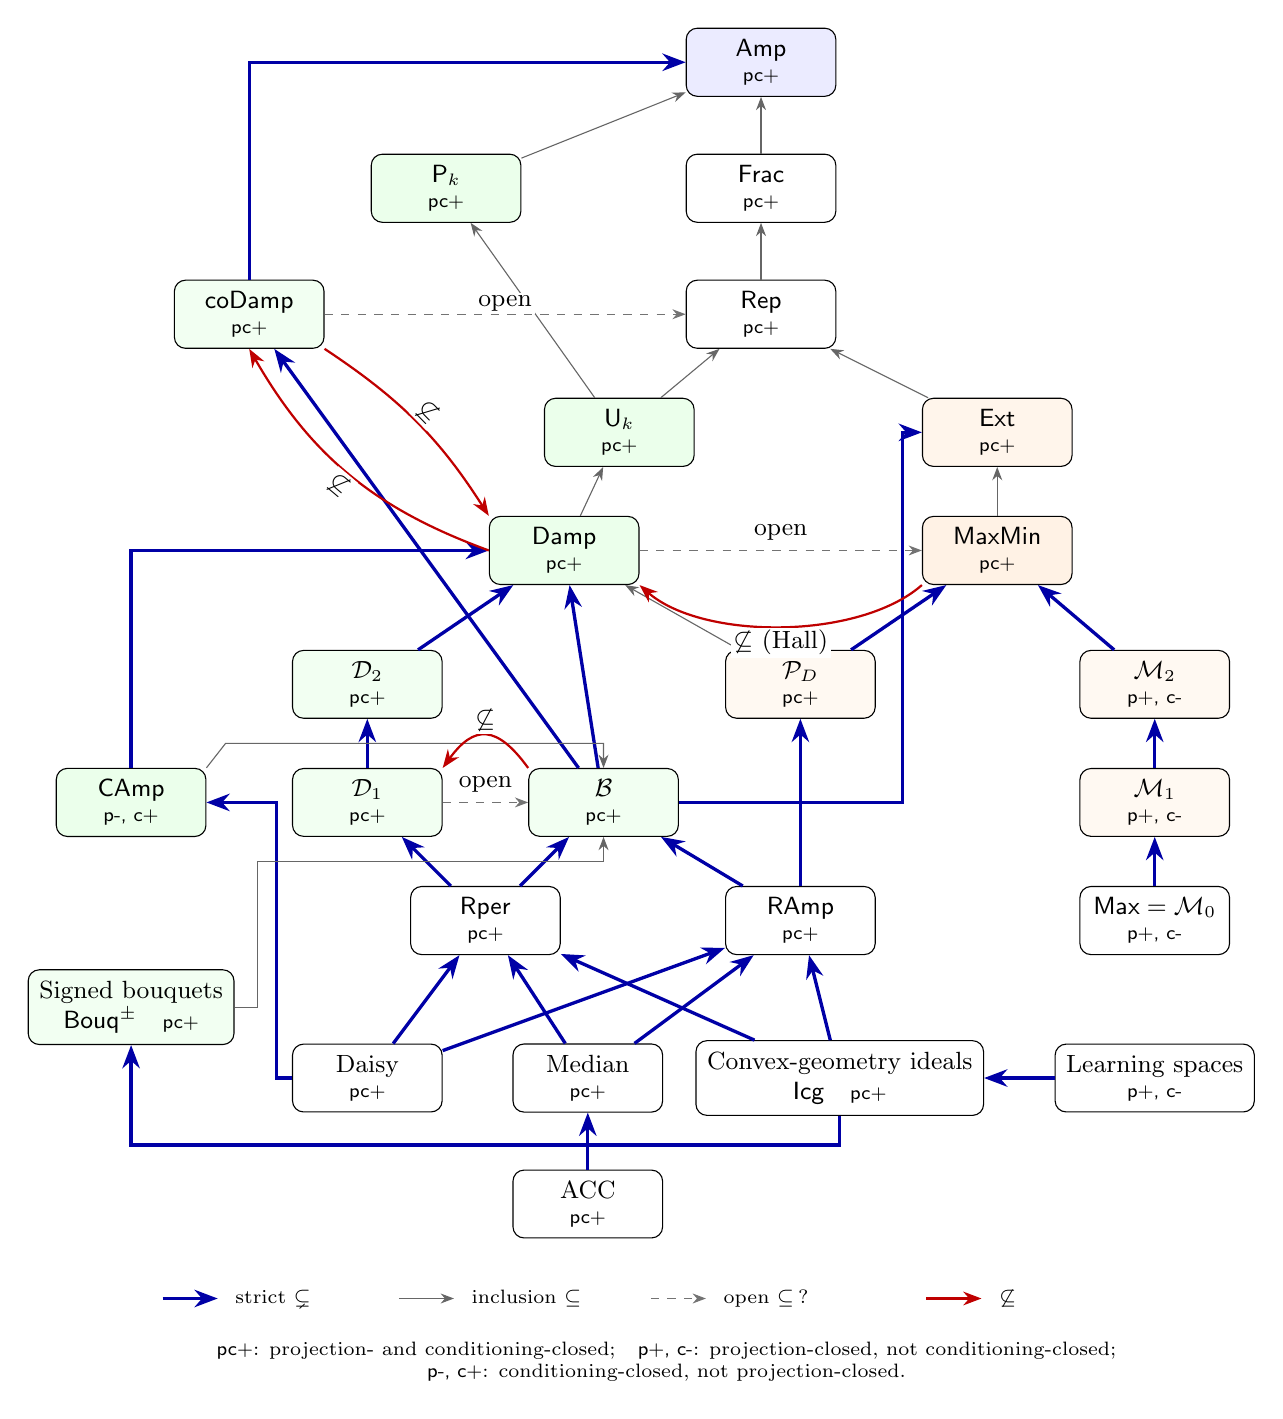
\begin{tikzpicture}[>=Stealth,
 box/.style={draw,rounded corners,align=center,minimum height=.85cm,
             minimum width=1.9cm,font=\small,inner sep=4pt},
 incl/.style={->,draw=black!60,thin},
 strict/.style={->,draw=blue!65!black,line width=1.2pt},
 open/.style={->,draw=black!55,thin,dashed},
 nonincl/.style={->,draw=red!75!black,thick}]
\node[box,fill=blue!8] (amp) at (5,12.7) {$\Amp$\\[-2pt]{\scriptsize\textsf{pc+}}};
\node[box] (frac) at (5,11.1) {$\Frac$\\[-2pt]{\scriptsize\textsf{pc+}}};
\node[box] (part) at (5,9.5) {$\Rep$\\[-2pt]{\scriptsize\textsf{pc+}}};
\node[box,fill=orange!8] (ext) at (8,8) {$\mathsf{Ext}$\\[-2pt]{\scriptsize\textsf{pc+}}};
\node[box,fill=green!5] (codamp) at (-1.5,9.5) {$\mathsf{coDamp}$\\[-2pt]{\scriptsize\textsf{pc+}}};
\node[box,fill=green!8] (damp) at (2.5,6.5) {$\Damp$\\[-2pt]{\scriptsize\textsf{pc+}}};
\node[box,fill=green!8] (uk) at (3.2,8) {$\mathsf U_k$\\[-2pt]{\scriptsize\textsf{pc+}}};
\node[box,fill=green!8] (pk) at (1,11.1) {$\mathsf P_k$\\[-2pt]{\scriptsize\textsf{pc+}}};
\node[box,fill=orange!10] (mm) at (8,6.5) {$\MaxMin$\\[-2pt]{\scriptsize\textsf{pc+}}};
\node[box,fill=orange!5] (pd) at (5.5,4.8) {$\mathcal P_D$\\[-2pt]{\scriptsize\textsf{pc+}}};
\node[box,fill=green!5] (d2) at (0,4.8) {$\mathcal D_2$\\[-2pt]{\scriptsize\textsf{pc+}}};
\node[box,fill=green!5] (d1) at (0,3.3) {$\mathcal D_1$\\[-2pt]{\scriptsize\textsf{pc+}}};
\node[box,fill=green!5] (both) at (3,3.3) {$\mathcal B$\\[-2pt]{\scriptsize\textsf{pc+}}};
\node[box] (rp) at (1.5,1.8) {$\Rper$\\[-2pt]{\scriptsize\textsf{pc+}}};
\node[box] (real) at (5.5,1.8) {$\RAmp$\\[-2pt]{\scriptsize\textsf{pc+}}};
\node[box,fill=orange!5] (m2) at (10,4.8) {$\mathcal M_2$\\[-2pt]{\scriptsize\textsf{p+, c-}}};
\node[box,fill=orange!5] (m1) at (10,3.3) {$\mathcal M_1$\\[-2pt]{\scriptsize\textsf{p+, c-}}};
\node[box] (max) at (10,1.8) {$\Max=\mathcal M_0$\\[-2pt]{\scriptsize\textsf{p+, c-}}};
\node[box] (med) at (2.8,-.2) {Median\\[-2pt]{\scriptsize\textsf{pc+}}};
\node[box] (daisy) at (0,-.2) {Daisy\\[-2pt]{\scriptsize\textsf{pc+}}};
\node[box,fill=green!8] (camp) at (-3,3.3) {$\mathsf{CAmp}$\\[-2pt]{\scriptsize\textsf{p-, c+}}};
\node[box,fill=green!5] (bouq) at (-3,.7) {Signed bouquets\\$\mathsf{Bouq}^{\pm}$\quad{\scriptsize\textsf{pc+}}};
\node[box] (ideals) at (6,-.2) {Convex-geometry ideals\\$\mathsf{Icg}$\quad{\scriptsize\textsf{pc+}}};
\node[box] (learn) at (10,-.2) {Learning spaces\\[-2pt]{\scriptsize\textsf{p+, c-}}};
\node[box] (acc) at (2.8,-1.8) {ACC\\[-2pt]{\scriptsize\textsf{pc+}}};
\foreach \a/\b in {part/frac,frac/amp,mm/ext,ext/part,damp/uk,uk/part,uk/pk,pk/amp,pd/damp}
 \draw[incl] (\a)--(\b);
\foreach \a/\b in {rp/d1,rp/both,d1/d2,d2/damp,both/damp,real/pd,pd/mm,
 max/m1,m1/m2,m2/mm,both/codamp,med/rp,med/real,daisy/rp,
 daisy/real,learn/ideals,ideals/real,real/both,ideals/rp,acc/med}
 \draw[strict] (\a)--(\b);
\draw[strict] (codamp.north) -- (-1.5,12.7) -- (amp.west);
\draw[strict] (both.east) -- (6.8,3.3) -- (6.8,8) -- (ext.west);
\draw[strict] (daisy.west) -- (-1.15,-.2) -- (-1.15,3.3) -- (camp.east);
\draw[strict] (camp.north) -- (-3,6.5) -- (damp.west);
\draw[incl] (camp.north east) -- (-1.8,4.05) -- (3,4.05) -- (both.north);
\draw[strict] (ideals.south) -- (6,-1.05) -- (-3,-1.05) -- (bouq.south);
\draw[incl] (bouq.east) -- (-1.4,.7) -- (-1.4,2.55) -- (3,2.55) -- (both.south);
\draw[open] (codamp)--node[above,font=\small,fill=white,inner sep=1pt] {open} (part);
\draw[open] (damp)--node[above,font=\small] {open} (mm);
\draw[open] (d1)--node[above,font=\small] {open} (both);
\draw[nonincl] (codamp.south east) to[bend left=12]
 node[midway,above,sloped,font=\small,fill=white,inner sep=1pt] {$\not\subseteq$} (damp.north west);
\draw[nonincl] (damp.west) to[bend left=20]
 node[midway,below,sloped,font=\small,fill=white,inner sep=1pt] {$\not\subseteq$} (codamp.south);
\draw[nonincl] (mm.south west) .. controls +(-.8,-.7) and +(.8,-.7) ..
 node[midway,below,font=\small,fill=white,inner sep=1pt] {$\not\subseteq$ (Hall)} (damp.south east);
\draw[nonincl] (both.north west) .. controls +(-.4,.55) and +(.4,.55) ..
 node[midway,above,font=\small,fill=white,inner sep=1pt] {$\not\subseteq$} (d1.north east);
\draw[strict] (-2.6,-3)--(-1.9,-3);
\node[anchor=west,font=\scriptsize] at (-1.8,-3) {strict $\subsetneq$};
\draw[incl] (.4,-3)--(1.1,-3);
\node[anchor=west,font=\scriptsize] at (1.2,-3) {inclusion $\subseteq$};
\draw[open] (3.6,-3)--(4.3,-3);
\node[anchor=west,font=\scriptsize] at (4.4,-3) {open $\subseteq\,?$};
\draw[nonincl] (7.1,-3)--(7.8,-3);
\node[anchor=west,font=\scriptsize] at (7.9,-3) {$\not\subseteq$};
\node[font=\scriptsize,align=center] at (3.8,-3.8)
 {\textsf{pc+}: projection- and conditioning-closed;\quad
  \textsf{p+, c-}: projection-closed, not conditioning-closed;\\
  \textsf{p-, c+}: conditioning-closed, not projection-closed.};
\end{tikzpicture}}
\caption{Selected structural subclasses of ample classes. Solid arrows are
proved inclusions; thick arrows assert strictness, and dashed arrows mark
open inclusions. Red labelled arrows assert noncontainment, not disjointness:
all nodes contain a one-vertex class. An omitted arrow asserts nothing.
Closure badges refer to nonempty minors; for $\mathcal M_k$ the original
ambient coordinates, including constants, are retained.
Here $\mathcal P_D$ means sections of dismantlable maximum parents.
The width families ($k\ge1$) satisfy $\mathsf U_1=\mathsf P_1=\Damp$,
$\bigcup_k\mathsf U_k=\Rep$, $\bigcup_k\mathsf P_k=\Amp$, and
$\mathsf U_k\subseteq\mathsf P_k$.
Allocation and whole-witness refinements appear separately in
\cref{fig:allocation-refinements}. The signed-bouquet arrow into
$\mathcal B$ uses the recent author-proved complementary completion;
\cref{sec:signed-bouquets} records its source and review scope.
The additional $\mathsf{CAmp}\subseteq\mathcal B$ arrow is the
complementary completion theorem in
\cref{prop:atlas-cube-chordal-complement}; it does not settle
$\mathsf{CAmp}\subseteq\MaxMin$.}
\label{fig:classes}
\end{figure}


Median and daisy membership in $\Rper$, and $\Rper\subseteq\Damp$, are
proved in \cite{Cover}. Learning-space membership in $\Rper$ and the
realizability arrows from learning spaces and daisy cubes are proved in
\cite[Section~\textnormal{Downsets and learning spaces}]{MaxParents}.
Learning spaces and, more generally, conditional
antimatroids are corner-peelable \cite[Proposition~4.9]{CCMW}.
Realizable COMs admit corner peelings, and their corners are single vertices
in the ample case \cite[Propositions~5.3 and~5.5]{KM}; hence
$\RAmp\subseteq\Damp$. The maximum-parent construction in \cite{Geometry}
gives $\RAmp\subseteq\MaxMin$, including a direct construction for median
classes. Maximum and corner-peelable ample classes admit representation maps
\cite{CCMW}; their minor descent in \cite{Partition} gives the remaining
arrows. The cornerless maximum example is also from \cite[Theorem~4.5]{CCMW}.
In particular, maximumity must not be placed below corner peelability.

For the lower strict arrows, $\bits^3\setminus\{111\}$ is a realizable
peripheral downset but is not median: the majority of $110,101,011$ is
missing. The four-vertex path $000,100,110,111$ is median, hence peripheral
and realizable, but is not a daisy cube up to signed coordinates. Indeed,
a downset using all three coordinates has a root of degree three, whereas
this path has maximum degree two. The strict learning-space inclusion
follows from the three-leaf-star conditioning below, and strictness from
its minor closure to $\RAmp$ uses the 17-concept example discussed after
\cref{prop:learning-ideal-closure}.

\clearpage
\subsection{Cube-chordal ample classes}
\label{sec:cube-chordal}

Chordality gives another sufficient condition for corner peeling, expressed
in terms of the actual maximal cubes of a class. We collect its definition,
structural descriptions and closure properties here. We introduce the name
\emph{cube-chordal ample} for this class; \emph{daisy cube} is established
terminology \cite{KlavzarMollardDaisy}.
The relative peeling theorem is recalled from the dismantlable-ample
companion, and the tree description from the maximum-ancestry companion.
The product criterion and explicit examples make their consequences precise.
The complementary completion theorem below also puts this class in
$\mathcal B$, where both original ambient shores are corner-peelable.

\begin{definition}[Cube-chordal ample classes]
\label{def:cube-chordal}
For nonempty $H\subseteq\bits^E$, a positioned cube is
\[
 C(p,S)=\{x\in\bits^E:x|_{E\setminus S}=p\},
 \qquad S\subseteq E,\quad p\in\bits^{E\setminus S}.
\]
Its free coordinate set is $S$. Let $\mathcal M(H)$ be the family of
\emph{all} inclusion-maximal positioned cubes contained in $H$.
The maximal-cube intersection graph $\Gamma(H)$ has vertex set
$\mathcal M(H)$; distinct cubes are adjacent exactly when their vertex
sets intersect, including an intersection consisting of one word.
We call $H$ \emph{cube-chordal ample} if $H$ is ample and $\Gamma(H)$
is chordal, meaning that it has no induced cycle of length at least four.
Write $\mathsf{CAmp}$ for this family, and use \emph{cube-chordal} as
shorthand when ampleness is understood.
\end{definition}

The graph uses complete positioned cubes, rather than just their free
coordinate sets or a selected cube cover. Equivalently its vertices are
the extentures of $\bits^E\setminus H$: two such minimal forbidden
patterns are adjacent when their fixed literals are compatible.
Chordality here concerns $\Gamma(H)$, not the one-inclusion graph of $H$;
even a full square has a nonchordal one-inclusion graph.

A \emph{daisy cube rooted at $z$} means that
$\{\operatorname{Diff}(z,x):x\in H\}$ is a downset in $2^E$,
where $\operatorname{Diff}(z,x)=\{i\in E:z_i\ne x_i\}$.
Equivalently, $H$ contains the full cube interval from $z$ to each of
its words: $I(z,x)=\{y:\operatorname{Diff}(z,y)\subseteq
\operatorname{Diff}(z,x)\}\subseteq H$ for every $x\in H$.
Thus the root specifies the Boolean orientation of the established daisy
cube notion recalled above. These classes are ample: if $S$ is shattered,
a word differing from $z$ on all of $S$ supplies the entire rooted
$S$-cube by downward closure.

\begin{proposition}[The complete-graph case]
\label{prop:cube-chordal-daisy}
For a nonempty class $H$, $\Gamma(H)$ is complete if and only if $H$ is
a daisy cube. Consequently
\[
 \mathsf{Daisy}\subsetneq\mathsf{CAmp}\subsetneq\Damp\subseteq\Rep.
\]
There is no bound on VC dimension in $\mathsf{CAmp}$.
\end{proposition}
\begin{proof}
Positioned cubes have the Helly property: pairwise intersection says that
no two fixed literals conflict, so all the fixed literals are jointly
consistent. If $\Gamma(H)$ is complete, all maximal cubes therefore
contain a common word $z$. Each is downward closed towards $z$, and so
is their union $H$. Conversely the maximal cubes of a daisy cube all
contain its root: the top word of any contained cube supplies its whole
rooted lower cube. Thus their intersection graph is complete.

The four-word path $000,100,110,111$ has three maximal edges and
$\Gamma(H)=P_3$. It is ample, since its three directions are distinct,
and is cube-chordal but not a daisy cube. The inclusion into $\Damp$
is proved below, and its strictness by
\cref{ex:cube-chordal-corner}. The last inclusion is the existing
corner-peeling representation theorem. Full cubes give unbounded VC dimension.
\end{proof}

\subsubsection{Daisy pieces, cube attachments and prescribed endpoints}

The following gives an exact construction in the original Boolean
coordinates. It uses the complete extenture family, so no choice of a
redundant forbidden-pattern presentation is implicit.

\begin{proposition}[An incremental construction]
\label{prop:cube-chordal-generator}
Start from any one positioned cube. Given a previously constructed class
$B$, attach $C=C(\delta,S)$, with $Y=E\setminus S$, subject to:
\begin{enumerate}[label=(\roman*)]
\item $C\not\subseteq B$, and $C$ contains no member of $\mathcal M(B)$;
\item the clamp $c(b)=(b|_S,\delta|_Y)$ belongs to $B$ for every $b\in B$;
\item the members of $\mathcal M(B)$ meeting $C$ intersect pairwise.
\end{enumerate}
The outputs are exactly $\mathsf{CAmp}$. Condition~(ii) is equivalent to
\[
 \pi_SB=\pi_S(B\cap C),
\]
and to the following extenture condition: every extenture of $B$ whose
support meets $Y$ has a $Y$-literal opposite to $\delta$.
The interface $F=B\cap C$ is a nonempty proper daisy cube inside $C$,
rooted at a common word of $C$ and all its neighbours.
It is gated in $B$, with gate $c(b)$: for every $b\in B$ and $f\in F$,
\[
 d(b,f)=d(b,c(b))+d(c(b),f).
\]
Here $d$ is Hamming distance, equal to graph distance on the ample pieces.
\end{proposition}
\begin{proof}
First suppose $B$ is ample and (ii) holds. Every cube in $B\cup C$
lies in one piece. Otherwise it contains a new word $v\in C\setminus B$
and frees some $Y$-coordinate; flipping that coordinate at $v$ gives a
word $b$ outside $C$, hence in $B$, with $c(b)=v$, a contradiction.
Also every support shattered by $B\cup C$ that meets $Y$ is already
shattered by $B$. To realize a prescribed trace whose $Y$-part agrees
with $\delta$, first flip one of its prescribed $Y$-bits and realize that
trace in the union. Its witness lies in $B$; clamping gives the desired
trace in $B$. Traces not agreeing with $\delta$ already have witnesses
in $B$. Thus
\[
 \Sh(B\cup C)=\Sh(B)\cup2^S.
\]
The same union describes strongly shattered supports by the cube assertion,
so $B\cup C$ is ample. By (i) its maximal cubes are exactly
$\mathcal M(B)\cup\{C\}$. Condition~(iii) makes the new graph vertex
simplicial, preserving chordality. This proves soundness by induction.

For the converse, use the \href{../maxmin-forbidden/sections/chordal_guard_coefficients.tex}
{simplicial-cube remainder lemma} in the maximum-ancestry companion
(label \nolinkurl{lem:maxmin-simplicial-cube-remainder}).
It states that removing the exclusive words of a simplicial maximal cube
from an ample class leaves an ample $B$ with exactly the other maximal
cubes. Here is the removal argument: cube Helly supplies a common word
$z$ of that cube and its neighbours. Their intersections form a proper
daisy cube $F$ rooted at $z$. Delete the remaining words in decreasing
support inclusion relative to $z$. Each is a corner, because it is maximal
in the remaining downset inside $C$ and belongs to no other old cube.
Every cube of $F$ lies in one neighbouring cube: its top word and $z$
belong to that neighbour's face in $C$. This also proves the exact remaining
maximal-cube list.

For this remainder every cube of $B\cup C$ lies in a piece. Ampleness and
the Sandwich equality $|A|=|\Sh(A)|$ for ample $A$ therefore give
\[
 |\Sh(B)\cap2^S|=|B|+|C|-|B\cup C|=|F|.
\]
Projection preserves ampleness, so $|\pi_SB|=|\Sh(B)\cap2^S|$.
Since $\pi_SF\subseteq\pi_SB$ has $|F|$ words, the projections agree.
This proves (ii); maximality and simpliciality give (i),(iii).
A chordal graph has a simplicial vertex, and deleting it leaves a chordal
graph. Repeat until one maximal cube remains, then reverse the steps.

For the extenture equivalence, an extenture meeting $Y$ with every
$Y$-literal equal to $\delta$ would, by minimality, have its $S$-part
realized in $B$. Clamping that witness would realize the forbidden pattern.
Conversely a clamp avoids every $S$-only extenture because its original
word did, and avoids every other extenture by an opposite $Y$-literal.
Helly and (iii) give the asserted common root and the daisy interface.
It is nonempty by (ii), and proper by (i). Finally $b$ and $c(b)$ differ
only on $Y$, whereas $c(b)$ and $f$ differ only on $S$; this proves the
distance identity and gatedness. Uniqueness follows by putting $f=c(b)$
in the corresponding identity for any proposed gate.
\end{proof}

The interface may be a union of faces rather than a single cube.
For example, attach the three maximal squares of
$\bits^3\setminus\{111\}$ in succession. The last interface is a
three-word path, a daisy cube with two maximal edges. It is gated in the
old host; it need not be gated in the incoming square.

There is also an exact simultaneous tree description. The maximal cliques
of $\Gamma(H)$ have a clique tree: every cube label occurs in a connected
subtree, and intersecting labels occur together in a bag. Each bag union
is a daisy cube rooted at its common word. Adjacent bag unions intersect
in the union of their shared cube labels, a daisy cube rooted at both bag
roots. These assertions, including a converse, are proved in
\href{../maxmin-forbidden/sections/chordal_downset_tree.tex}
{\nolinkurl{thm:maxmin-chordal-downset-tree}}.
The converse requires one additional compatibility condition. Write $d(C)$
for the free coordinate set of a positioned cube $C$. For every
coordinate face $P$ and $S\subseteq d(P)$, the union of occurrence subtrees
of labels $C$ with $C\cap P\ne\varnothing$ and $S\subseteq d(C)$ must
be connected or empty. These are unions of tree vertices \emph{and edges};
adjacent vertices alone do not supply an edge. An arbitrary tree of daisy
cubes need not satisfy this condition and is not an equivalent definition.

\begin{proposition}[Peeling to any contained cube]
\label{prop:cube-chordal-peeling}
If $H\in\mathsf{CAmp}$ and $Q\subseteq H$ is a nonempty positioned
cube, there is a corner order from $H$ to $Q$ in which every remaining
class is cube-chordal ample. Every supplied ordinary representation on $Q$
extends to $H$, with boundary edges directed into $Q$ and no directed
cycle outside $Q$. In particular every vertex can be the final word of
a corner order and the sink of an acyclic ordinary representation of $H$.
\end{proposition}
\begin{proof}
This is the cube-retention theorem
\cite[\nolinkurl{thm:damp-chordal-cube-retention}]{AmpleCampaign}.
We recall the argument to specify the strength of the statement.
A chordal graph has a simplicial vertex outside any proper clique:
a noncomplete chordal graph has two nonadjacent simplicial vertices,
and every vertex of a complete graph is simplicial. Protect the clique
of maximal cubes containing $Q$. If it is proper, choose a simplicial
cube $C$ outside it. Let $z$ be a common word of $C$ and its neighbours,
and $y$ its antipode in $C$. Every neighbouring face contains $z$ and
excludes $y$, so $y$ has unique maximal cube $C$ and is a corner outside $Q$.
If all maximal cubes contain $Q$ and $H\ne Q$, choose any such $C$,
take $z\in Q$, and again its antipode $y\notin Q$ is a corner.

Deleting $y$ replaces $C$ by its facets opposite $y$, discarding facets
contained in unchanged cubes. The retained facets form a clique with
exactly the old clique neighbourhood of $C$, since they all contain $z$.
Each is simplicial, so chordality is preserved. Corner deletion preserves
ampleness. Induction reaches $Q$.
Reverse the order, adding each removed corner as a source. This extends
an ordinary representation by the corner-extension theorem, preserves the
map on $Q$, and makes its boundary inward. A directed cycle cannot use
an added vertex: the last added vertex on that cycle would have only
outgoing edges to earlier vertices. For a prescribed single-vertex target,
its trivial map therefore extends acyclically with that vertex as sink.
\end{proof}

\begin{samepage}
\subsubsection{Corner peelings on both ambient shores}

\begin{proposition}[Complementary completion of cube-chordal classes]
\label{prop:atlas-cube-chordal-complement}
If $H\subseteq\bits^E$ is nonempty and cube-chordal ample, then both $H$
and its full original ambient complement have corner peelings. Consequently
\[
 \mathsf{CAmp}\subseteq\mathcal B\subsetneq\mathsf{Ext}.
\]
There is no bound on VC dimension. Original constant coordinates are retained;
an empty complement has the empty map and peeling order.
\end{proposition}
\end{samepage}
\begin{proof}
Apply the tree completion theorem
\cite[\texttt{prop:leaf-root-alignment}, \texttt{thm:camp-ext}]{CubeComplementCompletion}.
Its input is the positioned tree of daisy pieces recalled above: every
connected subunion is ample, every cube is carried by a piece, word
occurrences are connected, and each adjacent overlap is rooted at both
piece roots. The theorem supplies a finite increasing sequence
$H=H_0\subset\cdots\subset H_m=L$, where $L$ is one daisy cube.
Each step attaches a cube $Q(z,S)$ whose clamp preserves $H_j$ and whose
intersection with $H_j$ is a nonempty daisy rooted at $z$.
The construction preserves the tree properties; it does not assume that
intermediate maximal-cube graphs remain chordal.

For completeness, such a step gives an explicit complementary peeling.
The added words $A=Q(z,S)\setminus H_j$ form an up-set towards the corner
opposite $z$. Remove them from $H_j^c$ in increasing distance from $z$.
At the removal of $a$, put $D=\operatorname{Diff}(a,z)\subseteq S$.
Rootward neighbors are old words or were removed earlier. The entire
cube with directions $E\setminus D$ remains: its traces in $Q(z,S)$
are later words of $A$, and all parallel outside words are absent from
$H_j$ by clamp invariance. Thus $a$ is an actual corner with that support.
The remaining class is $H_{j+1}^c$. After all steps, peel the up-set $L^c$
in increasing distance from its daisy root. The primal peeling is
\cref{prop:cube-chordal-peeling}. This proves membership in $\mathcal B$;
$\mathcal B\subsetneq\mathsf{Ext}$ was established in
\cref{prop:maxmin-neighbors}.
\end{proof}

Neither complementation nor projection must preserve cube chordality.
The conclusion above concerns the two shores' corner peelings, not their
maximal-cube graphs. It also does not supply maximum parents:
$\mathsf{CAmp}\subseteq\MaxMin$ remains open.
Conversely, if an ample $H$ is not corner-peelable, then neither $H$ nor
$H^c$ is cube-chordal. Thus both maximal-cube intersection graphs contain
an induced cycle of length at least four; this is a necessary condition,
not a characterization of nondismantlability.

\subsubsection{Closure properties and the exact product criterion}

In the table, empty results may be adjoined formally. A full reduction on
$I$ keeps exactly those words whose entire $I$-fiber is present:
\[
 H^I=\{x\in\bits^{E\setminus I}:\{x\}\times\bits^I\subseteq H\}.
\]
A rooted vertex wedge identifies specified vertices of two classes on
disjoint coordinate blocks, keeping all coordinates of the other block
fixed at that vertex in each piece.

\begin{center}
\begin{tabular}{@{}p{.72\linewidth}l@{}}
\toprule
Operation & Preserves $\mathsf{CAmp}$?\\
\midrule
Signed coordinate isometries; adding or suppressing constants & Yes\\
Coordinate faces; geodesically convex subclasses & Yes\\
Full coordinate reductions $H^I$ & Yes\\
Rooted vertex wedges on disjoint blocks & Yes\\
Product with any daisy cube & Yes\\
Arbitrary Cartesian products & No\\
Coordinate projections; arbitrary pc-minors & No\\
Complementation in the specified ambient cube & No\\
Arbitrary corner deletion or corner addition & No\\
Gluing along a common cube, even a convex coordinate face & No\\
Arbitrary ample subclasses & No\\
\bottomrule
\end{tabular}
\end{center}

\begin{proposition}[Faces, reductions and vertex wedges]
\label{prop:cube-chordal-closures}
The affirmative closure assertions in the table hold.
\end{proposition}
\begin{proof}
Signed isometries and constants preserve the maximal-cube graph.
For a coordinate face $P$, its maximal cubes in $H\cap P$ are the maximal
nonempty traces $C\cap P$ of old maximal cubes. Choose one old cube for
each such trace. Two retained traces intersect if and only if their old
representatives intersect: the reverse implication uses cube Helly on
the two representatives and $P$. Thus $\Gamma(H\cap P)$ is isomorphic
to an induced subgraph of $\Gamma(H)$ and is chordal. Faces preserve
ampleness. Convex subclasses of a partial cube are intersections of its
coordinate halfspaces, as recalled in the operations section, so are faces.

For reduction, the maximal cubes of $H^I$ correspond exactly to the old
maximal cubes freeing every coordinate of $I$, with $I$ removed.
Indeed lift a reduction cube to its product with $\bits^I$ and extend it
to a maximal cube of $H$; maximality on either side gives the converse.
Intersections are preserved, so the graph is again induced. Full reductions
preserve ampleness by iterating the usual ample two-sided reduction.

Singleton wedge factors are neutral. Otherwise all maximal cubes come
from one factor. Cubes from different factors meet exactly when both
contain the identified root. The root-containing cubes of each factor
form a clique. Glue the two chordal graphs to the complete graph on
their combined root-containing cubes, along these two cliques.
Clique gluing preserves chordality: an induced cycle visiting both sides
of a clique separator would have a chord. Finally a shattered support
cannot use a nonconstant coordinate from each private block, since the
pattern opposite both roots is absent. Supports wholly in one block are
shattered exactly when that factor shatters them, and are strongly
shattered there. Thus the wedge is ample. Product closure with daisy cubes
is the next proposition.
\end{proof}

\begin{proposition}[Exact product criterion]
\label{prop:cube-chordal-product}
For any nonempty ample $H,K$ on disjoint coordinate sets,
\[
 H\times K\in\mathsf{CAmp}
 \quad\Longleftrightarrow\quad
 H,K\in\mathsf{CAmp}\ \text{and at least one factor is a daisy cube}.
\]
\end{proposition}
\begin{proof}
Products of ample classes are ample: a support is shattered, or strongly
shattered, exactly when its two factor supports are. The maximal cubes
of a product are precisely the products of maximal cubes. Consequently
$\Gamma(H\times K)=\Gamma(H)\boxtimes\Gamma(K)$, the strong graph
product: two distinct pairs are adjacent when, in each coordinate, their
entries are equal or adjacent. Fixing either graph entry gives the other
graph as an induced subgraph, so both graphs must be chordal.

These graphs are connected. Indeed an ample class is connected, and
its vertex paths give overlap chains of maximal cubes. Any connected
noncomplete graph contains an induced path on three vertices: use the
first three vertices of a shortest path between nonadjacent vertices.
If both factor graphs are noncomplete, choose such paths indexed $0,1,2$.
The four pairs
\[
 (0,1),\ (1,0),\ (2,1),\ (1,2)
\]
form an induced four-cycle in their strong product. Thus at least one
graph must be complete. Conversely, a strong product with a complete
graph replaces each vertex of the other graph by a clique, giving all
vertices in that clique the same outside neighbours. Replacing each
vertex in a perfect elimination order by its whole clique gives a
perfect elimination order of the product. Chordality is preserved.
Apply \cref{prop:cube-chordal-daisy} to identify the complete factor.
\end{proof}

For instance the four-word path in
\cref{prop:cube-chordal-daisy} is cube-chordal, whereas its product
with itself is not. This product is median, hence in $\Rper$.
Thus even median or recursively peripheral membership does not imply
cube-chordality.

\subsubsection{Explicit failures of closure}

For compact examples, encode $x\in\bits^{\{0,\ldots,n-1\}}$ by
$\sum_i2^ix_i$. Write $Q(a,s)$ for the cube whose free coordinates
are the one-bits of $s$ and whose fixed one-bits are those of $a$;
the two masks have disjoint one-bits. Thus its words are $a\mathbin{\mathrm{or}}t$
for the submasks $t$ of $s$. All lists below are complete maximal-cube lists.

\begin{example}[Corner changes and common-cube gluing]
\label{ex:cube-chordal-corner}
On four coordinates let
\[
 A=\{0,1,2,3,6,7,8,9,10\},\qquad D=A\cup\{5\},\qquad
 U=D\cup\{4\}=\{0,1,\ldots,10\}.
\]
Their maximal cubes, listed as $(a,s)$, are
\begin{align*}
 \mathcal M(A)&:\ (0,3),(2,5),(0,9),(0,10),\\
 \mathcal M(D)&:\ (0,3),(2,5),(1,6),(0,9),(0,10),\\
 \mathcal M(U)&:\ (0,7),(0,9),(0,10).
\end{align*}
These lists follow by extending each edge and face in the displayed
word sets. In $D$, the four cubes
$(2,5),(1,6),(0,9),(0,10)$ form an induced four-cycle in that order;
$(0,3)$ meets all four. Thus $\Gamma(D)$ is the wheel on five vertices,
whereas $\Gamma(A)$ is a diamond and $\Gamma(U)$ is complete.

The class $U$ is a daisy cube rooted at zero. The word $4$ is its corner
with incident free mask $7$, so $D$ is ample and dismantlable.
The word $5$ is a corner of $D$ with incident free mask $6$, leaving $A$.
Hence $U\mapsto D$ disproves closure under corner deletion, and
$A\mapsto D$ disproves closure under corner addition. The inclusion
$D\subseteq\bits^4$ also disproves closure under ample subclasses.
Since $D\in\Damp\setminus\mathsf{CAmp}$, the inclusion into $\Damp$
is strict.

Moreover $D$ is the union of the two daisy cubes
\[
 Z=\{0,1,2,3,5,6,7\},\qquad W=\{0,1,2,3,8,9,10\},
\]
rooted at $3$ and $0$, respectively. Their intersection is the full
square $\{0,1,2,3\}$, a coordinate face and therefore convex in each.
This disproves common-cube gluing closure even for daisy input pieces.
\end{example}

\begin{example}[Projection and complementation]
\label{ex:cube-chordal-projection}
On five coordinates put
\[
 V=\{0,1,2,3,6,7,8,9,16,17,18,19,21,23,24,26\}.
\]
Its maximal cubes are
\[
 (0,19),(2,5),(17,6),(0,9),(16,10),(3,20),(0,24).
\]
Their graph is the cone over two disjoint three-vertex paths and is
chordal. Ampleness can be verified directly. At $x_2=x_3=0$ there is a
full cube on coordinates $\{0,1,4\}$. At $x_2=1$ there is a four-word
path on these coordinates using each direction once, and the same holds
at $x_3=1$. No word has $x_2=x_3=1$. Consequently the shattered supports
are the eight subsets of $\{0,1,4\}$, together with
$\{\{j\}\}\cup\{\{j,i\}:i\in\{0,1,4\}\}$ for each $j=2,3$.
Each is strongly shattered by the central cube, a vertical edge or a
path-edge square. Hence $V$ is ample. Projecting away coordinate $4$
gives exactly $D$ of \cref{ex:cube-chordal-corner}, proving failure
of projection closure and therefore pc-minor closure.

For complementation take the four-coordinate path
$P=\{0,1,3,7,8\}$. Its four edge directions are distinct, so it is
maximum of VC dimension one, with a path as maximal-cube graph.
Its complement is ample by ample complement duality and has maximal cubes
\[
 (12,3),(10,5),(9,6),(4,9),(4,10),(2,12).
\]
The cubes $(10,5),(9,6),(4,9),(4,10)$ form an induced four-cycle in
that order. This proves failure of complement closure.
\end{example}

\subsubsection{Comparison with ACC and maximum ancestry}

Recall that an ACC class has a join tree on its individual maximal
cubes, as defined before \cref{fig:classes}; see also the
\href{../../../YangDim/yang_complex_dictionary.tex}{Yang-complex dictionary}.
A clique tree of $\Gamma(H)$ instead has \emph{bags} of cubes as nodes.
These two requirements are incomparable.

\begin{example}[Neither ACC nor medianity characterizes cube-chordality]
\label{ex:cube-chordal-acc}
The daisy cube $\bits^3\setminus\{111\}$ is cube-chordal, but its three
maximal squares admit no join tree. Each pair has a word belonging to
just those two squares, forcing each of the three possible tree edges.
Even medianity does not repair the implication: the $3$-by-$3$ grid is
a median daisy cube with four maximal squares sharing its middle vertex,
so $\Gamma=K_4$. Each of the four neighbours of that vertex belongs
to just one cyclically consecutive pair of squares. Those four pairs
would all have to be edges of a join tree, which is impossible.

Conversely take a central square and attach a square along each of its
four boundary edges, using a separate private coordinate for each leaf.
The central square and its four leaves have a join tree given by the star.
The class is isometric: within a leaf use square paths; between different
leaves, turn off their distinct private coordinates and take a shortest
path in the central square. It is also ample: its shattered supports are
the empty set, six singletons and the five pairs supporting its squares,
all strongly shattered. Thus it is ACC. Its four leaf squares meet in
an induced four-cycle, so its maximal-cube graph is nonchordal.
\end{example}

\begin{proposition}[Minor closure of ACC]
\label{prop:atlas-acc-closure}
The ACC classes are closed under nonempty projections and conditionings.
Their inclusion into Median is strict.
\end{proposition}
\begin{proof}
Use the characterizations in
\cite[Theorem~\textnormal{ACC characterizations}]{Survey}.
For a median class the split-incompatibility graph has one vertex for
each nonconstant coordinate, joining a pair exactly when it is shattered.
Projection retains its induced graph on the remaining active coordinates.
Chordality and medianity are preserved, proving projection closure.

For conditioning, let $G^\Delta$ join two concepts whenever a contained
cube contains both. If $F$ is a coordinate face, intersecting an old cube
with $F$ shows that $(G\cap F)^\Delta$ is the induced subgraph
$G^\Delta[V(G)\cap F]$. An ACC class has chordal $G^\Delta$;
its induced subgraph is chordal as well. The nonempty coordinate face
is median, so the same characterization proves it ACC.
The median $3$-by-$3$ grid in \cref{ex:cube-chordal-acc} is not ACC,
proving strictness.
\end{proof}

We have proved
$\mathsf{Daisy}\subsetneq\mathsf{CAmp}\subsetneq\Damp$.
The product of the four-word path with itself proves
$\Rper\not\subseteq\mathsf{CAmp}$.
For the other direction the peripheral companion's
\href{../cover-recursive/research/rper_chordal_sun_obstructions.tex}
{chordal sun family} has chordal maximal-cube graph and is forbidden for
$\Rper$. Hence $\mathsf{CAmp}\not\subseteq\Rper$ as well.
Those suns do have maximum parents, as shown in
\href{../maxmin-forbidden/research/chordal_sun_parents.tex}
{\nolinkurl{thm:maxmin-chordal-sun-parents}}.
The unrestricted inclusion $\mathsf{CAmp}\subseteq\MaxMin$ remains open;
neither a clique tree nor the local generator supplies compatible maximum
parents for arbitrary daisy interfaces. The class is not pc-minor closed,
so a forbidden-pc-minor basis cannot characterize membership in
$\mathsf{CAmp}$ itself.


\subsection{The decomposition hierarchy and complementary peeling}\label{sec:intermediate}

For $J\subseteq X$ and $p\in\bits^J$, let $A[p]$ denote the conditioning
of $A\subseteq\bits^X$ at $p$, viewed on $X\setminus J$.
Define $\mathcal D_k$, for $k\ge0$, recursively from singletons by
\begin{equation}\label{eq:decomposition-attachment}
 \begin{gathered}
 C=A\cup(S\times\{p\}),\qquad 1\le |J|\le k+1,\qquad A[p]=\varnothing,\\
 A\in\mathcal D_k,\qquad
 \varnothing\ne S\in\mathcal D_k\text{ on }X\setminus J,\qquad
 S\subseteq A[q]\quad(q\in\bits^J\setminus\{p\}).
 \end{gathered}
\end{equation}
All other block patterns already occur over every word of $S$.
For $|J|=1$ this is the peripheral construction. The next level
$\mathcal D_1$ also permits $|J|=2$, completing squares over a whole
class of words, rather than necessarily adding one vertex. The level
$\mathcal D_2$ permits $|J|\le3$, so it can complete one missing
pattern of a three-dimensional cube over a whole class of words.
All levels satisfy
\[
 \Rper=\mathcal D_0\subseteq\mathcal D_1\subseteq\mathcal D_2
 \subseteq\cdots,\qquad \bigcup_{k\ge0}\mathcal D_k=\Damp.
\]
The primary comparison considered here is $\mathcal D_1\subseteq\mathcal B$.
The exact polygon theorem below proves $\mathcal D_1\subsetneq\mathcal D_2$
and, more generally, strictness at every consecutive level.

The Yang complex $\Delta_C$ has facets $\{(i,c_i):i\in X\}$ for $c\in C$.
Equivalently, $C\in\mathcal D_k$ when $\Delta_C$ is pure
$k$-decomposable: it is a simplex, or a nonempty face of size at most
$k+1$ has a deletion of the same pure dimension, with both deletion and
link recursively satisfying this condition. Deletion removes faces
containing the selected face; its link consists of disjoint faces whose
union with it is a face. The exact equivalence with
\eqref{eq:decomposition-attachment} is proved in \cite{RecursiveClasses}.
In particular,
\[
 \mathcal D_0=\Rper,\qquad \bigcup_{k\ge0}\mathcal D_k=\Damp.
\]
The second identity is the Yang shellability--corner-peeling correspondence.

The attachment also has an exact shattering formula, valid for any ample
$A,S$ satisfying the section conditions in \eqref{eq:decomposition-attachment}:
\begin{equation}\label{eq:attachment-shattering}
 \Sh(C)=\Sh(A)\ \dot\cup\ \{J\cup T:T\in\Sh(S)\}.
\end{equation}
A support not containing $J$ sees no new trace: flip a new word in an
omitted block coordinate to reach an old word. A support $J\cup T$ is
shattered precisely when its $p$-section, supplied by $S$, shatters $T$;
all other block sections contain $S$. None was shattered in $A$, whose
$p$-section is empty. Thus $|\Sh(C)|=|A|+|S|=|C|$, proving ampleness.

For the second family, write $C^c=\bits^X\setminus C$ and set
\begin{equation}\label{eq:both-dismantlable}
 \mathcal B=\{\varnothing\ne C\subseteq\bits^X:
 C\in\Damp,\quad C^c\in\Damp\cup\{\varnothing\}\}.
\end{equation}
The complement uses the displayed ambient cube. Membership is nevertheless
unchanged by adding or suppressing constants: the complement of
$C\times\{0\}$ is $(C^c\times\{0\})\cup(\bits^X\times\{1\})$.
Build the upper cube first, then append lower words in an ample-prefix
order of $C^c$. Every prefix is an ample peripheral expansion. Conversely,
condition the new coordinate to zero. This proves constant stability and
justifies the atlas's signed-coordinate graph convention for $\mathcal B$.

\begin{proposition}[Established intermediate inclusions]
\label{prop:intermediate-inclusions}
The following inclusions are strict:
\[
 \Rper\subsetneq\mathcal D_1\subsetneq\Damp\subsetneq\Amp,
 \qquad \Rper\subsetneq\mathcal B\subsetneq\Damp.
\]
Every ample class of VC dimension at most two belongs to $\mathcal D_1$.
Each $\mathcal D_k$ and $\mathcal B$ is closed under nonempty pc-minors,
two-sided reductions, and Cartesian products. The family $\mathcal B$ is
also complement closed when its empty boundary case is adjoined.
\end{proposition}
\begin{proof}
The recursive inclusions and the VC-two assertion are
\cite{RecursiveClasses}; the latter uses corner peelability in VC
 dimension two \cite[Proposition~4.11]{CCMW}. More generally, a
corner-peelable VC-$d$ class belongs to $\mathcal D_{d-1}$ for $d\ge1$:
the corner's maximal cube supplies a shedding face on at most $d$ literals.
The minor, reduction and product laws follow by induction through
\eqref{eq:decomposition-attachment}, including operations inside the
attached block \cite{RecursiveClosure}.

The pentagonal maximum VC-two class $P_5$ lies in
$\mathcal D_1\cap\mathcal B$ but not in $\Rper$. On a cyclic set of
five coordinates, its positive supports are the empty set, all singletons,
the pentagon's edges, and the complements of those edges.
The source \cite{RecursiveClasses} gives an explicit one-decomposition;
its cube complement is equivalent to the same class by reorientation
and permutation. Its nonperipherality is also recorded in \cite{Cover}.
Peripheral classes are complement closed, so $\Rper\subsetneq\mathcal B$.

Let $H$ be Hall's cornerless maximum VC-three class on twelve coordinates.
Its complement $H^c$ is dismantlable and maximum of VC dimension eight,
whereas $H$ is not dismantlable \cite{RecursiveClasses,OrientationClasses}.
These facts give $\mathcal B\subsetneq\Damp\subsetneq\Amp$.
Moreover, $H^c\notin\mathcal D_1$: a first decomposition face on a
block $J$ would require some section $H[p]$ to equal the projection of
$H$ onto the other coordinates. The exhaustive one- and two-coordinate
section check in \cite{RecursiveClosure} rules this out: the largest
section sizes are 198 and 144, smaller than the respective projection
sizes 232 and 176. This proves $\mathcal D_1\subsetneq\Damp$.

For the closure claims about $\mathcal B$, first note that $\Damp$ is
reduction-closed by its union description above. Write
$\partial_i C=C_i^0\cap C_i^1$ and $\pi_i C=C_i^0\cup C_i^1$.
Complements on the remaining coordinates satisfy
\[
 (C_i^b)^c=(C^c)_i^b,\qquad
 (\pi_i C)^c=\partial_i(C^c),\qquad
 (\partial_i C)^c=\pi_i(C^c).
\]
These identities prove minor and reduction closure, with empty
complementary outputs allowed. Product closure follows from the
orientation characterization below.
\end{proof}

That characterization gives a second description of $\mathcal B$.
An \emph{acyclic unique-sink orientation} of a cube has no directed cycle
and has exactly one sink on every nonempty coordinate face. A set is
\emph{forward invariant} if no directed edge leaves it. For a nonempty
proper class $C$, the complementary-orientation theorem \cite{OrientationClasses} gives
\begin{equation}\label{eq:both-orientation}
 C\in\mathcal B\quad\Longleftrightarrow\quad
 C\text{ is forward invariant in some acyclic unique-sink cube orientation}.
\end{equation}
One direction glues acyclic representation orientations of the two
complementary dismantlable classes, with every crossing edge pointing into
$C$. In the other, restriction to $C$ and reversal on $C^c$ give acyclic
representation orientations, hence corner peelings. This is the exact
source theorem; acyclicity is essential for this dismantlability conclusion.
For product closure, orient each product edge by its factor orientation.
Every face has the pair of its factor sinks, and a sum of topological
orders strictly increases along edges. The product orientation is therefore
acyclic with unique sinks. The product of two forward-invariant sets is
forward invariant. Full factors use any uniform cube orientation, covering
the boundary cases in the product assertion.

Realizable ample classes supply an established subclass of the intersection:
\[
 \RAmp\subseteq\mathcal B\cap\MaxMin.
\]
For proper classes, Lawrence's complement-closure theorem for convex realizability,
proved in the current sign conventions in
\cite[Proposition~\textnormal{Complement closure of convex realizability}]{MaxParents},
puts both complementary classes in $\RAmp\subseteq\Damp$. Full cubes
belong to $\mathcal B$ by the empty-complement convention.
This does not prove $\mathcal B\subseteq\MaxMin$.

\begin{example}[A nonrealizable peripheral class]\label{ex:e26-strictness}
The same 26-word class $E_{26}$ proves both
\[
 \RAmp\subsetneq\mathcal B,
 \qquad \mathsf{Icg}\subsetneq\Rper.
\]
Here is its definition and the obstruction to realization; full separation
details and the independently verified maximum parent are recorded in
\cite{Structural984}. Let $Y=\{a_1,a_2,b_1,b_2\}$ and use two further
coordinates $i,j$, with signs $-$ and $+$ denoting bits zero and one.
For $S\subseteq Y$, define its allowed control labels $K_S$ by
\[
\begin{array}{c|c}
 S & K_S\\ \hline
 \varnothing & \{--,-+,+-,++\}\\
 \varnothing\ne S\subseteq\{a_1,a_2\} & \{--,-+,+-\}\\
 \varnothing\ne S\subseteq\{b_1,b_2\} & \{-+,+-,++\}\\
 \{a_1,b_1\},\ \{a_2,b_2\} & \{-+\}\\
 \{a_2,b_1\},\ \{a_1,b_2\} & \{+-\}\\
 \text{all other }S & \varnothing
\end{array}
\qquad
 E_{26}=\{(\mathbf1_S,z):z\in K_S\}.
\]
The table decreases under inclusion of $S$, so the four coordinates in
$Y$ have nested shores. Split successively in these coordinates, suppressing
constant coordinates. Every remaining nonempty class is a square, a
three-vertex path, or a singleton. These belong to $\Rper$, and the
two-child peripheral recursion therefore proves $E_{26}\in\Rper$.
Complement closure of $\Rper$ gives $E_{26}\in\mathcal B$.

Suppose affine functions $x_1,x_2,y_1,y_2,t,u$ realize this class on an
open convex domain. Its minimal missing sign patterns include
$x_r,t,u>0$ and $y_s>0,t,u<0$, for $r,s\in\{1,2\}$.
Separating each missing orthant cylinder from the convex image gives
inequalities valid throughout the domain,
\[
 h_rx_r+p_rt+q_ru\le0,
 \qquad k_sy_s-r_st-s_su\le0,
\]
with every displayed coefficient strictly positive: separation gives
nonnegative coefficients, and minimality excludes any zero coefficient.
Set $\alpha_r=q_r/p_r$ and $\beta_s=s_s/r_s$.
An allowed word with $x_r,y_s>0$ and control label $-+$ forces
$\alpha_r<|t|/u<\beta_s$; a word with control label $+-$ forces
$\beta_s<t/|u|<\alpha_r$.
The four mixed-pair rows consequently give
\[
 \alpha_1<\beta_1<\alpha_2<\beta_2<\alpha_1,
\]
a contradiction in every ambient realization dimension. Thus
$E_{26}\in\Rper\setminus\RAmp$. Since
$\mathsf{Icg}\subseteq\Rper\cap\RAmp$ by
\cref{prop:learning-ideal-closure} and the learning-space minor-closure
results, this proves both asserted strict inclusions.
\end{example}

\subsection{Exact decomposition levels of polygon complements}
\label{sec:polygon-decomposition}

Complements of regular tangent-line arrangements separate every consecutive
pair of decomposition levels. For a nonempty dismantlable class, define
its \emph{decomposition level} by
\[
 \kappa(C)=\min\{k\ge0:C\in\mathcal D_k\}.
\]
The minimum exists because $\bigcup_k\mathcal D_k=\Damp$.
We first record the necessary first-face condition and a peripheral family
used to construct decompositions attaining the lower bound.

For $C\subseteq\bits^X$, write $H=\bits^X\setminus C$.
If a nonempty face $(J,p)$ begins a decomposition of $C$ by
\eqref{eq:decomposition-attachment}, then
\begin{equation}\label{eq:dominant-complement-shore}
 H[q]\subseteq H[p]\quad(q\in\bits^J),\qquad
 H[p]=\pi_{X\setminus J}H.
\end{equation}
Indeed, $C[p]$ is contained in every other $J$-shore. Complementing
these inclusions and taking their union proves the assertions.

\begin{lemma}[Intervals with two endpoint cubes]
\label{lem:interval-endpoint-cubes}
On the linearly ordered set $[L]=\{1,\ldots,L\}$, let $\mathcal I_L$
consist of the empty set and all linear intervals. For $0\le a,b\le L$,
the family
\[
 K_{L,a,b}=\mathcal I_L\cup2^{[a]}
              \cup2^{\{L-b+1,\ldots,L\}}
\]
is recursively peripheral. Its complement is recursively peripheral
whenever nonempty. A cube on the empty support means the singleton
empty set.
\end{lemma}
\begin{proof}
First let $P_{t,a}$ consist of all prefixes of $[t]$, including the
empty prefix, together with $2^{[a]}$, where $0\le a\le t$.
If $t=a$, this is a cube. If $t>a$, its last-coordinate sections are
$P_{t-1,a}$ and $\{[t-1]\}$; the latter is contained in the former.
Induction and the peripheral recursion prove $P_{t,a}\in\Rper$.

Now induct on $L$. The case $L=0$ is a singleton. If $a=L$ or
$b=L$, the family $K_{L,a,b}$ is a cube. Otherwise its
first-coordinate sections, after renumbering the remaining path, are
\[
 K_{L,a,b}[0]=K_{L-1,\max(a-1,0),b},\qquad
 K_{L,a,b}[1]=P_{L-1,\max(a-1,0)}.
\]
Every prefix is an interval, so the second section is contained in the
first. Both are recursively peripheral by induction, proving the claim.
Complement closure of $\Rper$ gives the final assertion.
\end{proof}

\begin{proposition}[Exact levels of tangent-polygon complements]
\label{prop:polygon-decomposition}
For $m\ge2$, put $n=2m+1$ and
$v_j=(\cos(2\pi j/n),\sin(2\pi j/n))$ for $0\le j<n$.
Let $H_n\subseteq\bits^n$ consist of the strict sign words of
$v_j\cdot x-1$ on $\mathbb R^2$, with positive sign encoded by one,
and let $C_n=\bits^n\setminus H_n$. Then $H_n$ and $C_n$ are
convexly realizable maximum classes of ranks two and $n-3$, respectively,
both belong to $\mathcal B$, and
\begin{equation}\label{eq:exact-polygon-level}
 \kappa(H_{2m+1})=1,\qquad \kappa(C_{2m+1})=m-1.
\end{equation}
Consequently, for every $k\ge0$,
\[
 \mathcal D_k\subsetneq\mathcal D_{k+1},
\]
with realizable maximum witness $C_{2k+5}$.
Moreover, $\mathcal B$ and $\RAmp$ are contained in no fixed
$\mathcal D_k$, and every $\mathcal D_k$ with $k\ge1$ fails
closure under cube complementation.
\end{proposition}
\begin{proof}
The proof first determines the smallest possible attachment block, then
constructs a decomposition with exactly that block-size bound.

The lines $v_j\cdot x=1$ are tangents to the unit circle. Since $n$
is odd, none are parallel; no three concur because a point has at most
two tangents to a circle. The arrangement therefore has
$1+n(n+1)/2$ regions with distinct sign words. Every pair of lines
realizes all four patterns, whereas every triple has seven regions.
Thus $H_n$ is maximum of rank two. Maximum complementation gives rank
$n-3$ for $C_n$, and Lawrence's complement theorem gives its convex
realizability. Realizable corner peeling puts both classes in $\Damp$,
so both lie in $\mathcal B$.
Identify a word with its positive support in the cyclically ordered set
$X=\{0,\ldots,n-1\}$. Then $H_n$ consists of the empty set and all
cyclic intervals of lengths one through $m+1$. Indeed, a point outside
the unit circle selects the normals in an open arc of width less than
$\pi$; varying its direction and distance realizes exactly these
intervals. Points inside give the empty set.

We claim that among nonempty blocks $J$ with $|J|\le m$,
\eqref{eq:dominant-complement-shore} holds precisely when $J$ is a
consecutive $m$-block and $p=0_J$. Put $W=X\setminus J$.
Suppose first that $p_i=1$ for some $i\in J$. Let $a,b\in W$ be
the nearest retained coordinates before and after $i$. Since
$|W|\ge m+1\ge3$, choose $w\in W\setminus\{a,b\}$.
The singleton trace $\{w\}$ occurs in the projection of $H_n$.
But either cyclic path from $i$ to $w$ meets another retained coordinate,
namely $a$ or $b$. No interval containing $i$ can have trace $\{w\}$
on $W$. Thus the required equality fails, and a possible pattern must
be $0_J$.

Take a maximal run of deleted coordinates of length $g$, with retained
endpoints $a,b$. If $g\le m-1$, the interval comprising the run and
its endpoints has length $g+2\le m+1$, so $\{a,b\}$ occurs in the
projection. To realize this trace at $0_J$, the positive set would
have to be exactly $\{a,b\}$. This is not an interval: one path
between the endpoints contains the deleted run, and the other contains
another retained coordinate. Hence every deleted run has length at
least $m$. Under $|J|\le m$, this forces a single run of length $m$.
Conversely, if $J$ is such a run, $W$ is a path of length $m+1$.
An allowed interval cannot connect both ends of $W$ through $J$, since
that needs at least $m+2$ vertices. Its intersection with $W$ is a
linear interval or empty, itself a member of $H_n$ disjoint from $J$.
This proves the claimed equality and its necessity. In particular,
$C_n\notin\mathcal D_{m-2}$.

For the upper bound, write $F_W=2^W$ for the cube whose coordinates
outside $W$ are zero. List all $n$ cyclic intervals
$W_1,\ldots,W_n$ of length $L=m+1$ in any order, put
$J_t=X\setminus W_t$, and define
\[
 H^{(t)}=H_n\cup\bigcup_{s\le t}F_{W_s},\qquad
 C^{(t)}=\bits^X\setminus H^{(t)}\quad(0\le t\le n).
\]
For a downset, its zero section on any block equals its projection
outside that block. This applies to each $F_{W_s}$ and, on $J_t$,
to $H_n$ by the preceding argument. Taking unions gives
$H^{(t-1)}[0_{J_t}]=\pi_{W_t}H^{(t-1)}$.
Therefore $S_t=C^{(t-1)}[0_{J_t}]$ is contained in every other
$J_t$-section, and
\begin{equation}\label{eq:polygon-section-removal}
 C^{(t-1)}=C^{(t)}\cup(S_t\times\{0_{J_t}\}),\qquad
 C^{(t)}[0_{J_t}]=\varnothing.
\end{equation}

Each nonempty $S_t$ is recursively peripheral. To see this,
$H_n[0_{J_t}]=\mathcal I_L$ on the path $W_t$, whereas
$F_{W_s}[0_{J_t}]=2^{W_s\cap W_t}$. Two distinct intervals of length
$L$ in a cycle of length $2L-1$ intersect in a proper prefix or suffix
of either interval. Explicitly, label $W_t=\{0,\ldots,L-1\}$.
An interval starting at $1\le s\le L-1$ intersects it in
$\{s,\ldots,L-1\}$; one starting at $L\le s\le2L-2$ intersects
it in $\{0,\ldots,s-L\}$. The largest prefix cube and largest
suffix cube contain all the others. Hence
\[
 \bits^{W_t}\setminus S_t=K_{L,a,b}
\]
for some $0\le a,b\le L-1$, and
\cref{lem:interval-endpoint-cubes} proves the assertion.

Finally $H^{(n)}=\bigcup_tF_{W_t}$, since these cubes already contain
every interval of $H_n$. This is a downset, so $C^{(n)}$ is an upset
and belongs to $\Rper$. It is nonempty: the all-one word lies in no
$F_{W_t}$. Start from this remainder and reverse
\eqref{eq:polygon-section-removal}, skipping empty $S_t$.
Every block has size $m$, every nonempty link is in $\mathcal D_0$,
and the base has already been constructed. Thus
$C_n\in\mathcal D_{m-1}$, proving its exact level.

The VC-two theorem gives $H_n\in\mathcal D_1$. If it belonged to
$\mathcal D_0=\Rper$, complement closure would put $C_n$ there too,
contrary to its level $m-1\ge1$. This proves
\eqref{eq:exact-polygon-level}. Setting $m=k+2$ gives all consecutive
strict inclusions. The same examples escape every fixed level while
remaining realizable and in $\mathcal B$. For $k\ge1$, their rank-two
complements belong to $\mathcal D_1\subseteq\mathcal D_k$, proving
failure of complement closure.
\end{proof}

\begin{example}[Seven and nine tangent lines]\label{ex:nonagon-decomposition}
The heptagon gives $|H_7|=29$ and $|C_7|=99$, with ranks two and four;
its complement has exact level two and witnesses
$\mathcal D_1\subsetneq\mathcal D_2$.
The nonagon gives $|H_9|=46$ and $|C_9|=466$, with ranks two and six;
its complement has exact level three. In particular, $C_9$ lies
outside $\mathcal D_2$, not just outside $\mathcal D_1$.
\end{example}

The result separates every fixed level from realizability and two-sided
peeling, and proves unbounded change of decomposition level under
complementation. The comparison $\mathcal D_1\subseteq\mathcal B$
remains open. All hierarchy witnesses are already maximum; the theorem
does not provide new coverage of the maximum-ancestry conjecture.
Since each $\mathcal D_k$ is section closed, no maximum parent of
$C_{2k+5}$ can lie in $\mathcal D_k$, regardless of rank or auxiliaries.

The relationship with maximum ancestry is only partly known:
\begin{center}
\begin{tabular}{@{}lll@{}}
\toprule
Comparison & Status & Evidence or missing step\\
\midrule
$\mathcal D_1\subseteq\MaxMin$ & Open & General recursive attachment\\
$\mathcal B\subseteq\MaxMin$ & Open & No general parent construction\\
$\MaxMin\subseteq\mathcal D_1$ & False & $H^c$ is maximum\\
$\MaxMin\subseteq\mathcal B$ & False & $H$ is maximum\\
$\mathcal B\subseteq\mathcal D_1$ & False & $C_9$ in \cref{ex:nonagon-decomposition}\\
$\mathcal D_1\subseteq\mathcal B$ & Open & Complement dismantlability\\
\bottomrule
\end{tabular}
\end{center}
Complement closure of $\mathcal D_1$, and of every $\mathcal D_k$ with
$k\ge1$, fails by \cref{prop:polygon-decomposition}.
The square-completion theorem in \cite{MaxParents} constructs parents
from two supplied compatible sequences of three consecutive-rank maximum
classes. Separate parents of arbitrary pieces in
\eqref{eq:decomposition-attachment} do not supply those sequences.
It is a restricted construction, not a proof of either open inclusion.
The orientation description of $\mathcal B$ likewise does not turn an
arbitrary invariant set into a section of a maximum class. Nor can ordinary
shattered-support families alone certify nonmembership: every simplicial
complex is the shattered family of its own downset class, which already
belongs to $\MaxMin$ \cite{RecursiveClasses}.

\subsection{Dismantlable parents and extension to the cube}
\label{sec:maxmin-neighbors}

Two further comparisons distinguish a restriction on the parent from a
consequence for representation maps. Define
\begin{equation}\label{eq:dismantlable-parent-family}
 \mathcal P_D=
 \{C=M[A=\tau]\ne\varnothing:M\text{ is maximum and dismantlable}\}.
\end{equation}
The parent rank and auxiliary set $A$ are unrestricted. For this comparison
use the local notation $\mathsf{Ext}$ for the \emph{universal cube-extension
property}: $C\subseteq\bits^X$ has at least one representation map, and
every such map extends, with its values unchanged on $C$, to a
representation map of $\bits^X$. The nonexistence of a map does not satisfy
this definition vacuously. For a proper nonempty ample class, the
complementary-shore theorem gives the following criterion
\cite[Definition~\textnormal{Universal cube extension} and
Lemma~\textnormal{Complementary-shore criterion for universal extension}]{Partition}:
\begin{equation}\label{eq:cube-extension-complement}
 C\in\mathsf{Ext}
 \quad\Longleftrightarrow\quad
 C,C^c\in\Rep.
\end{equation}
Indeed, arbitrary maps $r_C,r_{C^c}$ combine to the full-cube map
$r_C(c)$ on $C$ and $X\setminus r_{C^c}(c)$ on $C^c$; conversely a
full-cube extension determines the latter map on the complement.
Full cubes have the property immediately. When a complementary output is
empty, we allow its unique empty representation map. The atlas continues
to list only nonempty classes. Equivalently, $\mathsf{Ext}$ consists of
forward-invariant sets of cube unique-sink orientations, without requiring
acyclicity \cite{OrientationClasses}.

\begin{proposition}[Classes below and above maximum ancestry]
\label{prop:maxmin-neighbors}
The established comparisons are
\begin{align}
 \RAmp&\subsetneq\mathcal P_D
 \subseteq\Damp\cap\MaxMin
 \subsetneq\MaxMin
 \subseteq\mathsf{Ext}\subseteq\Rep\subseteq\Amp,
 \label{eq:maxmin-neighbor-chain}\\
 \mathcal B&\subsetneq\mathsf{Ext}.
 \label{eq:both-extension-strict}
\end{align}
The family $\mathcal P_D$ is closed under nonempty pc-minors and two-sided
reductions. It is not complement closed. The family $\mathsf{Ext}$ is
also closed under nonempty pc-minors and two-sided reductions, and is
complement closed with the empty boundary case adjoined.
\end{proposition}
\begin{proof}
The geometric maximum-parent construction uses a generic affine
arrangement. Its maximum sign class is realizable and hence dismantlable,
so it supplies $\RAmp\subseteq\mathcal P_D$ \cite{MaxParents}.
Sections of dismantlable classes are dismantlable, giving the next
inclusion. A proper maximum parent and its complement are maximum, so their
marked sections both have representation maps, allowing an empty section.
A full parent has a full cube as its marked section. Equation
\eqref{eq:cube-extension-complement} proves
$\MaxMin\subseteq\mathsf{Ext}$. The same equation and the existence of
representation maps for dismantlable classes give
$\mathcal B\subseteq\mathsf{Ext}$.

Use the Hall classes from \cref{prop:intermediate-inclusions}.
The dismantlable maximum $H^c$ lies in $\mathcal P_D$. It is not
realizable: otherwise complement closure of realizability would make
$H$ realizable and therefore dismantlable. Thus the first inclusion is
strict. The maximum class $H$ lies outside $\Damp$, proving the other
strict inclusion in \eqref{eq:maxmin-neighbor-chain}; it also lies in
$\mathsf{Ext}\setminus\mathcal B$. The pair $H^c,H$ disproves complement
closure of $\mathcal P_D$.

For minor closure, commute any conditioning of $C=M[A=\tau]$ with the
old mark and keep it as an additional parent mark. Projection in a visible
coordinate can be performed on $M$ first; it preserves both maximumity
and dismantlability. A full reduction likewise commutes with the disjoint
mark and leaves a maximum class or the empty class. Its nonempty output
is dismantlable by \cref{prop:intermediate-inclusions}, so it is again an
eligible parent. Iteration proves the claims for $\mathcal P_D$.
Complement closure of $\mathsf{Ext}$ follows by exchanging the two shores
in \eqref{eq:cube-extension-complement}.

For its projection closure, take a cube unique-sink orientation with $C$
forward invariant. In each edge of coordinate $i$, select its sink and
use that vertex's outgoing bits on the remaining coordinates to orient
the projected cube. This gives a consistent edge orientation: on an
$i,j$-square, exactly one of its two $i$-edge sinks has an outgoing
$j$-edge. If neither did, the square would have two sinks; if both did,
it would have none. A projected face has a sink exactly at the column
whose selected vertex is the unique sink of the lifted face. Thus the
quotient orientation is again a unique-sink orientation.
Every column meeting $C$ contains its $i$-edge sink. An outgoing projected
edge from such a sink first follows a $j$-edge inside $C$ and then, if
needed, the target column's $i$-edge inside $C$. Hence $\pi_i C$ is
forward invariant. Conditioning restricts the orientation to a face,
and full reduction follows from
$(\partial_i C)^c=\pi_i(C^c)$. This proves the remaining closure claims.
Constant extensions preserve $\mathsf{Ext}$ as well: take the product
orientation with an edge directed toward the fixed value. Each product
face has its pair of factor sinks, and $C$ at that fixed value remains
forward invariant. The converse is projection closure.
\end{proof}

The maximum-class constructions used here also preserve the decomposition
levels. The following refinement concerns supplied maximum classes; it
does not construct a maximum parent of an arbitrary dismantlable input.

\begin{proposition}[Preserving decomposition levels in maximum classes]
\label{prop:decomposable-maximum-sequences}
Fix $k\ge0$. If a maximum class $M\in\mathcal D_k$ has rank $r\ge1$,
and a face is specified by a pattern $\tau$ on $J$ with $|J|\ge r$,
then $M$ contains a maximum rank-$(r-1)$ class in $\mathcal D_k$ avoiding
that face. If $M$ has rank $r<N$ on $N$ coordinates and $F$ is a
positioned $t$-cube with $t\le r+1$, then a maximum rank-$(r+1)$
class in $\mathcal D_k$ contains $M\cup F$.
Consequently a single maximum class in $\mathcal D_k$, or a nested
maximum pair of consecutive ranks in $\mathcal D_k$, extends to a full
maximum sequence whose every level belongs to $\mathcal D_k$.
All these statements also hold with $\Damp$ in place of $\mathcal D_k$.
\end{proposition}
\begin{proof}
We refine the face-avoidance and cube-addition constructions of
\cite{MaxParents}, using the closure laws of \cite{RecursiveClosure};
the refinement is recorded in \cite{NeighborClasses}.
Whenever $L\subseteq I$ are nonempty members of $\mathcal D_k$, the
class $(I\times\{0\})\cup(L\times\{1\})$ belongs to $\mathcal D_k$:
it is the one-coordinate attachment of $L$ to the constant extension
of $I$. Constant extensions preserve the recursion. An empty lower shore
leaves just that constant extension. If $I,L$ are maximum of consecutive
ranks $s,s-1$, this construction is maximum of rank $s$, by Pascal's
identity and the VC bounds on its union and intersection.

For avoidance, induct on $r$. Choose $a\in J$ and set
$I=\partial_a M$, maximum of rank $r-1$ and in $\mathcal D_k$.
For $r=1$, put $L=\varnothing$. Otherwise induction gives a maximum
rank-$(r-2)$ class $L\subseteq I$ in $\mathcal D_k$ avoiding
$\tau|_{J\setminus\{a\}}$. Then
\[
 K=(I\times\{1-\tau_a\})\cup(L\times\{\tau_a\})
\]
is maximum of rank $r-1$ and belongs to $\mathcal D_k$ by the preceding
attachment argument; at $r=1$ it is a singleton. Both lifts of $I$ lie
in $M$, so $K\subseteq M$, and its two shores avoid the required face.

For cube addition, induct on $N-r$. If $N-r=1$, the full cube suffices.
Otherwise $t\le r+1<N$, so choose a coordinate $a$ fixed on $F$, with
value $b$. The projection $P=\pi_a M$ is maximum of rank $r$ and
belongs to $\mathcal D_k$. Its ambient dimension is $N-1$, so induction
gives a maximum rank-$(r+1)$ class $Q\in\mathcal D_k$ containing
$P\cup\pi_a F$. Set
\[
 W=(P\times\{1-b\})\cup(Q\times\{b\}).
\]
The nested-shore argument makes $W$ maximum of rank $r+1$ and puts it
in $\mathcal D_k$. Every shore of $M$ lies in $P$, so $W$ contains
$M$; its $b$-shore contains the projection of $F$, so it contains $F$.
This proof uses projection rather than complementing the decomposition.

Repeated avoidance of a fully fixed word supplies all lower ranks;
repeated addition of a positioned vertex supplies all higher ranks.
For a prescribed consecutive pair, start these iterations below the lower
member and above the upper member. Rank zero and the full cube are the
terminal levels. Finally $\Damp=\bigcup_k\mathcal D_k$; for a supplied
pair choose a level containing both members. This proves the last claim.
\end{proof}

The family $\mathcal P_D$ is also unaffected by constant coordinates.
To see the nontrivial direction, start from a rank-$r$ dismantlable parent
$M$ of $C$. If $r=0$, the target and its constant extensions are singletons.
Otherwise the construction $M\times\{0\}\cup L\times\{1\}$, with
a dismantlable maximum predecessor $L$, adds a zero-marked auxiliary
without changing the parent rank or its old marked class. Repeat until
the mark fixes at least $r$ coordinates. By
\cref{prop:decomposable-maximum-sequences}, choose $L$ avoiding that
entire mark. The same two-shore construction, now keeping its new
coordinate visible, has marked section exactly $C\times\{0\}$.
Suppressing a constant is a projection, already covered above.

\begin{proposition}[Adding free coordinates to a maximum section]
\label{prop:parent-free-coordinates}
If $C$ has a rank-$r$ maximum parent in $\mathcal D_k$, then
$C\times\bits^m$ has a rank-$(r+m)$ maximum parent in the same
$\mathcal D_k$, using at most $m$ additional auxiliary coordinates.
In particular, $\mathcal P_D$ is closed under products with full cubes.
\end{proposition}
\begin{proof}
It suffices to add one free coordinate. For a proper maximum parent $M$,
\cref{prop:decomposable-maximum-sequences} gives $L\subseteq M\subseteq U$
of consecutive ranks $r-1,r,r+1$ in $\mathcal D_k$, with $L=\varnothing$
if $r=0$. On an auxiliary coordinate $z$ and a visible coordinate $y$, set
\[
 J[y=0]=(M\times\{z=0\})\cup(U\times\{z=1\}),\qquad
 J[y=1]=(M\times\{z=0\})\cup(L\times\{z=1\}).
\]
Each shore is a nested expansion, of maximum ranks $r+1$ and $r$
respectively; Pascal's identity proves the cardinalities, and a shattered
support using the new coordinate must be shattered in the smaller shore.
The two shores are themselves nested. Hence $J$ is maximum of rank $r+1$
and belongs to $\mathcal D_k$. Its $z=0$ section is $M\times\bits$.
Fixing the original mark gives $C\times\bits$. A full parent instead
uses its full-cube product directly. Iteration proves the bounds, and the
union of the finite decomposition levels is $\Damp$. See also \cite{Structural984}.
\end{proof}

A complete maximum sequence $(B_j)_{j=0}^{|Y|}$ has an entry function
$\sigma(y)=\min\{j:y\in B_j\}$. An integer-valued function on a cube
has a \emph{common nested-coordinate recursion} if it is constant on the
zero-coordinate cube, or some coordinate has pointwise ordered restrictions
and both restrictions have such a recursion. The coordinate and the direction
of comparison may differ between the two children. This describes all
thresholds together, rather than giving separate recursive descriptions of
their members.

\begin{proposition}[Products from recursively nested maximum sequences]
\label{prop:parent-nested-products}
Suppose $C$ has a rank-$r$ maximum parent $M\in\mathcal D_k$, and $D$
has a rank-$s$ maximum parent $N$ belonging to a complete maximum sequence
whose entry function has a common nested-coordinate recursion. Then
$C\times D$ has a rank-$(r+s)$ maximum parent in $\mathcal D_k$, with at
most $r+s$ additional auxiliary coordinates beyond the two supplied marks.
\end{proposition}
\begin{proof}
First, if $(A_t)_{t\in\mathbb Z}$ is increasing, every nonempty $A_t$
belongs to $\mathcal D_k$, and $f$ has the stated recursion, then
$\{(x,y):x\in A_{R-f(y)}\}$ is empty or belongs to $\mathcal D_k$.
Indeed, $f_0\le f_1$ gives nested shores in the reverse order; recurse in
the two shores and apply a one-coordinate attachment. An empty shore uses
constant extension, and a leaf is one $A_t$.

Extend $M$ to an all-$\mathcal D_k$ complete maximum sequence by
\cref{prop:decomposable-maximum-sequences}, with entry function $\rho$.
The maximum-sequence delay at level $h$ from \cite{MaxParents} adds a bit
$z$ and replaces an entry $t$ by
\[
 g_0(t)=t+\mathbf1_{t>h},\qquad g_1(t)=t+\mathbf1_{t\le h}.
\]
Both maps are nondecreasing on the integers. Thus a delay preserves the
common recursion: follow the old splits, whose comparisons persist for both
values of $z$, and finally compare the two values of $z$ at each old leaf.
It also preserves membership of every level in $\mathcal D_k$, since the
new levels have nested old-level shores.

Delay the first sequence $s$ times above $r$ and the second $r$ times
above $s$. For the resulting entry functions, the disjoint maximum-sequence
construction of \cite{MaxParents} gives the rank-$(r+s)$ maximum class
\[
 J=\{(u,v):\widehat\rho(u)+\widehat\sigma(v)\le r+s\}.
\]
The threshold induction proves $J\in\mathcal D_k$. With all delay bits
zero the entries are $\rho+s\mathbf1_{\rho>r}$ and
$\sigma+r\mathbf1_{\sigma>s}$. Their sum is at most $r+s$ precisely on
$M\times N$: outside either factor its entry alone exceeds $r+s$, and
all entries are nonnegative. Keeping the original marks gives $C\times D$.
These formulas include rank-zero and full parents, with negative levels
empty and levels above the dimension full. See \cite{Structural986}.
\end{proof}

If the second factor is $N$ itself and $r$ is the least rank of a
$\mathcal D_k$ maximum parent of $C$, the output rank $r+s$ is optimal.
Indeed, fully reducing a shattered $s$-support of $N$ in any rank-$R$
parent in $\mathcal D_k$ of $C\times N$ leaves a $\mathcal D_k$ maximum parent of
$C$ times a singleton, of rank $R-s$. Projecting away that singleton's
coordinates gives a parent of $C$ of rank at most $R-s$. The same argument
applies to least ranks among dismantlable maximum parents.

\begin{proposition}[Maximum sequences from tree incidence parities]
\label{prop:tree-parity-flags}
Let $T=(V,E)$ be a tree with root $o$ and $n$ edges. On $\bits^E$ put
\[
 d_v(x)=\bigoplus_{e\ni v}x_e\quad(v\ne o),\qquad
 f(x)=\sum_{v\ne o}d_v(x),\qquad B_s=\{x:f(x)\le s\}.
\]
Here $\oplus$ is addition modulo two and the outer sum is an integer sum.
For $0\le s\le n$, the classes $B_s$ form a complete maximum sequence
with a common nested-coordinate recursion. Every rank-one maximum class,
and every rank-$(n-2)$ maximum class on $n\ge2$ coordinates, belongs to
such a sequence, allowing coordinate reflections.
\end{proposition}
\begin{proof}
The reduced incidence map $x\mapsto(d_v(x))_{v\ne o}$ is bijective:
successively solve the edge at a nonroot leaf and update its parent's parity.
Hence $|B_s|=\sum_{j=0}^s\binom nj$. This linear bijection supplies the
count, not a cube isometry. To prove the VC bound, fix $q$ edges and
contract the components left after deleting them. The quotient is a rooted
$q$-edge tree. Its reduced incidence map supplies an assignment to the fixed
edges with odd boundary parity at every nonroot component. Every completion
has at least one odd-parity vertex in each of those $q$ components, since
internal edges cancel modulo two. Thus its value of $f$ is at least $q$.
Taking $q=s+1$ gives a missing trace on each such support, proving
maximumity by the cardinality formula. The last level is the full cube.

For the common recursion, allow fixed parity biases and an additive constant:
$c+\sum_{v\ne o}(b_v\mathbin\oplus d_v(x))$.
At a leaf $v$ with edge $e$, setting $x_e=b_v$ makes its term zero.
If its parent is nonroot, write $q\in\{0,1\}$ for the resulting parent
term. The two affected terms then sum to $q$, versus $2-q\ge q$ for
the other setting. If the parent is the root there is only the leaf term.
Fixing either value deletes the leaf and changes only the constant and the
parent's bias. Induction gives the required recursion, including all
restrictions; the zero-coordinate case is constant.

A parity vector supported at the single nonroot vertex $v$ corresponds
to the root-to-$v$ path. Thus $B_1$ consists of the root-path indicators.
Every rank-one maximum class has a connected one-inclusion graph with
exactly one edge in each coordinate direction: each one-coordinate reduction
is a singleton. It is therefore a tree, and reflecting a chosen vertex to
zero identifies its words with these root paths.

Finally let $a$ be the unique edge vector with $d_v(a)=1$ for all
$v\ne o$. Then $f(x\mathbin\oplus a)=n-f(x)$, so
\[
 \bits^E\setminus B_s=a\mathbin\oplus B_{n-s-1}\qquad(0\le s<n).
\]
Reflections preserve the common recursion. Every rank-$(n-2)$ maximum
class has a rank-one maximum complement, so the assertion follows from
the tree case. See \cite{Structural987}.
\end{proof}

For a star rooted at its center, $f$ is Hamming weight, so the thresholds
are Hamming balls. For a path rooted at an endpoint, ordering its edges
along the path gives $f(x)=\sum_{i=1}^n\mathbf1_{x_i\ne x_{i+1}}$,
with $x_{n+1}=0$. Its first two nontrivial thresholds are respectively
a coordinate path and the empty set together with all intervals of a line.
By \cref{prop:parent-nested-products}, $\mathcal P_D$ is closed under
products with every tree-parity threshold, every rank-one maximum class,
and every rank-$(n-2)$ maximum class, as well as their nonempty coordinate
sections. The construction preserves the supplied parent's
$\mathcal D_k$ level and has the rank and auxiliary bounds stated above.

It remains open whether every peripheral maximum class belongs to a complete
maximum sequence with a common nested-coordinate recursion.

These comparisons do not prove $\Damp\subseteq\MaxMin$, nor that every
dismantlable MaxMin class has a dismantlable maximum parent. Arbitrary product closure
of $\mathcal P_D$ remains open: sequences with dismantlable levels do not
by themselves prove dismantlability of the mixed classes used in the
maximum-parent product construction. The inclusions
$\MaxMin\subseteq\mathsf{Ext}\subseteq\Rep\subseteq\Amp$
are not asserted strict. An ample class outside $\mathsf{Ext}$ would,
however, have no maximum parent of any rank or auxiliary count.

\subsection{Refinements of the allocation-existence comparisons}
\label{sec:allocation-refinements}

The comparisons below isolate complementary feasibility, dependence between
vertex choices, and positivity in small support dimensions. They concern
existence of some witness, not preservation of a prescribed witness.
All input classes are finite, nonempty and ample. Complements are taken in
the full ambient cube $Q_X=\{0,1\}^X$, before suppressing constant coordinates.
An empty complementary shore has its unique empty allocation and map.

\paragraph{The complete cube equations.}
For $v\in Q_X$ and $S\subseteq X$, let
$Q(v,S)=\{w\in Q_X:w|_{X\setminus S}=v|_{X\setminus S}\}$.
Write $\mathcal B(C)$ for the distinct positioned cubes contained in $C$,
including vertices, and
$I(C)=\{(v,S):v\in C,\ Q(v,S)\subseteq C\}$.
The full native matrix and allocation set are
\begin{align}
 M_C(B,(v,S))&=\mathbf1\{v\in B,\ \operatorname{dir}(B)\subseteq S\},
 \label{eq:refinement-native-matrix}\\
 \mathcal A(C)&=\{\mu\in\mathbb R^{I(C)}:\mu\ge0,\ M_C\mu=\mathbf1\}.
 \label{eq:refinement-allocation-set}
\end{align}
Here $\operatorname{dir}(B)$ is the free-coordinate set of $B$.
The vertex equations make each row at a root a probability distribution,
so $\mathcal A(C)$ is exactly the fractional formulation already used above.
Integral points correspond to representation maps by the inherited native
allocation dictionary. In particular $C\in\mathsf{Frac}$ means
$\mathcal A(C)\ne\varnothing$.

\begin{definition}[Complementary fractional and mixed feasibility]
\label{def:refinement-mixed}
For $D=Q_X\setminus C$, define
\[
 \begin{aligned}
 \mathsf{BFrac}&=\{C:\mathcal A(C)\ne\varnothing,
                         \ \mathcal A(D)\ne\varnothing\},\\
 \mathsf M&=\{C:C\in\mathsf{Rep},\ \mathcal A(D)\ne\varnothing\}.
 \end{aligned}
\]
The notation is retained from
\href{../containment-bfrac/sections/complementary_pairs.tex}{the complementary-allocation note}.
\end{definition}

\begin{proposition}[The mixed comparison]
\label{prop:refinement-mixed-chain}
One has
\[
 \mathsf{Ext}\subseteq\mathsf M\subseteq\mathsf{Rep},\qquad
 \mathsf M=\mathsf{Rep}\cap\mathsf{BFrac},\qquad
 \mathsf M\subseteq\mathsf{BFrac}\subseteq\mathsf{Frac}.
\]
Thus $\mathsf{Ext}=\mathsf{Rep}$ is equivalent to the conjunction of
$\mathsf{Ext}=\mathsf M$ and $\mathsf M=\mathsf{Rep}$.
\end{proposition}
\begin{proof}
An ordinary map gives an integral allocation. Maps on both shores
therefore imply the defining conditions of $\mathsf M$.
A represented original shore is already fractionally feasible, so its
mixed condition is precisely membership in $\mathsf{BFrac}$ as well.
The remaining inclusions and the equality equivalence follow by sandwiching.
\end{proof}

\paragraph{Joint choices that are valid on small cubes.}
A support selection $R$ assigns an actual support $R_v$ to every $v\in C$.
Its owner count on an actual cube $B$ is
\[
 b_R(B)=|\{v\in B:\operatorname{dir}(B)\subseteq R_v\}|.
\]
It is rooted at $q\in C$ if $R_q=\varnothing$ and
$R_v\cap\{x:v(x)\ne q(x)\}\ne\varnothing$ for every $v\ne q$.
Following a direction in this intersection gives an actual edge decreasing
Hamming distance to $q$. Hence each selection has a unique empty support
and a geodesic route from every vertex to that root.
Put $a_R(v,S)=\mathbf1\{R_v=S\}$.

\begin{definition}[Rooted face-consistent coupling classes]
\label{def:refinement-edge-coupling}
For an integer $k\ge0$, let $\Omega_k(C)$ be the rooted support selections
with $b_R(B)=1$ on every actual cube of dimension at most $k$, and put
\[
 \mathcal F_k(C)=\mathcal A(C)\cap
              \operatorname{conv}\{a_R:R\in\Omega_k(C)\},
 \qquad
 \mathsf E_k=\{C:\mathcal F_k(C)\ne\varnothing\}.
\]
The convex hull of an empty set is empty. The notation $\Omega_k$ and
$\mathcal F_k$ is retained from
\href{../containment-rep-frac/sections/face_consistent_coupling.tex}{RF's face-consistency note};
$\mathsf E_k$ names its class-level existence condition.
\end{definition}

Thus one joint law makes all $k$-dimensional and smaller budgets valid in
each sample, while its mean satisfies \emph{every} cube equation. The root
and mean may be chosen anew. In $\mathsf E_1$ every edge has exactly one
outgoing endpoint in each sample; $\mathsf E_2$ also has one owner on every
positioned square. These conditions are simultaneous, not separate local laws.

\begin{proposition}[The coupling hierarchy]
\label{prop:refinement-coupling-chain}
For every $k\ge0$,
\[
 \mathsf{Rep}\subseteq\mathsf E_{k+1}\subseteq\mathsf E_k
 \subseteq\mathsf{Frac}.
\]
The inherited common-root coupling theorem gives $\mathsf E_0=\mathsf{Frac}$.
On classes with largest actual cube dimension at most $k$,
$\mathsf E_k=\mathsf{Rep}$. Consequently
$\bigcap_{k\ge0}\mathsf E_k=\mathsf{Rep}$.
\end{proposition}
\begin{proof}
An ordinary allocation is a point-mass support selection and has one empty
support by the ample Euler identity. Nonclashing with that root gives the
rootward condition. It supplies a point in every $\mathcal F_k(C)$.
The sets $\Omega_k(C)$ are decreasing in $k$, and each $\mathcal F_k(C)$
lies in $\mathcal A(C)$, proving the inclusions.
For level zero we use the inherited
\href{../containment-rep-frac/sections/rooted_tree_transport.tex}{common-root whole-support coupling theorem}:
every full allocation is the mean of rooted actual selections. Vertex
budgets are automatic, so $\mathcal F_0(C)=\mathcal A(C)$.
If $k$ reaches the largest cube dimension, every selection in $\Omega_k(C)$
is a full integral allocation. Nonempty $\mathcal F_k(C)$ therefore supplies
an ordinary map. Each finite class has a finite largest cube dimension,
which also proves the intersection identity.
\end{proof}

\paragraph{Positivity of small-support coefficients.}
The symbol $\mathsf P_k$ already denotes chunk-peeling width in the atlas.
We use $\mathsf{Pos}_k$ for the following different hierarchy.

\begin{definition}[Dimension-filtered positivity]
\label{def:refinement-positivity}
For $k\ge0$, let
\[
 \begin{aligned}
 \mathcal Z_k(C)&=\{z\in\mathbb R^{I(C)}:M_Cz=\mathbf1,
                   \ z(v,S)\ge0\text{ whenever }|S|\le k\},\\
 \mathsf{Pos}_k&=\{C:\mathcal Z_k(C)\ne\varnothing\}.
 \end{aligned}
\]
Coefficients on larger supports are unrestricted real numbers.
These are signed full solutions, not partial systems obtained by deleting
higher cube equations.
\end{definition}

\begin{proposition}[The positivity hierarchy and its known endpoint]
\label{prop:refinement-positivity-chain}
One has
\[
 \mathsf{Frac}\subseteq\mathsf{Pos}_{k+1}\subseteq\mathsf{Pos}_k
 \subseteq\mathsf{Amp},\qquad
 \bigcap_{k\ge0}\mathsf{Pos}_k=\mathsf{Frac}.
\]
The inherited nearest-edge comparison theorem gives
$\mathsf{Pos}_2=\mathsf{Amp}$.
On classes with largest actual cube dimension at most $k$,
$\mathsf{Pos}_k=\mathsf{Frac}$.
\end{proposition}
\begin{proof}
The sign constraints increase with $k$. When $k$ reaches the largest
actual support dimension, they impose nonnegativity on every coefficient,
which proves all assertions except the known level-two equality.
For that equality we import Section~9 of
\href{../minor-atlas/research/stationary_exclusion_attack.md}{the low-order comparison proof}:
on every ample class it constructs a full signed solution nonnegative on
all supports of size zero, one and two. Its higher coefficients may be
negative. This is exactly $\mathcal Z_2(C)\ne\varnothing$.
The equality is inherited author-proved mathematics; this definition does
not supply an independent review or any higher-order positivity theorem.
\end{proof}

\begin{proposition}[Exact alternative for filtered positivity]
\label{prop:refinement-positivity-dual}
The set $\mathcal Z_k(C)$ is empty if and only if there are real prices
$y_B$, one for every actual cube, satisfying
\[
 \begin{cases}
 (M_C^{\mathsf T}y)(v,S)\ge0,& |S|\le k,\\
 (M_C^{\mathsf T}y)(v,S)=0,& |S|>k,
 \end{cases}
 \qquad \sum_{B\in\mathcal B(C)}y_B<0.
\]
\end{proposition}
\begin{proof}
Split each unrestricted higher-support variable into a difference of two
nonnegative variables. Farkas' alternative applied to the resulting
nonnegative-variable system gives inequalities on the small-support
columns and both opposite inequalities on every higher-support column.
The latter are exactly zero. The right-hand side is $\mathbf1$, yielding
the stated negative total. Conversely pairing such prices with any
$z\in\mathcal Z_k(C)$ gives a nonnegative number equal to that negative
total, a contradiction.
\end{proof}

In particular $\mathsf{Pos}_3=\mathsf{Amp}$ would give fractional
feasibility for every ample class of VC dimension at most three, since
ample shattering equals actual cube dimension. Failure of one fixed
nearest-position construction does not show absence of a different
$z\in\mathcal Z_3(C)$.

\begin{definition}[Half-integral existence; a reserve comparison]
\label{def:refinement-half-integral}
Let $\mathsf{HalfFrac}$ consist of those $C$ with an allocation in
$\mathcal A(C)$ whose coefficients belong to $\{0,\tfrac12,1\}$.
Then $\mathsf{Rep}\subseteq\mathsf{HalfFrac}\subseteq\mathsf{Frac}$.
\end{definition}
These are coefficient masses, not only edge marginals. The existing
half-integral support-face theory does not guarantee an integral point
elsewhere in the full polytope. No campaign for this reserve comparison
is initiated here, and no comparison with $\mathsf E_k$ is asserted.

\paragraph{Two whole-witness properties.}
The following notation names properties already used in the witness
comparison results; it does not assert a new equality in the original chain.
For an ample $C$ let $I(C)$ be its actual rooted columns and let
\[
 \Lambda_C=\{(N,z)\in\mathbb Z\times\mathbb Z^{I(C)}:
                         M_Cz=N\mathbf1\},\qquad
 W_C=\langle(1,\mu_r):r\text{ is a representation map of }C\rangle_{\mathbb Z},
\]
where $\mu_r(v,S)=\mathbf1_{\{r(v)=S\}}$.
The signed counts in $\Lambda_C$ use every native row and column.

\begin{definition}[Inward cube maps and full witness lattices]
\label{def:atlas-witness-properties}
Write $\mathsf{Inw}$ for the ample classes $C$ such that, for every
contained positioned cube $Q(a,S)$, there is a representation map $r$
of $C$ with $r(v)\subseteq S$ for every $v\in Q(a,S)$.
Thus every boundary edge points into that cube, simultaneously.
Write $\mathsf{Lat}=\{C\in\Amp:W_C=\Lambda_C\}$.
No nonnegativity is required of the integer coefficients generating $W_C$.
\end{definition}

\begin{proposition}[Whole-witness refinements and minor closure]
\label{prop:atlas-witness-refinements}
One has
\[
 \MaxMin\subseteq\mathsf{Inw}\subseteq\mathsf{Lat}\subseteq\Rep,
 \qquad \mathsf{CAmp}\subseteq\mathsf{Inw}.
\]
Both $\mathsf{Inw}$ and $\mathsf{Lat}$ are closed under nonempty
projections and conditionings. No strictness or comparison of
$\mathsf{Ext}$ with $\mathsf{Inw}$ or $\mathsf{Lat}$ is asserted.
\end{proposition}
\begin{proof}
The maximum-parent inward theorem
\href{../maxmin-forbidden/sections/cube_inward_representations.tex}
{\nolinkurl{thm:maximum-cube-inward}} supplies the first inclusion,
including marked sections. The cube-retaining peeling of
\cref{prop:cube-chordal-peeling} supplies the $\mathsf{CAmp}$ inclusion:
start with any map of the retained cube and reverse the peeling by
literal corner extension.

We spell out the implication to the integer lattice. The
\href{research/native_exchange_lattice.md}{integer exchange basis}
consists, for each actual cube $Q$ of directions $S$ and a spanning
tree of its edges $v w$ of direction $i$, of
\[
 e_{(v,S)}-e_{(w,S)}
 -e_{(v,S\setminus\{i\})}+e_{(w,S\setminus\{i\})}.
\]
These vectors form an integer basis of $\ker M_C$.
An inward map at $Q$ permits replacing its entire cube map while
keeping every outside column fixed: outside rows are unchanged,
and inside rows receive precisely the new cube budgets.
Inside $Q$, the distance map rooted opposite $v$ assigns $S$ to $v$
and $S\setminus\{i\}$ to $w$. Swapping those two supports changes the
array by the displayed kernel vector and retains nonnegative unit
budgets. Hence every basis vector is a difference of two complete
ordinary witnesses of $C$. One reference witness then generates the
degree direction as well, so $W_C=\Lambda_C$.

For completeness, $\Lambda_C$ always has a degree-one element.
In owner coordinates,
\[
 w_{v,T}=\sum_{S\supseteq T}z(v,S),
\]
each actual positioned cube has
the independent equation $\sum_{v\in Q}w_{v,\operatorname{dir}Q}=N$.
Choose one owner per cube and invert these Boolean upper sums
integrally. Thus $\mathsf{Lat}$ cannot have an empty ordinary witness
set, proving $\mathsf{Lat}\subseteq\Rep$.

Conditioning an inward map at a retained cube preserves inwardness.
For projection, every actual cube of $\pi_i C$ has a horizontal copy
in $C$: condition outside its directions and use strong shattering
in that ample section. Choose an inward map at that copy.
The ordinary projection selects the $i$-edge sink in every two-point
fiber. On the selected copy these are its own vertices, and their
projected supports remain inside the desired cube. This proves
projection closure of $\mathsf{Inw}$.

Finally the native conditioning and projection maps on homogeneous
signed lattices are integral surjections and send whole witnesses to
whole witnesses. Here is a direct check of the surjectivity used.
Conditioning retains exactly the owner blocks of its face, and those
blocks may be extended by arbitrary degree-$N$ owners on other cubes.
For projection, let $\alpha$ be the prescribed owner vector of a
projected cube. If it occurs in just one shore, assign $\alpha$ there.
If it occurs in both, assign $\alpha$ to both horizontal copies and
assign $\alpha$ on one endpoint shore and zero on the other for its
vertical-prism owners. The projected owner vector is then
$\alpha+\alpha-\alpha=\alpha$.
Every source cube block has total $N$, and Boolean inversion is
integral. These choices give a signed lift of every target.
The formulas for the minor maps are the
\href{../containment-campaigns/ALLOCATION_FUNCTORS.md}{native allocation minor maps}.
If $W_C=\Lambda_C$, their surjectivity therefore expresses every target
signed count as an integer combination of target whole witnesses.
This proves minor closure of $\mathsf{Lat}$.
\end{proof}

The implication to $\mathsf{Lat}$ does not decompose an arbitrary
nonnegative allocation into a probability law. Integer generation,
positive decomposition of a prescribed mean, and existence of one
ordinary map are different assertions. In particular the recent large
torsion groups attached to a \emph{selected positive support} are not
the full-witness defect $\Lambda_C/W_C$.

\begin{proposition}[Closure information for the allocation refinements]
\label{prop:atlas-refinement-minor-closure}
The families $\mathsf{BFrac}$, $\mathsf M$ and
$\mathsf{HalfFrac}$ are pc-minor closed.
Every $\mathsf{Pos}_k$ is projection closed.
No conditioning-closure assertion for $\mathsf{Pos}_k$, $k\ge3$, or
minor-closure assertion for $\mathsf E_k$, $k\ge1$, is made here.
\end{proposition}
\begin{proof}
Write $D=Q_X\setminus C$. Conditioning commutes with ambient
complementation, while
\[
 (\pi_i C)^c=\partial_i D.
\]
Fractional allocations descend through projection, conditioning and
full reduction; ordinary maps descend through projection and
conditioning. These facts prove the claims for both shores of
$\mathsf{BFrac}$ and for the ordinary/fractional requirements of
$\mathsf M$, with the allowed empty complementary output.

All those allocation maps sum source coefficients with nonnegative
integer coefficients. They preserve the grid $\tfrac12\mathbb Z$.
Nonnegative unit vertex budgets then bound each target coefficient
by one, proving pc closure of $\mathsf{HalfFrac}$.

For a signed solution $z$ on $C$, extend absent coefficients by zero.
Its projection has
\[
 z'(u,S)=z((u,0),S)+z((u,1),S),\qquad i\notin S.
\]
It satisfies all projected cube rows. If $|S|\le k$, both summands
are nonnegative for $z\in\mathcal Z_k(C)$.
Thus $z'\in\mathcal Z_k(\pi_i C)$.
Conditioning instead also uses coefficients on $S\cup\{i\}$;
at $|S|=k$ their signs are unrestricted, so this argument makes
no fixed-level conditioning claim.
\end{proof}

\paragraph{The refined existence map.}
Combining the preceding statements gives
\[
 \begin{aligned}
 \mathsf{MaxMin}&\subseteq\mathsf{Ext}\subseteq\mathsf M
 \subseteq\mathsf{Rep}\subseteq\mathsf E_2\subseteq\mathsf E_1
 \subseteq\mathsf{Frac},\\
 \mathsf{Frac}&\subseteq\mathsf{Pos}_3\subseteq\mathsf{Pos}_2
 =\mathsf{Amp}.
 \end{aligned}
\]
None of these refinements is asserted strict. A bad prescribed law or
signed construction does not separate the existential classes.
For example a full cube has the ordinary distance allocation
$r_q(v)=\{x:v(x)\ne q(x)\}$, and so lies in all the displayed families,
even though other allocations on the same cube can be nonclassical.
The independent mixed-complement, edge-coupling and cubic-positivity
workspaces own their respective existence questions; the definitions here
are a common notation contract, not three new closure theorems.

\begin{figure}[p]
\centering
{\small (a) Complementary feasibility, coupling and filtered positivity}
\par\medskip
\resizebox{.87\textwidth}{!}{%
\begin{tikzpicture}[>=Stealth,
 box/.style={draw,rounded corners,align=center,minimum width=2cm,
             minimum height=.85cm,font=\small,inner sep=4pt},
 incl/.style={->,draw=black!65,thin}]
\node[box] (amp) at (6,9) {$\Amp=\mathsf{Pos}_2$\\[-2pt]{\scriptsize\textsf{pc+}}};
\node[box] (pos) at (6,7.5) {$\mathsf{Pos}_3$\\[-2pt]{\scriptsize\textsf{p+, c?}}};
\node[box] (frac) at (6,6) {$\Frac$\\[-2pt]{\scriptsize\textsf{pc+}}};
\node[box] (bf) at (2.3,4.5) {$\mathsf{BFrac}$\\[-2pt]{\scriptsize\textsf{pc+}}};
\node[box] (e1) at (9.8,4.5) {$\mathsf E_1$\\[-2pt]{\scriptsize\textsf{p?, c?}}};
\node[box] (e2) at (9.8,3) {$\mathsf E_2$\\[-2pt]{\scriptsize\textsf{p?, c?}}};
\node[box] (half) at (13.2,3) {$\mathsf{HalfFrac}$\\[-2pt]{\scriptsize\textsf{pc+}}};
\node[box] (rep) at (9.8,1.5) {$\Rep$\\[-2pt]{\scriptsize\textsf{pc+}}};
\node[box] (mixed) at (6,0) {$\mathsf M$\\[-2pt]{\scriptsize\textsf{pc+}}};
\node[box] (ext) at (2.3,-1.5) {$\mathsf{Ext}$\\[-2pt]{\scriptsize\textsf{pc+}}};
\node[box] (mm) at (6,-3) {$\MaxMin$\\[-2pt]{\scriptsize\textsf{pc+}}};
\foreach \a/\b in {mm/ext,ext/mixed,mixed/rep,mixed/bf,bf/frac,
 rep/e2,e2/e1,e1/frac,rep/half,frac/pos,pos/amp}
 \draw[incl] (\a)--(\b);
\draw[incl] (half.north) -- (13.2,6) -- (frac.east);
\node[font=\small] at (5.9,3.1) {$\mathsf M=\Rep\cap\mathsf{BFrac}$};
\end{tikzpicture}}
\par\medskip
{\small (b) Whole-witness refinements}
\par\medskip
\resizebox{.89\textwidth}{!}{%
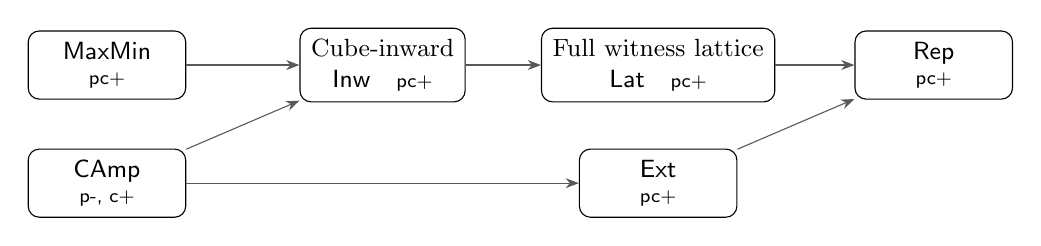
\begin{tikzpicture}[>=Stealth,
 box/.style={draw,rounded corners,align=center,minimum width=2cm,
             minimum height=.85cm,font=\small,inner sep=4pt},
 incl/.style={->,draw=black!65,thin}]
\node[box] (mm) at (0,0) {$\MaxMin$\\[-2pt]{\scriptsize\textsf{pc+}}};
\node[box] (camp) at (0,-1.5) {$\mathsf{CAmp}$\\[-2pt]{\scriptsize\textsf{p-, c+}}};
\node[box] (inw) at (3.5,0) {Cube-inward\\$\mathsf{Inw}$\quad{\scriptsize\textsf{pc+}}};
\node[box] (lat) at (7,0) {Full witness lattice\\$\mathsf{Lat}$\quad{\scriptsize\textsf{pc+}}};
\node[box] (rep) at (10.5,0) {$\Rep$\\[-2pt]{\scriptsize\textsf{pc+}}};
\node[box] (ext) at (7,-1.5) {$\mathsf{Ext}$\\[-2pt]{\scriptsize\textsf{pc+}}};
\foreach \a/\b in {mm/inw,camp/inw,inw/lat,lat/rep,camp/ext,ext/rep}
 \draw[incl] (\a)--(\b);
\end{tikzpicture}}
\caption{Refinements omitted from the structural overview.
Every arrow is a proved inclusion; no strictness is asserted.
The original adjacent comparisons and the added adjacent comparisons
remain undecided here. The symbol \textsf{?} means closure is not
established in this audit, not a proved failure or an assertion of
literature-wide openness. The classes in panel~(b) are defined in
\cref{def:atlas-witness-properties}; their inclusions and closure,
and the additional closure badges in panel~(a), are justified in
\cref{prop:atlas-witness-refinements,prop:atlas-refinement-minor-closure}.
No comparison of $\mathsf{Inw}$ or $\mathsf{Lat}$ with $\mathsf{Ext}$,
or of $\mathsf{HalfFrac}$ with $\mathsf E_k$, is asserted.
The $\mathsf{CAmp}\subseteq\mathsf{Ext}$ arrow follows from
\cref{prop:atlas-cube-chordal-complement}.}
\label{fig:allocation-refinements}
\end{figure}



\subsection{How many coordinates must be conditioned?}
\label{sec:auxiliary-hierarchy}

A second hierarchy measures the number of conditioned coordinates, rather
than the decomposition of the parent. For a displayed class
$C\subseteq\bits^X$, define
\[
 a(C)=\min\{|A|:C=M[A=\tau],\ M\subseteq\bits^{X\sqcup A}
                       \text{ maximum}\},\qquad
 \mathcal M_k=\{C:a(C)\le k\},
\]
with $a(C)=\infty$ if no parent exists. This is the minimum auxiliary
count studied in the earlier parent constructions \cite{MaxParents}.
Here the displayed coordinate set is retained, \emph{including constant
coordinates}. Unlike unrestricted $\MaxMin$ and the families $\mathcal P_k$,
this quantity is not invariant under adding or suppressing constants.
Thus the present hierarchy is one of coordinate classes, with this explicit
exception to the graph-comparison convention of the atlas.

\begin{proposition}[A strict hierarchy by auxiliary count]
\label{prop:auxiliary-hierarchy}
The definition of $\mathcal M_k$ is unchanged if the maximum parent is
required to use exactly $k$ auxiliary coordinates. Moreover
\[
 \mathcal M_0=\mathsf{Max},\qquad
 \mathcal M_0\subsetneq\mathcal M_1\subsetneq\mathcal M_2
 \subsetneq\cdots,\qquad
 \bigcup_{k\ge0}\mathcal M_k=\MaxMin.
\]
Each level is closed under projection, full reduction and cube complementation,
with empty complementary boundary cases allowed. Conditioning $j$ coordinates
maps $\mathcal M_k$ into $\mathcal M_{k+j}$; no fixed level is closed under
all conditionings. If $C\subsetneq\bits^n$ is nonempty, then
\begin{equation}\label{eq:auxiliary-complement-bound}
 a(C)\ \ge\ \operatorname{VC}(C)+\operatorname{VC}(C^c)+1-n.
\end{equation}
For every $m\ge0$, the active-coordinate class
\[
 F_m=\{00,01,10\}\times\bits^m
 \quad\text{satisfies}\quad a(F_m)=m.
\]
Thus the strict inclusions have explicit witnesses, even with no constant
coordinates present.
\end{proposition}
\begin{proof}
Let $M$ be a rank-$r$ maximum parent. If $r>0$, choose a maximum
rank-$(r-1)$ subclass $L\subseteq M$; if $r=0$, use $L=\varnothing$.
The nested expansion $(M\times\{0\})\cup(L\times\{1\})$ is maximum
of rank $r$. Marking its new coordinate zero keeps the original target
and adds one auxiliary. Repetition proves equivalence of ``at most'' and
``exactly,'' and the increasing-chain assertion. The union identity is
the definition of a maximum parent.

Project or fully reduce a visible coordinate of the parent to prove the
corresponding closure claims, retaining the old mark. Complementing a proper
parent retains that mark and gives the complementary target. A full target
has the allowed empty complement. Extra conditioning simply adds to the mark.

If a proper target on $n$ coordinates has a rank-$r$ parent on $n+k$
coordinates, that parent is proper. Its complement is maximum of rank
$n+k-r-1$, and has section $C^c$. Section monotonicity of VC dimension gives
\[
 \operatorname{VC}(C)\le r\le n+k-1-\operatorname{VC}(C^c).
\]
This proves \eqref{eq:auxiliary-complement-bound}.
For $F_m$, the two VC dimensions are $m+1$ and $m$, respectively,
since $F_m^c=\{11\}\times\bits^m$. With $n=m+2$ the bound gives
$a(F_m)\ge m$. The initial class $F_0$ is maximum of rank one.
The free-coordinate construction of \cref{prop:parent-free-coordinates}
adds the $m$ cube coordinates using at most $m$ auxiliaries, proving equality.
In particular $F_{k+1}\in\mathcal M_{k+1}\setminus\mathcal M_k$.

If some $\mathcal M_k$ were closed under all conditionings, it would
contain every section of every maximum class, since maximum classes lie
in $\mathcal M_k$. It would equal $\MaxMin$, contradicting strictness.
\end{proof}

The same witnesses show that $a(C)$ can grow under adding free coordinates,
while the least parent decomposition level, defined below, is unchanged
by \eqref{eq:parent-depth-cube}.
There is a separate constant-coordinate issue. For $m\ge0$,
\begin{equation}\label{eq:auxiliary-constant-example}
 a(\bits^m\times\{0\})=m,
 \qquad a(\bits^m)=0.
\end{equation}
Indeed the two complementary shores both have VC dimension $m$, so
\eqref{eq:auxiliary-complement-bound} gives the lower bound $m$.
Start with a singleton on one coordinate, a maximum rank-zero class,
and apply the free-coordinate construction to obtain the matching upper
bound. Suppressing constants before evaluating $a$ would define a different
invariant; in particular the displayed-cube complement law could not then
be imported without checking the change of ambient cube.

Fixing $k$ makes membership a finite problem. If $C$ has VC dimension $d$
and a rank-$r$ parent with $k$ auxiliaries, then
\[
 d\le r\le d+k.
\]
For the upper bound, when $r\ge k$ the full reduction of the parent on
all $k$ auxiliaries is maximum of rank $r-k$ and is contained in the marked
section; when $r<k$ the inequality is immediate. One can therefore examine
only finitely many ranks and classes on the fixed $n+k$ coordinates. This
is a finiteness statement, not an efficient algorithm. The earlier rank-free
MaxMin question asks whether $a(C)$ is finite for every ample $C$; it is not
settled by deciding any one fixed level.

\subsection{The complex of maximum projections}
\label{sec:maximum-projection-complex}

Ordinary shattering asks whether a projection is a full cube. One can instead
ask whether it is maximum at its own VC dimension. For a nonempty ample
class $C\subseteq\bits^X$, define its \emph{maximum-projection complex} by
\[
 \operatorname{MP}(C)=\{S\subseteq X:C|_S\text{ is maximum}\}.
\]
Here $C|_S$ means projection onto $S$, retaining its displayed coordinates.
The name distinguishes this notion from inclusion-maximal shattered sets.
Since projections of maximum classes are maximum, this is a simplicial
complex, and $\Sh(C)\subseteq\operatorname{MP}(C)$. Every singleton is
in $\operatorname{MP}(C)$, even if that coordinate is constant. Moreover
$\operatorname{MP}(C)=2^X$ if and only if $C$ itself is maximum.

\begin{proposition}[Maximum projections from the shattered complex]
\label{prop:maximum-projection-complex}
Put $\Delta=\Sh(C)$ and $\Delta|_S=\{T\in\Delta:T\subseteq S\}$.
Then
\begin{equation}\label{eq:maximum-projection-skeleton}
 S\in\operatorname{MP}(C)
 \quad\Longleftrightarrow\quad
 \Delta|_S=\{T\subseteq S:|T|\le d_S\}
 \text{ for some }0\le d_S\le |S|.
\end{equation}
If $S$ is a minimal nonface of $\operatorname{MP}(C)$ and $m=|S|$,
then $m\ge2$ and
\begin{equation}\label{eq:maximum-projection-obstruction}
 \Delta|_S=\{T\subseteq S:|T|\le m-2\}\ \cup\ \mathcal F,
 \qquad
 \varnothing\ne\mathcal F\subsetneq\binom{S}{m-1}.
\end{equation}
Conversely, \eqref{eq:maximum-projection-obstruction} makes $S$ a minimal
nonface. Every corresponding projection $C|_S$ belongs to
$\mathcal M_1\setminus\mathcal M_0$: it needs exactly one conditioned
coordinate in a maximum parent.
\end{proposition}
\begin{proof}
Projections preserve ampleness, and
$\Sh(C|_S)=\Delta|_S$. Hence $\lvert C|_S\rvert=\lvert\Delta|_S\rvert$. This equals the Sauer
bound at rank $d_S=\VC(C|_S)$ precisely when every subset of size at most
$d_S$ is present. This proves \eqref{eq:maximum-projection-skeleton}.

We prove the minimal-nonface assertion for any simplicial complex $\Delta$
containing the empty face. Suppose its restriction to $S$ is not the family
of all subsets up to some size, but every proper restriction is. At some
size $q$, there is both a present and an absent subset of $S$. The $q$-subsets
are connected by exchanges of one element. Along a path from a present set
to an absent one, two consecutive sets have different status and union of
size $q+1$. If $q\le m-2$, this union would be a proper restriction that
is already nonuniform, a contradiction. Thus mixed membership is possible
only at size $m-1$. A present $(m-1)$-set supplies faces at all smaller
sizes; since none of those sizes can have mixed membership, every smaller
set is present. An absent $(m-1)$-set excludes $S$. This proves
\eqref{eq:maximum-projection-obstruction}. Conversely, on every proper
subset the displayed family is either a full simplex or all subsets up to
size $m-2$, proving minimality.

Write $D=C|_S$, $t=|\mathcal F|$ and $q=m-t$. Ample complement duality
on the $m$ displayed coordinates states
\[
\Sh(D^c)=\{T\subseteq S:S\setminus T\notin\Sh(D)\}.
\]
Indeed, $T$ fails to be shattered by $D^c$ exactly when a complete
fibre with free coordinates $S\setminus T$ lies in $D$. This says that
$S\setminus T$ is strongly shattered by $D$, equivalently shattered
because $D$ is ample.
Consequently $\Sh(D^c)$ consists of the empty set and $q$ singleton
supports. The complement therefore has $q$ active coordinates, $t$ constant
coordinates, and $q+1$ words. On its active coordinates it is a maximum
rank-one class: its one-inclusion graph is a tree with every coordinate
appearing on exactly one edge. Here $q,t\ge1$.
To see the tree assertion directly, ampleness supplies an edge in every
active direction. Two distinct edges in the same direction would have tags
differing at another coordinate, shattering a pair and contradicting VC
dimension one. Thus there are exactly $q$ edges; the connected one-inclusion
graph on $q+1$ vertices is a tree.

This tree with its constants has an explicit one-auxiliary maximum parent.
Keep it in the zero shore of a new coordinate $a$. Attach an $a$-edge at
any tree vertex, and from its other endpoint attach a path that toggles each
of the $t$ constant visible coordinates once. The resulting tree uses all
$m+1$ coordinate directions exactly once, hence is maximum of rank one.
Its $a=0$ section is exactly $D^c$. Complementing this parent gives a
rank-$(m-1)$ maximum parent of $D$ with the same one-coordinate mark.
Since $D$ is nonmaximum, it cannot belong to $\mathcal M_0$.
\end{proof}

Equivalently, the projection-minimal nonmaximum ample classes are precisely
cube complements of rank-one maximum coordinate trees with at least one
active and at least one constant coordinate. This is a classification of
minimal failures of maximumity, not of failures of maximum ancestry.
Indeed all of these minimal failures already lie in $\mathcal M_1$.

Ampleness is essential for the skeleton test. The six-cycle
$\bits^3\setminus\{000,111\}$ shatters exactly the subsets of size at
most two, but it has six concepts rather than the seven required for a
rank-two maximum class. Its shattered complex alone therefore does not
certify maximumity without the ample hypothesis.

For an elementary example take $F_m=\{00,01,10\}\times\bits^m$, with
special coordinates $1,2$ and remaining set $Z$. Directly,
\[
 \Sh(F_m)=\{S:\{1,2\}\nsubseteq S\},\qquad
 \operatorname{MP}(F_m)=\Sh(F_m)\cup\{\{1,2\}\}.
\]
Thus the minimal nonfaces are exactly $\{1,2,z\}$ for $z\in Z$.
When $m=1$, $\operatorname{MP}(F_1)$ is the boundary of a triangle, whereas
$\Sh(F_1)$ omits the edge $\{1,2\}$. For arbitrary $m$, every minimal
bad projection needs one auxiliary, but the whole class needs $m$ by
\cref{prop:auxiliary-hierarchy}. Local one-auxiliary parents therefore
need not give a single one-auxiliary parent of the original class.

The complex has a limitation worth recording with its structural uses:
\eqref{eq:maximum-projection-skeleton} makes it determined entirely by
ordinary shattered supports. Every simplicial complex $\Delta$ is the
shattered complex of the downset class of its face indicators; that class
is ample and already belongs to $\MaxMin$. Therefore any
$\operatorname{MP}(C)$ arising from an ample class also arises from a
known maximum minor. It cannot by itself certify nonmembership in $\MaxMin$.
It can still organize maximum projections and their compatibility. If ranks
are needed, retain $d_S=\VC(C|_S)$ on its faces: bare complexes do not even
distinguish maximum classes of different ranks, all of which give $2^X$.

\subsection{The decomposition depth of a maximum parent}
\label{sec:parent-depth}

Having a maximum parent means exactly being a c-minor of a maximum
class, hence belonging to $\MaxMin$. The decomposition of that parent
is an additional requirement, distinct from the decomposition of its section. To compare them, for $k\ge0$ define
\[
 \mathcal P_k=\{M[A=\tau]\ne\varnothing:
                 M\text{ is maximum and }M\in\mathcal D_k\}.
\]
Write $\lambda(C)=\min\{k:C\in\mathcal P_k\}$, with value $\infty$
when the set is empty. Also put $\kappa(C)=\infty$ for nondismantlable
classes, extending the earlier definition of intrinsic decomposition depth.
No bound on the number of auxiliary coordinates is imposed.

\begin{proposition}[Parent depth and feasible ranks]
\label{prop:parent-depth-hierarchy}
For every $k\ge0$,
\[
 \mathcal P_k\subseteq\mathcal D_k\cap\MaxMin,\qquad
 \mathcal P_k\subsetneq\mathcal P_{k+1},\qquad
 \bigcup_{k\ge0}\mathcal P_k=\mathcal P_D.
\]
Each $\mathcal P_k$ is closed under nonempty coordinate sections,
projections and full reductions. It is unchanged by adding or suppressing
constant coordinates. The family $\mathcal P_0$ is complement closed,
with the empty boundary case allowed; no $\mathcal P_k$ with $k\ge1$
is complement closed. Moreover
\[
 \kappa(C)\le\lambda(C),
 \qquad \lambda(M)=\kappa(M)\quad\text{for maximum }M.
\]
For $C\in\mathcal P_D$, let $h_k(C)$ be its least maximum-parent rank
with parent in $\mathcal D_k$, or $\infty$ if none exists, and let
$h_D(C)$ be its least dismantlable maximum-parent rank. Then the feasible
ranks at level $k$ are exactly the integers at least $h_k(C)$, whenever
$h_k(C)$ is finite. The sequence $h_k(C)$ is nonincreasing, and
\[
 h_k(C)=h_D(C)\quad\text{if }k\ge\max\{h_D(C)-1,0\}.
\]
\end{proposition}
\begin{proof}
Sections preserve $\mathcal D_k$, so every eligible parent gives the first
inclusion and $\kappa(C)\le\lambda(C)$. A maximum class is its own
parent, proving equality of the depths there. Every dismantlable parent
belongs to some finite $\mathcal D_k$, proving the union formula.
The polygon maximum $C_{2k+5}$ has depth $k+1$ by
\cref{prop:polygon-decomposition}; it therefore witnesses the strict
inclusion at level $k$.

Additional conditioning can be retained as a mark on the original parent.
Projection or full reduction in a visible coordinate commutes with that
mark and preserves maximumity and $\mathcal D_k$, unless its output is
empty. This proves the asserted closure laws. The constant-coordinate
construction preceding \cref{prop:parent-free-coordinates} uses only
maximum predecessors and face avoidance, both of which preserve the
supplied level $k$ by \cref{prop:decomposable-maximum-sequences}.
For complements, if the parent is proper, complement it and keep its mark.
The resulting parent is maximum; for $k=0$ it remains in $\mathcal D_0$
by complement closure of $\Rper$. A full parent gives a full section and
an empty complementary boundary case. In contrast, the maximum polygon
class $H_{2k+5}$ has depth one whereas its complement has depth $k+1$.
For $k\ge1$ this disproves complement closure of $\mathcal P_k$.

Suppose $M\in\mathcal D_k$ is a supplied proper rank-$r$ parent on $N$
coordinates. Choose a rank-$(r+1)$ maximum $U\supseteq M$ in the same
level using \cref{prop:decomposable-maximum-sequences}. On a fresh
coordinate $a$, the nested expansion
\[
 (M\times\{0\})\cup(U\times\{1\})
\]
is maximum of rank $r+1$ and lies in $\mathcal D_k$. Marking $a=0$
retains the old target. If $M$ is full, use the full cube on $N+1$
coordinates with the same new mark. Iteration realizes every larger rank.
Monotonicity in $k$ follows from $\mathcal D_k\subseteq\mathcal D_{k+1}$.
Finally every dismantlable class of VC dimension $r\ge1$ lies in
$\mathcal D_{r-1}$ \cite{RecursiveClasses}: along a corner peeling,
the uniquely lost shattered support has size at most $r$, and supplies
a shedding face of that size in the Yang complex. Rank-zero parents
are singletons. Applying this bound to a parent of rank $h_D(C)$ proves
the stabilization assertion.
\end{proof}

\begin{figure}[htbp]
\centering
\resizebox{\textwidth}{!}{%
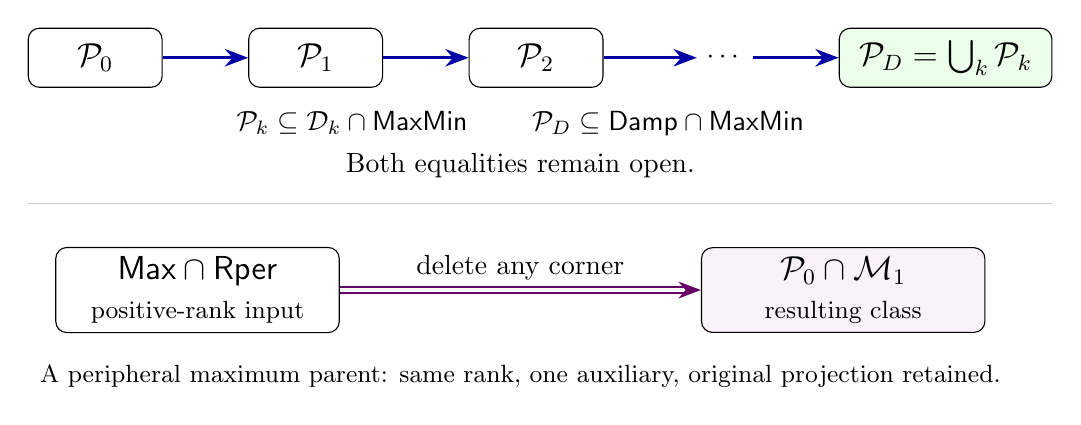
\begin{tikzpicture}[>=Stealth,
 box/.style={draw,rounded corners,align=center,minimum height=.75cm,
 minimum width=1.7cm,font=\large},
 strict/.style={->,draw=blue!65!black,line width=1.2pt},
 operation/.style={->,draw=violet!80!black,double,double distance=1.5pt,
 line width=.7pt}]
\node[box] (p0) at (0,3.4) {$\mathcal P_0$};
\node[box] (p1) at (2.8,3.4) {$\mathcal P_1$};
\node[box] (p2) at (5.6,3.4) {$\mathcal P_2$};
\node (dots) at (8,3.4) {$\cdots$};
\node[box,fill=green!8,minimum width=2.7cm] (pd) at (10.8,3.4)
 {$\mathcal P_D=\bigcup_k\mathcal P_k$};
\draw[strict] (p0)--(p1);
\draw[strict] (p1)--(p2);
\draw[strict] (p2)--(dots);
\draw[strict] (dots)--(pd);
\node[align=center] at (5.4,2.3)
 {$\mathcal P_k\subseteq\mathcal D_k\cap\MaxMin$
 \qquad $\mathcal P_D\subseteq\Damp\cap\MaxMin$\\[3pt]
 Both equalities remain open.};
\draw[black!20] (-.85,1.55)--(12.15,1.55);
\node[box,minimum width=3.6cm] (input) at (1.3,.45)
 {$\Max\cap\Rper$\\{\small positive-rank input}};
\node[box,fill=violet!5,minimum width=3.6cm] (output) at (9.5,.45)
 {$\mathcal P_0\cap\mathcal M_1$\\{\small resulting class}};
\draw[operation] (input)--node[above,font=\normalsize]
 {delete any corner} (output);
\node[align=center,font=\small] at (5.4,-.65)
 {A peripheral maximum parent: same rank, one auxiliary, original projection retained.};
\end{tikzpicture}}
\caption{Maximum-parent classes and a construction between them.
The class $\mathcal P_k$ consists of sections of maximum parents in
$\mathcal D_k$, whereas $\mathcal M_k$ bounds the number of auxiliary
coordinates. Blue single arrows are proved strict inclusions
(\cref{prop:parent-depth-hierarchy}); the purple double arrow applies an
operation to each input (\cref{prop:peripheral-corner-parent}). It does
not assert $\Rper\subseteq\MaxMin$. The union $\mathcal P_D$ uses
arbitrary dismantlable maximum parents.}
\label{fig:parent-hierarchy-construction}
\end{figure}

The cube-factor construction of \cref{prop:parent-free-coordinates} also
has an exact converse. For every $m\ge0$,
\begin{equation}\label{eq:parent-depth-cube}
 \lambda(C\times\bits^m)=\lambda(C),\qquad
 h_k(C\times\bits^m)=h_k(C)+m,
\end{equation}
with $\infty+m=\infty$. The construction gives the upper inequalities.
Conversely, full reduction in the $m$ displayed free coordinates recovers
$C$ and lowers the rank of any maximum parent by exactly $m$, retaining
its decomposition level. This proves the rank lower bound; section closure
proves the depth lower bound.

Thus decomposition depth and parent rank are related but distinct quantities.
The polygon examples already give $\lambda(H_{2m+1})=1$ and
$\lambda(H_{2m+1}^c)=m-1$: even among maximum classes with dismantlable
complements, complementary parent depth has no bound in terms of parent
depth alone. The following comparisons remain open here:
\[
 \mathcal P_k\stackrel{?}{=}\mathcal D_k\cap\MaxMin,
 \qquad \mathcal P_D\stackrel{?}{=}\Damp\cap\MaxMin.
\]
The first asks whether a maximum parent can always be replaced by one
of the section's own decomposition level. It is stronger than merely
asking whether that section has some maximum parent. Neither comparison
follows from the strict hierarchy above.

\subsection{Compatible predecessors and dismantlable deletion parents}
\label{sec:compatible-deletion-parents}

A useful distinction is whether a construction merely supplies a maximum
parent or also controls its decomposition. The face-avoidance construction
can be made compatible with inclusions, and the minimum-section deletion
construction preserves dismantlability under explicit hypotheses.

Fix an ordered list $D=(j_1,\ldots,j_q)$ of distinct coordinates and a
pattern $\tau\in\bits^D$. For any class $C$, including the empty class,
define $L_{D,\tau}(C)$ on the same ambient coordinates as follows.
For $D=\varnothing$ the output is empty. Otherwise put
$j=j_1$, $D'=D\setminus\{j\}$ and $I=\partial_jC$, and set
\[
 L_{D,\tau}(C)=
 (I\times\{1-\tau_j\}_j)\cup
 (L_{D',\tau|_{D'}}(I)\times\{\tau_j\}_j).
\]
This fixes the coordinate choices in the usual face-avoidance construction
\cite[Theorem~\textnormal{Face avoidance}]{MaxParents}.

\begin{proposition}[Compatible face avoidance]
\label{prop:monotone-predecessors}
The operator $L=L_{D,\tau}$ satisfies
\[
 L(C)\subseteq C,\qquad L(C)[\tau]=\varnothing,
 \qquad L(C\cap E)=L(C)\cap L(E).
\]
In particular it preserves inclusions. If $C$ is maximum of rank
$0\le r\le q$, its image is maximum of rank $r-1$, where the empty
class has formal rank $-1$. Nonempty outputs preserve each
$\mathcal D_k$, and preserve dismantlability.
\end{proposition}
\begin{proof}
Induct on the length of the coordinate list. Both lifts of
$\partial_jC$ lie in $C$, and the second output shore is contained in
the first by induction. The first shore disagrees with $\tau$ at $j$;
the second avoids its remaining pattern. Full reduction commutes with
intersection, so the intersection identity follows by taking intersections
separately in the two disjoint shores and applying induction.

A singleton has empty image. For positive rank $r$, the two output
shores are maximum of ranks $r-1,r-2$ on one fewer coordinate, with
an empty second shore when $r=1$. Pascal's identity gives the
rank-$(r-1)$ Sauer cardinality. No $r$-support avoiding $j$ is
shattered in the first shore, and no $r$-support containing $j$ is
shattered at height $\tau_j$. This proves maximumity. Finally full
reduction and nested expansion preserve $\mathcal D_k$ and
$\Damp$; an empty shore is handled by constant extension.
\end{proof}

For example, let $B\subseteq A$ be maximum classes of ranks $r-1,r$,
and let $v\in A\setminus B$ be a corner with support $J$, of size $r$.
With $\tau=v|_J$, the same ordering of $J$ gives
\[
 P=L_{J,\tau}(A),\qquad K=L_{J,\tau}(B),
 \qquad K\subseteq B\cap P.
\]
Thus the intersection contains a maximum rank-$(r-2)$ subclass,
without requiring a common recursive decomposition of $A$ and $B$.
The corner cube $F$ satisfies $L_{J,\tau}(F)=F\setminus\{v\}$,
so monotonicity also gives $F\setminus\{v\}\subseteq P$.

\begin{proposition}[Dismantlable parents for minimum-section deletions]
\label{thm:dismantlable-minimum-deletion}
Let $M\subseteq\bits^X$ be maximum of rank $r$, and let $J\subseteq X$
have size $1\le q\le r$. Suppose a pattern $p\in\bits^J$ has smallest
section $M[p]=\partial_JM=S$, and put
\[
 C=M\setminus(S\times\{p\}).
\]
If $M,C\in\mathcal D_k$, then $C$ has a maximum parent of rank $r$
in $\mathcal D_{\max(k,r-1)}$ with exactly $r+1-q$ auxiliary coordinates.
This auxiliary count is optimal among rank-$r$ parents.
In particular, if $M$ and $C$ are dismantlable, then
$C\in\mathcal P_D$.
\end{proposition}
\begin{proof}
We prove that the minimum-section construction
\cite[Theorem~\textnormal{Deleting a smallest coordinate section}]{MaxParents}
preserves the stated decomposition level. Write $\ell=\max(k,r-1)$.
Choose a maximum predecessor $S'\subseteq S$ in $\mathcal D_\ell$;
use the empty class when $S$ has rank zero. Such a predecessor exists
by \cref{prop:monotone-predecessors}. The prescribed-section step of
that construction produces a maximum rank-$(r-1)$ class $A\subseteq M$
with
\[
 A[p]=S',\qquad
 S\times(\bits^J\setminus\{p\})\subseteq A.
\]
Its recursion on $q$ has the form
$A=(I\times\{1-p_j\}_j)\cup(K\times\{p_j\}_j)$,
where $I=\partial_jM$ and $K\subseteq I$ is the corresponding
prescribed-section predecessor for the remaining block.
The recursion shows that both $A$ and
$A_{\rm off}=A\setminus(S'\times\{p\})$ belong to
$\mathcal D_\ell$, allowing an empty latter class: for $q=0$ they
are $S'$ and $\varnothing$, while for $q>0$ their second shores
are respectively $K$ and $K_{\rm off}$, both contained in $I$.
It also proves the displayed punctured-cube containment for
$A_{\rm off}$, by induction in the $p_j$ shore and by
$S\times\bits^J\subseteq M$ in the other shore.

Set $D_0=(S\setminus S')\times\{p\}$ and introduce a new coordinate $a$.
The existing construction proves that
\[
 N=((M\setminus D_0)\times\{0\}_a)
       \cup((A\cup D_0)\times\{1\}_a)
\]
is maximum of rank $r$, with new smallest section $S'$ at the
pattern $(p,0)$ on $J\cup\{a\}$. For the decomposition, start from
\[
 E=(C\times\{0\}_a)\cup(A_{\rm off}\times\{1\}_a).
\]
Since $A_{\rm off}\subseteq C$, this is a nested expansion in
$\mathcal D_\ell$. Its $p$-section on $J$ is empty, and each other
$J$-section contains $S\times\bits^{\{a\}}$.
The missing $p$-section of $N$ is
\[
 Z=(S'\times\{0\}_a)\cup(S\times\{1\}_a),
\]
a nested class in $\mathcal D_\ell$. It lies in every other
$J$-section of $E$. Adding it is a defining attachment on $q$
coordinates, so $N\in\mathcal D_\ell$, since $q\le r\le\ell+1$.

The induction also needs the deletion of the new smallest section to
remain in that level. Removing $S'$ at $(p,0)$ from $N$ leaves the
same base $E$ with $p$-section $S\times\{1\}_a$. This is another
valid attachment on $J$, proving that requirement.
Repeat the construction: the marked block grows by one and its
minimum rank falls by one at each step. After $r-q+1$ steps the
minimum is empty, and conditioning all new coordinates to zero
recovers exactly $C$. Every attachment block has size at most $r$,
so the same $\ell$ works throughout. The fixed-rank lower bound
is the one in the cited minimum-section theorem. If both inputs
are dismantlable, choose a common finite $k$ to obtain the last claim.
\end{proof}

\begin{proposition}[Peripheral deletion of a smallest section]
\label{prop:peripheral-minimum-deletion}
Under the minimum-section hypotheses of
\cref{thm:dismantlable-minimum-deletion}, if $M$ is peripheral, then $C$
is peripheral. Consequently $C$ has a maximum parent of rank $r$ in
$\mathcal D_{r-1}$ with $r+1-q$ auxiliary coordinates, and
$C\in\mathsf R_{\rm per}\cap\mathcal P_D$.
\end{proposition}
\begin{proof}
Induct on $|X|$. For a full cube, reflect $p$ to the all-one pattern;
the deletion is a downset, hence peripheral. Otherwise choose a nested
peripheral decomposition $M=A\times\{0\}_j\cup B\times\{1\}_j$,
where $B\subseteq A$ have ranks $r-1$ and $r$ respectively.
If $j\in J$, put $K=J\setminus\{j\}$. The alternative $p_j=0$ would give
\[
 S=\partial_K B\subseteq\partial_K A\subseteq A[p|_K]=S,
\]
contradicting the respective reduction ranks $r-q$ and $r-q+1$.
Thus $p_j=1$ and $B[p|_K]=\partial_KB$. For nonempty $K$, apply
induction to this deletion in $B$ and retain $A$; the shores remain
nested. For empty $K$, the whole smaller shore disappears, leaving a
constant extension of $A$.

If $j\notin J$, conditioning at $j$ commutes with full reduction on $J$.
Both shores therefore inherit the smallest-section equality. Delete the
same $J$-pattern in each shore; induction preserves peripheral structure,
and the two deletions preserve containment. If $q>r-1$, the specified
section of $B$ is empty, so $B$ is unchanged. This proves deletion
closure, allowing empty shores as recursive boundary cases. Apply
\cref{thm:dismantlable-minimum-deletion} with $k=0$ for the parent assertion.
\end{proof}

When the smallest section has positive rank, the stronger conclusion
$C\in\mathcal P_0$ remains open. Peripheral structure of the deletion
does not by itself ensure a peripheral maximum parent.

For a corner deletion $C=M\setminus\{v\}$ one has $q=r$ and obtains
one auxiliary coordinate. In this case assuming $C\in\mathcal D_k$
alone suffices: adding back the corner is a singleton-site attachment
on its $r$-support, so $M\in\mathcal D_{\max(k,r-1)}$.
Thus every dismantlable corner deletion of a maximum class has a
same-rank dismantlable maximum parent. When $M$ is proper, the deletion
still has VC dimension $r$ and is nonmaximum, so rank $r$ and one
auxiliary are both optimal. A full-cube deletion is already maximum
of rank $r-1$, so this optimality assertion does not apply to it.
These results control the decomposition of existing maximum-parent
constructions. They do not prove $\mathcal P_D=\Damp\cap\MaxMin$,
nor do they in general ensure a peripheral parent at level zero.
For corner deletion, however, that stronger conclusion holds as follows.

\begin{proposition}[Peripheral parents after a prescribed corner deletion]
\label{prop:peripheral-corner-parent}
Let $M\subseteq\bits^X$ be a peripheral maximum class of positive rank $r$,
and let $v$ be any corner. Then $M\setminus\{v\}$ is peripheral and has
a peripheral maximum parent $N\subseteq\bits^{X\cup\{a\}}$ of rank $r$
with
\[
 \pi_XN=M,\qquad N[a=0]=M\setminus\{v\}.
\]
Thus the deletion belongs to $\mathcal P_0\cap\mathcal M_1$.
If $M$ is proper, rank $r$ and one auxiliary coordinate are both optimal.
\end{proposition}
\begin{proof}
We choose the ordering of the corner support $J$ so that the usual parent
\[
 N=((M\setminus\{v\})\times\{0\}_a)
       \cup((L_{J,v|_J}(M)\cup\{v\})\times\{1\}_a)
\]
is peripheral. Maximumity and the displayed projection and section follow
from the one-corner case of the minimum-section construction. The proof
retains a nested coordinate of $M$, rather than requiring the auxiliary
coordinate to have nested shores.

First, every corner of a rank-$r$ maximum class has support size $r$.
Deleting it removes exactly that support from the shattered family.
Removing a support of size less than $r$ would leave a containing
$r$-support shattered, contradicting downward closure.

Induct on $|X|$, allowing a rank-zero singleton as a boundary input:
its predecessor is empty, and its parent is the singleton at auxiliary
height one, with empty zero section. If $M$ is a full cube of positive
rank, any ordering gives $L(M)=M\setminus\{v\}$ and
$N=\bits^{X\cup\{a\}}\setminus\{(v,0)\}$.
Both the deletion and this parent become downsets after reflection,
so are peripheral.

Otherwise choose a peripheral split, reflecting its coordinate if necessary:
\[
 M=(A\times\{0\}_j)\cup(B\times\{1\}_j),\qquad B\subseteq A.
\]
The shores $A,B$ are peripheral maximum classes of ranks $r,r-1$.
Write $w$ for the projection of $v$ away from $j$.
If $j\notin J$, the corner has no $j$-neighbor, so $w\in A\setminus B$
and is a corner of $A$ with support $J$.
If $j\in J$, the corner must be in the smaller shore: otherwise it would
be a corner of the rank-$r$ class $A$ with support $J\setminus\{j\}$,
of size $r-1$. In that case $w$ is a corner of $B$ with support
$J\setminus\{j\}$.

In the first case, use the order of $J$ supplied inductively for $A,w$.
The operator $L=L_{J,v|_J}$ commutes with conditioning on $j\notin J$:
this follows recursively because full reductions in other coordinates
commute with that conditioning. The $j$-shores of $N$ are therefore
\[
 N_A=((A\setminus\{w\})\times\{0\}_a)
       \cup((L(A)\cup\{w\})\times\{1\}_a),\qquad
 N_B=(B\times\{0\}_a)\cup(L(B)\times\{1\}_a).
\]
Induction makes $N_A$ peripheral, and $N_B$ is a nested peripheral
expansion. Since $B\subseteq A\setminus\{w\}$ and
$L(B)\subseteq L(A)$, we have $N_B\subseteq N_A$.
Thus $N$ is peripheral. The deletion likewise has nested peripheral
shores $A\setminus\{w\}$ and $B$.

In the second case, put $j$ first, followed by the order supplied
inductively for $B,w$. If $L'$ denotes the remaining operator, the
$j$-shores of $N$ are
\[
 N_A=(A\times\{0\}_a)\cup(B\times\{1\}_a),\qquad
 N_B=((B\setminus\{w\})\times\{0\}_a)
       \cup((L'(B)\cup\{w\})\times\{1\}_a).
\]
The first is a nested peripheral expansion; the second is the peripheral
parent from induction. Both auxiliary shores of $N_B$ lie in $B$, so
$N_B\subseteq N_A$. The deletion has nested peripheral shores $A$ and
$B\setminus\{w\}$, allowing an empty smaller shore. This completes
both inductions. For proper $M$, the deletion remains of VC dimension
$r$ and is nonmaximum, which gives the two optimality assertions.
\end{proof}

By complement closure, every ample one-vertex extension of a peripheral
maximum class also belongs to $\mathcal P_0$. For an original rank-$r$
maximum class on $n$ coordinates with $r\le n-2$, complementing the
parent of the complementary corner deletion gives a peripheral maximum
parent of rank $r+1$ with one auxiliary. If the extension is the full
cube, it is already maximum. Neither statement proves corner-deletion
closure for arbitrary nonmaximum peripheral classes, or supplies a
maximum parent for every peripheral class. Peripheral preservation for
minimum-section deletions with positive-dimensional minima remains open.

\subsection{Dismantlability of the complement}
\label{sec:complement-dismantlable}

It is useful to separate the two requirements in $\mathcal B$. Write
\[
 \mathsf{coDamp}=\{C\in\Amp:C^c\in\Damp\cup\{\varnothing\}\}.
\]
The complement is taken in the displayed coordinate cube. Thus
$\mathcal B=\Damp\cap\mathsf{coDamp}$. This is a complementary family,
not a proposed subclass of $\Damp$.

\begin{proposition}[Complementary dismantlability and representation]
\label{prop:complement-dismantlable}
The family $\mathsf{coDamp}$ is closed under nonempty sections, projections
and full reductions, and under adding or suppressing constant coordinates.
Neither $\Damp$ nor $\mathsf{coDamp}$ contains the other, and
\[
 \mathcal B\subsetneq\mathsf{coDamp}\subsetneq\Amp,
 \qquad \MaxMin\not\subseteq\Damp\cup\mathsf{coDamp}.
\]
The following open comparisons are equivalent in pairs:
\begin{align*}
 \Damp\subseteq\mathsf{Ext}
 &\quad\Longleftrightarrow\quad\mathsf{coDamp}\subseteq\Rep,\\
 \Damp\subseteq\MaxMin
 &\quad\Longleftrightarrow\quad\mathsf{coDamp}\subseteq\MaxMin.
\end{align*}
The first pair is a necessary consequence of the second. No converse
implication is established here.
\end{proposition}
\begin{proof}
Complementation commutes with sections and exchanges projection and full
reduction: $(\pi_i C)^c=\partial_i(C^c)$ and
$(\partial_i C)^c=\pi_i(C^c)$. Apply the corresponding closure properties
of $\Damp$. For a constant extension, the complement of $C\times\{0\}$
has nested shores $C^c$ and the full cube. Both are dismantlable, allowing
an empty smaller shore, so their nested expansion is dismantlable.

Let $H$ be Hall's nondismantlable maximum class and put $K=H^c$, the
known dismantlable maximum complement. Then
$H\in\mathsf{coDamp}\setminus\Damp$ and
$K\in\Damp\setminus\mathsf{coDamp}$. This proves incomparability and
both strict signs. For the stronger non-containment, put $C=H\times K$,
which belongs to $\MaxMin$ by product closure. Fixing the second factor
to a word of $K$ gives the nondismantlable section $H$ of $C$.
Fixing the first factor to a word of $H$ gives the section $H$ of $C^c$.
Thus neither $C$ nor $C^c$ is dismantlable.

Every dismantlable class has a representation map. Therefore
\eqref{eq:cube-extension-complement} makes $\Damp\subseteq\mathsf{Ext}$
equivalent to representability of every complement of a dismantlable class.
This is precisely $\mathsf{coDamp}\subseteq\Rep$, with harmless empty
boundary cases. Complement closure of $\MaxMin$ proves the second
 equivalence, and $\MaxMin\subseteq\mathsf{Ext}$ gives the implication
between the pairs.
\end{proof}

\begin{figure}[ht]
\centering
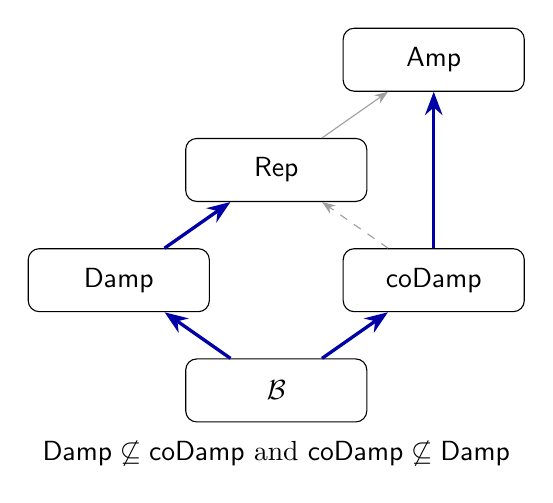
\begin{tikzpicture}[>=Stealth,
 box/.style={draw,rounded corners,minimum width=23mm,minimum height=8mm},
 strict/.style={->,blue!65!black,line width=1.2pt},
 incl/.style={->,gray!75},open/.style={->,gray!75,dashed}]
 \node[box] (b) at (0,0) {$\mathcal B$};
 \node[box] (d) at (-2,1.4) {$\Damp$};
 \node[box] (c) at (2,1.4) {$\mathsf{coDamp}$};
 \node[box] (r) at (0,2.8) {$\Rep$};
 \node[box] (a) at (2,4.2) {$\Amp$};
 \draw[strict] (b)--(d);\draw[strict] (b)--(c);
 \draw[strict] (d)--(r);\draw[open] (c)--(r);
 \draw[incl] (r)--(a);\draw[strict] (c)--(a);
 \node[align=center] at (0,-.8) {$\Damp\not\subseteq\mathsf{coDamp}$ and
 $\mathsf{coDamp}\not\subseteq\Damp$};
\end{tikzpicture}
\caption{Complementary dismantlability. The dashed arrow is open.
Thick blue arrows are strict inclusions. Hall's complementary maximum
classes witness the two non-containments.}
\label{fig:complement-dismantlable}
\end{figure}

There is also a useful product rule that does not assume product closure
of all of $\mathsf{coDamp}$.
\begin{proposition}[A product with both sides dismantlable]
\label{prop:complement-dismantlable-product}
If $C\in\mathsf{coDamp}$ and $D\in\mathcal B$ are on disjoint
coordinate sets, then $C\times D\in\mathsf{coDamp}$.
\end{proposition}
\begin{proof}
Put $P=C^c\subseteq\bits^X$ and $Q=D^c\subseteq\bits^Y$. The
complement of the product is
\[
 U=(P\times\bits^Y)\cup(\bits^X\times Q).
\]
The ample prefixes in a dismantling order of $D$, after complementation,
give a corner-deletion sequence from $\bits^Y$ down to $Q$. Choose a
corner-deletion sequence for $P$. If its current remainder is $P_t$ and
its next corner is $p$, keep every other row intact and run the relative
sequence $\bits^Y\searrow Q$ in the $p$-row of
$(P_t\times\bits^Y)\cup(\bits^X\times Q)$.

At a deletion $(p,y)$, necessarily $y\notin Q$. Its incident directions
in $X$ are exactly those of $p$ in $P_t$; its directions in $Y$ are those
of $y$ in its current row. Let $F,G$ be the two incident corner cubes.
The product cube $F\times G$ is present: its $p$-row is in the current
row, and every other row over $F$ is still full. Thus this is a valid
corner deletion. After finishing the row, the same expression for the
remainder holds with $P_t\setminus\{p\}$ in place of $P_t$. At the end
only $\bits^X\times Q$ remains, which is dismantlable by product closure
of $\Damp$. The empty-complement cases give empty stages of this proof.
The original product is ample, so it belongs to $\mathsf{coDamp}$.
\end{proof}

The extra condition $D\in\Damp$ is used to obtain the relative deletion
sequence to $D^c$. Merely knowing that $D^c$ is dismantlable does not
supply that sequence. General product closure of $\mathsf{coDamp}$ is
not established here.

A precise representation problem underlies the first open comparison in
\cref{prop:complement-dismantlable}. Here a corner's support means all its
incident coordinate directions, which span its unique maximal cube.
\begin{lemma}[Representation after deleting a corner]
\label{lem:corner-representation-deletion}
Let $E$ be ample and let $v$ be a corner with support $T$. Then
$E\setminus\{v\}$ has a representation map if and only if some
representation map $r$ of $E$ satisfies $r(v)=T$.
\end{lemma}
\begin{proof}
Deleting the corner removes exactly $T$ from the shattered family.
Consequently a map assigning $T$ to $v$ restricts to a representation
map of the deletion. Conversely, extend any map of the deletion by
$v\mapsto T$. No other word of $E$ agrees with $v$ on $T$: an isometric
path to such a word would have to start in a direction outside $T$,
contradicting the definition of $T$. Thus $T$ separates $v$ from every
other word, proving all new nonclashing conditions and the assertion.
\end{proof}

The members of $\mathsf{coDamp}$ are exactly the ample classes reachable
from their full cube by corner deletions: complementing that sequence
gives ample prefixes of a dismantlable class, and conversely.
Therefore it would suffice to prove that a represented member of
$\mathsf{coDamp}$ can always choose a map assigning any specified corner
its full support. The lemma makes this assertion equivalent to
$\mathsf{coDamp}\subseteq\Rep$, by induction from the full cube.
The assertion allows all values of a supplied map to change; preserving
particular values is a stronger requirement. Nor is assigning the full
corner support the same as assigning the empty support at a prescribed
root. No existence theorem for this map choice is claimed here.

\begin{proposition}[Deleting a corner with at most two directions]
\label{prop:small-corner-map-repair}
Let $D$ be ample with a representation map $r$, and let $v$ be a corner
with support $J$, where $|J|\le2$. By at most three exchanges of labels
inside its corner cube, one can obtain a representation map $r'$ with
$r'(v)=J$. Every label outside that cube remains unchanged. Consequently
$D\setminus\{v\}$ has a representation map, allowing an empty output.
The VC dimension of $D$ is unrestricted.
\end{proposition}
\begin{proof}
For any ample representation map, the cube obtained by toggling an arbitrary
subset of $r(x)$ at $x$ lies in $D$; moreover exactly one endpoint of an
$i$-edge has $i$ in its label \cite[Corollary~6.7 and Theorem~6.8]{CCMW}.
We first note a safe exchange. If adjacent words $u,w=u^i$ carry labels
$A,A\cup\{i\}$, with $i\notin A$, exchanging their labels preserves
representation. The support bijection is unchanged and the label at $u$
only increases. If $w$ clashed with a third word $z$ after its label shrank,
then $w,z$ would agree on $A\cup r(z)$. Old nonclashing with $u$ forces
$i\in r(z)$ and $z(i)=w(i)$, which makes $w,z$ clash already before the
exchange. This contradiction proves the claim.

The corner's trace on $J$ is unique in $D$, by the isometry argument in
\cref{lem:corner-representation-deletion}. Thus its corner cube $Q$ is the
unique positioned $J$-cube, and the owner $p$ of label $J$ lies in $Q$ by
the outgoing-cube property. Also $r(v)\subseteq J$. If $u=v^i$ points
toward $v$, so $i\in r(u)$, its label contains no coordinate $a\notin J$:
otherwise its outgoing cube would contain $v^a$, contrary to the corner
condition. We use this restriction on the incoming neighbors below.

A zero-dimensional corner is a singleton. For $J=\{i\}$, either $v$
already owns $J$, or the two labels on its edge are $\varnothing,\{i\}$;
one safe exchange suffices.
For $J=\{i,j\}$, write $a=v^i$, $b=v^j$, $w=v^{\{i,j\}}$.
If $r(v)=J$, stop. Up to interchanging $i,j$, the remaining cases and
exchanges are
\[
\begin{array}{c|c|c|l}
 r(v)&p&\text{other required labels}&\text{successive exchanges}\\\hline
 \{i\}&b& & (v,b)\\
 \{i\}&w&r(b)=\{j\}&(w,b),\ (b,v)\\
 \varnothing&a&r(b)=\{j\}&(v,b),\ (v,a)\\
 \varnothing&w&r(a)=\{i\},\ r(b)=\{j\}&(v,a),\ (w,b),\ (v,b).
\end{array}
\]
Here is why the table is exhaustive and its required labels are exact.
If $r(v)=\{i\}$, edge consistency excludes $p=a$. The neighbor $b$
points toward $v$, so its label is contained in $J$ and contains $j$;
unless $p=b$, it must be $\{j\}$. If $r(v)=\varnothing$, both neighbors
point toward $v$ and have labels contained in $J$. Any such neighbor
that does not own $J$ must therefore carry its corresponding singleton.
These observations give every row of the table. In each listed exchange,
the two labels differ exactly by the direction of their edge, so the safe
exchange applies globally. The last label at $v$ is $J$. Finally delete
$v$ and use \cref{lem:corner-representation-deletion}.
\end{proof}

The proof repairs a supplied map; it does not assume that arbitrary labels
can be retained. Its geometric argument proves that labels outside the
small corner cube can remain fixed. This yields a concrete step for the
complementary induction: if $B\in\mathsf{Ext}$ and $B\cup\{v\}$ is a
corner addition with corner support $S$ satisfying $|X\setminus S|\le2$,
then $B\cup\{v\}\in\mathsf{Ext}$. Indeed, the complementary deletion
has support $X\setminus S$ and is covered by the proposition; the map on
$B$ extends by assigning $v\mapsto S$. Repeated deletions of corners with
at most two directions preserve representation maps. General complementary
peelings can have larger corners, so this does not establish
$\Damp\subseteq\mathsf{Ext}$.

\subsection{Learning spaces and their minor closure}

\begin{proposition}[Learning spaces, daisy cubes, and maximum ancestry]
\label{prop:learning-daisy-maxmin}
Every finite learning-space graph and every daisy cube belongs to
$\Rper\cap\RAmp$, and therefore to $\MaxMin$. Moreover,
\[
 \Cl_{pc}(\mathsf{Learn})=\Cl_c(\mathsf{Learn})
 \subseteq\Rper\cap\RAmp\subseteq\Damp\cap\MaxMin.
\]
For a learning space on $n\ge1$ coordinates with $q$ inclusion-minimal
missing consistent partial labelings, the construction in \cite{MaxParents}
gives a maximum parent of VC dimension $n$ with at most $q+2n$ auxiliary
coordinates. The zero-coordinate singleton needs none.
\end{proposition}
\begin{proof}
The realizations and quantitative parent construction are
\cite[the explicit downset realization and
Theorem~\textnormal{Maximum parents of learning spaces}]{MaxParents}.
For downsets, the stronger Theorem~\textnormal{Exact parent parameters
for two monotone shores} also gives optimal parent parameters.
The realization proofs use strict linear inequalities to realize
exactly the allowed orthants; a bounded perturbation supplies the generic
arrangement giving the maximum parent. The preceding lemma in that source
checks exclusion of forbidden closed orthants as well as preservation of
allowed witnesses, so the passage to a generic arrangement is justified.

For the recursive inclusion, both coordinate sections of a down-set are
down-sets. A singleton class is the recursion base. Otherwise, in a
learning space choose a feasible singleton $\{e\}$.
Union closure gives $\mathcal F_{e=0}\subseteq\mathcal F_{e=1}$.
Both sections are accessible and union closed: for the one-section, union
a feasible prefix chain with $\{e\}$ and omit its repeated $e$-step.
Induction gives $\Rper$ membership, as in the same source. Coordinate
reorientation handles graphs without a prescribed root; unused coordinates
are harmless. Finally, projection closure of learning spaces gives
$\Cl_{pc}=\Cl_c$, and minor closure of $\Rper$ and $\RAmp$ gives the
asserted containment of the closure.
\end{proof}

The qualitative convex-realizability theorem is already supplied by
Chalopin--Chepoi--Knauer \cite[Theorem~26]{CCKGeometry}, via coordinate
complementation between antimatroids and convex geometries. The source
\cite{MaxParents} gives a direct proof and the explicit maximum-parent bound.
These are unrestricted finite-class theorems. They settle two natural
subclasses of the $\Rper\subseteq\MaxMin$ question, while that whole
inclusion and $\Damp\subseteq\MaxMin$ remain open. Their convex
realizability uses hyperplane sign regions in an open convex domain,
not a claim that every antimatroid is Euclidean point-set convexity.


\begin{proposition}[The learning-space minor closure]\label{prop:learning-ideal-closure}
The following is an exact generative description:
\[
 \Cl_{pc}(\mathsf{Learn})=\Cl_c(\mathsf{Learn})=\mathsf{Icg}.
\]
Every member is obtained by conditioning one new coordinate of a learning
space. Its full normalized positive coefficient space is Euclidean.
\end{proposition}
\begin{proof}
Complementation turns a lower ideal of a convex geometry into an upper
ideal $I$ of a learning space $L$. Define the marker extension
\[
 \widehat L=(L\times\{0\})\cup(I\times\{1\}).
\]
It is union closed: a union involving a marked member lies above a member
of $I$ in $L$, hence remains in $I$. It is accessible: a marked member can
delete its marker, and unmarked members use accessibility of $L$.
Conditioning the marker to one gives $I$.

For the reverse containment, the small-scale coefficient test in
\cite[Theorems~2--3]{CoefficientScaling} is preserved under projection and
conditioning and vanishes exactly on upper ideals of learning spaces. It
vanishes on every learning space, proving the reverse inclusion. That source
also constructs the unique largest ambient learning space on the same coordinates from the positive
minimal missing patterns. Its scaling-interval theorem proves the Euclidean
full-space assertion. The qualitative realizability of convex-geometry ideals
is the earlier theorem of \cite[Theorem~26]{CCKGeometry}.
\end{proof}

Median classes belong to $\mathsf{Icg}$ by
\cite[Corollary~25]{CCKGeometry}. This inclusion is strict:
$\bits^3\setminus\{111\}$ is a daisy cube, hence belongs to
$\mathsf{Icg}$, but the majority of $110,101,011$ is its missing word.
Daisy cubes also belong to $\mathsf{Icg}$: complementing a downset gives
an upper ideal of the full cube, which is a learning space. The inclusion
$\mathsf{Icg}\subseteq\RAmp$ is strict. The 17-concept example in
\cite{CoefficientScaling} has a Euclidean coefficient space but a nonconvex
logarithmic coefficient domain, whereas every member of $\mathsf{Icg}$ has
a convex logarithmic domain in the coefficient ratios.

\begin{center}
\small
\begin{tabular}{@{}lccc>{\raggedright\arraybackslash}p{.38\textwidth}@{}}
\toprule
Family & p-closed & c-closed & pc-closed & Result of pc closure\\
\midrule
Ample, median, daisy, ACC & yes & yes & yes & The same family\\
$\Rper$, $\Damp$, $\RAmp$ & yes & yes & yes & The same family\\
$\mathcal D_k$, $\mathcal B$, $\mathsf{coDamp}$ & yes & yes & yes & The same family\\
$\Rep$, $\Frac$, $\mathsf{Ext}$, $\MaxMin$ & yes & yes & yes & The same family\\
$\mathcal P_D$, $\mathcal P_k$, $\mathsf U_k$, $\mathsf P_k$
 & yes & yes & yes & The same family\\
$\mathsf{Inw}$, $\mathsf{Lat}$ & yes & yes & yes & The same family\\
$\mathsf{BFrac}$, $\mathsf M$, $\mathsf{HalfFrac}$
 & yes & yes & yes & The same family\\
$\mathsf{CAmp}$ & no & yes & no & Not identified; contained in $\Damp$\\
$\mathsf{Pos}_k$ ($k\ge3$) & yes & ? & ? & Not identified here\\
$\mathsf E_k$ ($k\ge1$) & ? & ? & ? & Not assessed here\\
Maximum; each fixed $\mathcal M_k$ & yes & no & no & $\MaxMin$\\
Learning spaces & yes & no & no & $\mathsf{Icg}=\Cl_c(\mathsf{Learn})$\\
Convex-geometry ideals & yes & yes & yes & The same family\\
Signed bouquets $\mathsf{Bouq}^{\pm}$ & yes & yes & yes & The same family\\
Tree-like & yes & no & no & All of $\PCube$\\
\bottomrule
\end{tabular}
\end{center}

Here the symbol \textsf{?} means that this audit makes no assertion,
not a proved counterexample or a claim of literature-wide openness.
The new allocation and whole-witness entries follow from
\cref{prop:atlas-witness-refinements,prop:atlas-refinement-minor-closure}.
The fixed-$\mathcal M_k$ rows retain all ambient coordinates.
The two width notations $\mathsf P_k$ and $\mathcal P_k$ refer,
respectively, to chunk peelings of the class and decomposition of a
maximum parent; they are not interchangeable.

Ample minor closure and the representation/corner facts are from \cite{CCMW,Partition};
the daisy, cover-recursive, and learning-space rows are from
\cite{Daisy,Cover,Survey,MaxParents}. Median closure follows from majority closure and
isometry. Realizable closure follows by dropping a hyperplane for projection
and intersecting the open convex domain with the selected open halfspaces
for conditioning; ampleness is preserved separately. Tree-like projection
closure follows by induction on its construction: projecting an old coordinate
in \eqref{eq:peripheral} projects both $B$ and $S$, while projecting the new
coordinate recovers $B$.

\subsection{Intersection-closed ample classes and signed bouquets}
\label{sec:signed-bouquets}

Intersection closure singles out a classical family with explicit allocation
maps. It is larger than the convex-geometry ideals already appearing in the
atlas. This section consolidates that distinction and the relevant recent
results; the longer operator proofs remain in their original notes.

\begin{definition}[Bouquets and their signed version]
\label{def:atlas-signed-bouquets}
A \emph{bouquet of convex geometries} on a finite set $E$ is a family
$C\subseteq2^E$ such that $\varnothing\in C$, $A\cap B\in C$ for all
$A,B\in C$, and
\[
 A,B\in C,\quad A\subsetneq B
 \quad\Longrightarrow\quad
 A\cup\{e\}\in C\text{ for some }e\in B\setminus A.
\]
The last property is local one-element extendability. These are also called
\emph{conditional antimatroids}. A bouquet containing $E$ is a convex
geometry. Define
\[
 \mathsf{Bouq}^{\pm}
 :=\{C\in\Amp:\text{some }C\mathbin\triangle r
                  \text{ is intersection-closed}\},\qquad
 C\mathbin\triangle r:=\{A\mathbin\triangle r:A\in C\}.
\]
The superscript records coordinate flips, not ambient cube complementation.
\end{definition}

\begin{proposition}[Characterization and minor closure]
\label{prop:atlas-bouquet-characterization}
For a nonempty intersection-closed family containing $\varnothing$,
ampleness is equivalent to local one-element extendability. Consequently
$\mathsf{Bouq}^{\pm}$ is exactly the signed-coordinate class of bouquets,
with constant coordinates suppressed as usual. It is p-closed and c-closed,
and hence pc-closed. For an ample $C$, equivalently
\[
 C\in\mathsf{Bouq}^{\pm}
 \quad\Longleftrightarrow\quad
 \exists r\in C\quad
 \operatorname{maj}(u,v,r)\in C\quad(u,v\in C),
\]
where $\operatorname{maj}$ denotes coordinatewise majority.
\end{proposition}
\begin{proof}
An ample class is isometric. A Hamming geodesic between comparable members
adds their differing elements one at a time, giving local extendability.
The converse is the classical ampleness theorem for conditional antimatroids
\cite[\S3.2.4]{CCMW}; the equivalent bouquet axioms are
\cite[\S2.5]{CCKGeometry}.

For any nonempty intersection-closed family $H$, its total intersection
$m=\bigcap H$ is a member. Flipping the coordinates of $m$, which are
constant one on $H$, gives an intersection-closed family containing zero.
Thus an initially arbitrary witnessing flip can be changed to an actual
word $r\in C$. In the orientation with $r=0$, the displayed majority
condition is precisely closure under intersection, proving the equivalence.

Projection commutes with intersection. A conditioning is also
intersection-closed: the meet of two words agreeing with the fixed pattern
still agrees with it. Both operations preserve ampleness. Coordinate flips
restrict to the remaining coordinates; newly constant one coordinates can
be normalized by the total-intersection argument. This proves both closure
claims, including conditionings that discard the original root.
\end{proof}

\begin{example}[Why the full ground set is not required]
\label{ex:atlas-bouquet-star}
On three coordinates, $\{\varnothing,\{1\},\{2\},\{3\}\}$ is a bouquet
and a daisy cube, but is not a convex geometry on that ground set. It is
nevertheless an ideal of the full Boolean convex geometry. Thus omission
of the full set alone does not distinguish bouquets from convex-geometry
ideals; \cref{prop:atlas-bouquet-position} gives a genuine separation.
\end{example}

\paragraph{Recognition by forbidden partial patterns.}
A \emph{minimally missing pattern} $(S,a)$ has
$a\notin C|_S$, while every proper restriction of $a$ occurs. For a proposed
flip $r$, intersection closure is equivalent to
\begin{equation}\label{eq:atlas-bouquet-horn}
 \bigl|\{i\in S:r_i=a_i\}\bigr|\le1
 \qquad\text{for every minimally missing }(S,a).
\end{equation}
Indeed, agreement at two positions lets two witnesses for the proper
restrictions have a majority with $r$ realizing the missing pattern.
Conversely, if $w=\operatorname{maj}(u,v,r)$ is absent, choose a minimally
missing restriction of $w$. The nonempty sets of positions where $u$ and
$v$ disagree with it are disjoint, and $r$ agrees with it on both sets,
contradicting \eqref{eq:atlas-bouquet-horn}.
The pairwise prohibitions are a 2-SAT formula in the bits of $r$. This is
the classical \emph{renamable-Horn} condition, not a new recognition
theorem; see \cite[\texttt{lem:horn-test}]{BouquetProjection}.
The 2-SAT size is measured in the supplied minimally missing patterns,
not in an unspecified implicit description of $C$.

\paragraph{Explicit maps on both complementary classes.}
Work in an intersection-closed orientation $H$ on the full original
ground set $E$. Put
\[
 \begin{aligned}
 \rho(v)&=\{i\in v:v\setminus\{i\}\in H\},&
 \downarrow H&=\{a:a\subseteq v\text{ for some }v\in H\},\\
 c(a)&=\bigcap\{v\in H:a\subseteq v\}
       &&(a\in\downarrow H).
 \end{aligned}
\]
The classical representation map is $v\mapsto\rho(v)$; its whole downward
cube is present by intersection closure. Deleting words in decreasing
cardinality gives the classical corner peeling
\cite[Proposition~4.9]{CCMW}. The closure fibers satisfy
\begin{equation}\label{eq:atlas-bouquet-fibers}
 c^{-1}(v)=[\rho(v),v]
 :=\{a:\rho(v)\subseteq a\subseteq v\}.
\end{equation}
If $c(a)=v$, omitting a removable element contradicts minimality of $c(a)$.
Conversely, if $\rho(v)\subseteq a\subseteq v$ but $c(a)\subsetneq v$,
a geodesic from $c(a)$ to $v$ ends at a lower neighbor $v\setminus\{i\}$,
forcing $i\in\rho(v)\setminus c(a)$, a contradiction.

The recent complementary construction in
\cite[\texttt{thm:closure-completion}]{BouquetCompletion} assigns, on
$K=2^E\setminus H$,
\begin{equation}\label{eq:atlas-bouquet-complement}
 r_K(a)=
 \begin{cases}
 E\setminus a,&a\notin\downarrow H,\\
 (E\setminus c(a))\cup(a\setminus\rho(c(a))),
       &a\in\downarrow H\setminus H.
 \end{cases}
\end{equation}
It is an ordinary representation map made of actual whole cubes. More
strongly, it is the remaining-neighbor map of a corner peeling: process
closure fibers by increasing $|v|$, process each
$[\rho(v),v]\setminus\{v\}$ by decreasing $|a|$, and finally process
$2^E\setminus\downarrow H$ by increasing $|a|$.
The cited proof verifies every selected cube and every omitted neighboring
direction. It retains original constants and allows the empty complement.
This is an author-proved recent result, with external priority unresolved;
it is not attributed to the classical primal-map theorem.

\begin{proposition}[Position in the atlas]
\label{prop:atlas-bouquet-position}
With the preceding complementary-completion input,
\[
 \mathsf{Icg}\subsetneq\mathsf{Bouq}^{\pm}
 \subseteq\mathcal B\subsetneq\mathsf{Ext},\qquad
 \mathsf{Bouq}^{\pm}\not\subseteq\RAmp.
\]
In particular, signed bouquets are corner-peelable and representable.
\end{proposition}
\begin{proof}
An ideal of a convex geometry is closed under intersection, since the
intersection is a closed set below either member of the ideal. It is ample
by \cite[\S2.5]{CCKGeometry}, so signed ideals lie in
$\mathsf{Bouq}^{\pm}$. The two peeling constructions give
$\mathsf{Bouq}^{\pm}\subseteq\mathcal B$.
The strict inclusion $\mathcal B\subsetneq\mathsf{Ext}$ is already proved
in \cref{prop:maxmin-neighbors}.

The 26-set bouquet of \cite{NonrealizableBouquet} has no affine-convex
realization in any finite dimension. Every signed convex-geometry ideal
is realizable by \cite[Theorem~26]{CCKGeometry}, and realizability is
invariant under coordinate flips. This proves both the first strictness
and the displayed noncontainment. That same bouquet has a certified
maximum parent; it is not a non-$\MaxMin$ example.
\end{proof}

\paragraph{Attaching a cube without assuming a daisy intersection.}
The complementary construction extends beyond a single bouquet.
\begin{proposition}[A clamped cube on a signed bouquet]
\label{prop:atlas-bouquet-cube-attachment}
Let $B\in\mathsf{Bouq}^{\pm}$ be nonempty on the original frame $E$, and
let $C=Q(z,S)$ be a positioned cube. Suppose its coordinate clamp
\[
 c_C(b)|_S=b|_S,\qquad c_C(b)|_{E\setminus S}=z|_{E\setminus S}
\]
satisfies $c_C(B)\subseteq B$. Then $B\cup C\in\mathsf{Ext}$.
Every supplied ordinary representation map on $B$ extends to $B\cup C$
without changing its old rooted-cube columns; an ordinary map on
$(B\cup C)^c$ can be constructed simultaneously. Cyclic supplied maps
are allowed. No chordality or daisy-intersection hypothesis is required.
\end{proposition}
\begin{proof}
Flip coordinates to make $B$ intersection-closed. Clamps commute with
this change of coordinates. The compatible-completion theorem
\cite[\texttt{thm:horn-gluing}]{CubeComplementCompletion} constructs a full
actual-cube basis, retains the supplied primal basis, and supplies the
entire complementary basis. Translate its two maps back to the original
frame, retaining all constants.
\end{proof}
The union need not itself be a signed bouquet. In particular this is an
attachment theorem, not a closure law for $\mathsf{Bouq}^{\pm}$, nor an
iteration rule for arbitrary unions of differently oriented bouquets.

\paragraph{Operator characterization and remaining question.}
For $g_0=(1,0)^t$ and $g_1=(1,-1)^t/\sqrt2$, let $P_C$ be the orthogonal
projection onto the span of the tensors $\bigotimes_{i\in E}g_{v_i}$,
$v\in C$. CP's author theorem
\cite[\texttt{thm:classification}]{BouquetProjection} says, for isometric
$C$, that $P_C$ is entrywise nonnegative in some real orthonormal product
basis exactly when a flip makes $C$ intersection-closed. A product basis
chooses an orthonormal basis separately at each coordinate. Entrywise
nonnegativity is stronger than positive semidefiniteness. This is an
algebraic characterization of the same family, not evidence that all ample
classes admit such a basis. Its full spectral proof is not independently
certified by this atlas consolidation.

The question whether every signed bouquet has a finite maximum parent
remains open in the campaign. The ideal subclass has such parents, and the
nonrealizable 26-set example does too. Neither the explicit two-shore maps
nor the operator characterization supplies parents for all bouquets.
No comparison with all of $\Rper$ or all of $\mathsf{CAmp}$ is asserted.


\subsection{Maximum ancestry is a conditioning-closure problem}

\begin{proposition}[Maximum sections]\label{prop:max-sections}
Projections of maximum classes are maximum. Consequently,
\[
 \MaxMin=\Cl_c(\Max).
\]
Equivalently, $C\in\MaxMin$ precisely when $C=M[D=\tau]$ for a finite
maximum class $M$ on the original coordinates together with an auxiliary set
$D$, and one fixed auxiliary word $\tau$. No projection is needed in this
certificate.
\end{proposition}
\begin{proof}
For a maximum VC-$d$ class on $n$ coordinates with $0<d<n$, split at one
coordinate and put $U=C_i^0\cup C_i^1$, $I=C_i^0\cap C_i^1$.
Then $\VC(U)\le d$ and $\VC(I)\le d-1$. The latter follows because any
support shattered by $I$, together with $i$, is shattered by $C$.
Moreover $|C|=|U|+|I|$. The two Sauer bounds sum, by Pascal's identity,
to the maximum cardinality of $C$. Equality for their sum forces equality
in each, so $U$ is maximum. For $d=0$ the projection is a singleton, and
for $d=n$ it is a full cube. Repeating proves projection closure.
Now apply \cref{prop:operators}. This is the maximum-section certificate
proved in the source module of \cite{MaxSections}.
\end{proof}

\begin{example}[Conditioning a maximum class need not stay maximum]
Let $K=\{\varnothing,\{1\},\{2\},\{3\}\}$ and put
\[
 M=K\cup\{A\cup\{z\}:A\in K\}
   \cup\{\{1,2\},\{1,3,z\},\{2,3,z\}\}.
\]
Every pair is shattered and no triple is shattered: the old triple misses
111, and for a triple $\{i,j,z\}$ the trace 11 on $i,j$ occurs with only
one value of $z$. Thus $M$ is maximum of VC dimension two on four coordinates,
with $11$ concepts. Its $z=0$ conditioning is
$C=K\cup\{\{1,2\}\}$, which has five concepts, VC dimension two, and
three active coordinates. It is ample but not maximum, since the Sauer
bound there is seven. This is the nonmaximum-section example in
\cite{Partition}.
\end{example}

The certificate is already an exact generative description of $\MaxMin$
in terms of maximum parents. It is not yet an intrinsic test that avoids
searching over parents of unbounded auxiliary dimension. The open equality
$\MaxMin=\Amp$ asks whether that construction covers all ample classes.
Geometric realizability supplies a substantial positive subfamily: bounded
convex witnesses and a sufficiently small generic perturbation give a maximum
arrangement class with the required prescribed section \cite{Geometry}.

\subsection{Closure and core give opposite answers for tree-like classes}

\begin{proposition}[The tree-like contrast]\label{prop:tree-like}
Within $\PCube$,
\[
 \Cl_c(\mathsf{TreeLike})=\Cl_{pc}(\mathsf{TreeLike})=\PCube,
 \qquad
 \Core_c(\mathsf{TreeLike})=\Core_{pc}(\mathsf{TreeLike})=\Rper.
\]
\end{proposition}
\begin{proof}
For the closure assertion, embed an arbitrary partial cube $H$ in $Q_n$.
The full cube is tree-like. Its peripheral expansion along $H$ is tree-like
as well, and conditioning the new coordinate to one gives $H$. This is
\cite[Remark on nonheredity]{Cover}. The core assertions are precisely the
convex-subgraph and pc-minor characterizations in that paper: every such
minor is tree-like exactly when the parent lies in $\Rper$. The
convex-subgraph characterization is already \cite[Proposition~5.6]{Polat};
\cite{Cover} identifies it with the recursive class and proves pc-minor closure.
\end{proof}

Thus sequential tree-like partial cubes themselves do not all lie in $\Amp$.
The cover-recursive paper is about a hereditary core, whereas the MaxMin
program is about a closure. Treating both as the same closure question would
lose their principal distinction.

Learning spaces provide a second warning. Their projections remain learning
spaces, but a conditioning can be the three-leaf star, which has no learning
root \cite[Proposition on the minor profile]{Learning}. Therefore the original
family has a p-obstruction problem; a pc-obstruction problem would instead
study the convex-geometry ideal class identified in
\cref{prop:learning-ideal-closure}. Root-preserving conditioning is a
third, pointed question, not unrestricted c-closure.

\section{Two boundaries of ampleness}\label{sec:obstructions}

\subsection{Minimal non-ample classes as a family in their own right}
\label{sec:minimal-nonample}

A class is \emph{minimal non-ample under conditioning} when it is non-ample
and every proper nonempty conditioning is ample. Because ampleness is
c-closed, it suffices to check one-coordinate conditionings. This is exactly
the minimality studied in \cite{MNA}, not minimality under deletion of concepts.
That paper proves that these classes are antipodal and, with at least three
concepts, are exactly the tope classes of non-free simple uniform oriented
matroids. In the two-concept case they are antipodal pairs, with parallel
coordinates in the oriented-matroid interpretation.

Write $\mathcal N=\Obs_c(\Amp)$ in the universe of nonempty concept
classes. This family belongs beside the inclusion diagram, on the outside
of $\Amp$: its members are the first failures of ampleness under
conditioning. It is a natural object of study independently of any
particular subclass of ample classes. Neither conditioning nor projection
preserves $\mathcal N$: a proper conditioning is ample, and projecting to
one coordinate gives a full edge. The class itself is included when taking
its minor closure, so a closure of $\mathcal N$ contains both non-ample and
ample objects.

There are two complementary descriptions already in the YangDim manuscript.
Its algebraic description identifies minimal non-ampleness with the Yang
complex being Buchsbaum but not Cohen--Macaulay
\cite[Theorem on the Buchsbaum characterization]{MNA}. Here the Yang complex
has one vertex for each realized coordinate literal $(i,b)$ and one facet
$\{(i,x_i):i\in E\}$ for each concept $x$. Conditioning corresponds to
taking a literal link. Thus the algebraic condition says that every nonempty
face link is Cohen--Macaulay whereas the whole complex is not.
The combinatorial description, for at least three concepts, is an
isometrically and irredundantly embedded antipodal partial cube that is not a cube and whose
proper convex antipodal
subgraphs are hypercubes \cite[Classification theorem]{MNA}. An antipodal
subgraph contains the opposite of each of its vertices in its own active
coordinates. The classification identifies these graphs with the non-free
simple uniform-oriented-matroid tope graphs. A combinatorial study here can
therefore build on a structural classification that already exists.
For a two-concept antipodal pair on at least two coordinates, simplifying
the parallel coordinates produces the ample edge $Q_1$. Thus simplification
does not preserve non-ampleness; the rank-one case must be retained separately.

The projection theorem gives a particularly useful connection to pc-minors.
For such a class on $n$ coordinates with VC dimension $k$, every one-coordinate
conditioning is maximum of VC dimension $k-1$. Its projection onto $t$
coordinates is:
\begin{center}
\begin{tabular}{@{}ll@{}}
\toprule
Number retained & Projected class\\
\midrule
$t\le k$ & The full $t$-cube\\
$t=k+1$ & A $(k+1)$-cube with two antipodes removed\\
$t>k+1$ & Another conditioning-minimal non-ample class of VC dimension $k$\\
\bottomrule
\end{tabular}
\end{center}
This is \cite[Theorem on the structure of a minimal non-ample class]{MNA}.
It explains how a rich c-minimal family reduces to a simpler pc-minimal one.
The two operations are displayed in \cref{fig:nonample-operations}; its
arrows describe operations on an individual class, rather than inclusions
between families.

\begin{figure}[htbp]
\centering
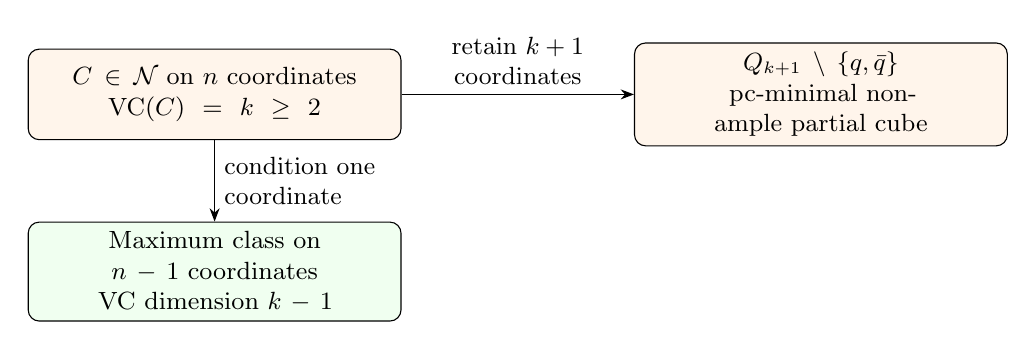
\begin{tikzpicture}[>=Stealth,
 box/.style={draw,rounded corners,align=center,text width=4.5cm,
             minimum height=1.15cm,font=\small}]
\node[box,fill=orange!8] (n) at (0,0)
 {$C\in\mathcal N$ on $n$ coordinates\\$\VC(C)=k\ge2$};
\node[box,fill=orange!8] (pc) at (7.7,0)
 {$Q_{k+1}\setminus\{q,\bar q\}$\\pc-minimal non-ample partial cube};
\node[box,fill=green!6] (m) at (0,-2.25)
 {Maximum class on $n-1$ coordinates\\VC dimension $k-1$};
\draw[->] (n)--node[above,align=center,font=\small]
 {retain $k+1$\\coordinates} (pc);
\draw[->] (n)--node[right,align=left,font=\small]
 {condition one\\coordinate} (m);
\end{tikzpicture}
\caption{The c-minimal non-ample family connects maximum classes and the
pc-obstruction basis of ampleness. The rank-one antipodal pairs are treated
separately in \cref{ex:ambient}. Projection can be the identity when
$n=k+1$.}
\label{fig:nonample-operations}
\end{figure}

Among partial cubes, the pc-obstructions to ampleness are exactly
\[
 \Obs_{pc}^{\PCube}(\Amp)
 =\{Q_n\setminus\{x,\bar x\}:n\ge3\},
\]
as recalled with its recognition source in \cite{Daisy,Partition}.

\begin{example}[A c-minimal class that is not pc-minimal]\label{ex:cycle}
The isometric eight-cycle has cyclically ordered vertices
\[
 0000,1000,1100,1110,1111,0111,0011,0001.
\]
Every one-coordinate conditioning is a four-vertex path with three distinct
edge directions, hence is maximum of VC dimension one. The whole cycle is
non-ample: it shatters two-coordinate sets but contains no square. It is
therefore c-minimal non-ample. Projecting away the first coordinate gives
\[
 \{000,100,110,111,011,001\}=Q_3\setminus\{010,101\},
\]
a non-ample six-cycle. Thus the eight-cycle is not pc-minimal.
\end{example}

\begin{example}[The ambient universe changes the basis]\label{ex:ambient}
The class $\{00,11\}$ is non-ample and all its proper nonempty p- and
c-minors are ample singletons or edges. It is pc-minimal among concept
classes, but its one-inclusion graph is disconnected, so it is excluded
from $\PCube$. Likewise $\{000,111\}$ is c-minimal and projects to
$\{00,11\}$. An obstruction table for arbitrary concept classes must
therefore retain the rank-one cases; the partial-cube table starts at $n=3$.
\end{example}

\subsection{A combinatorial study and its relation to maximum ancestry}
\label{sec:nonample-study}

The algebraic manuscript remains the source for its classification,
homological, and resolution results. A possible complementary study in
PartialCubes would develop ways to construct and manipulate the same objects
using coordinate halves, graph convexity, and extensions. Antipodality makes
one concrete starting point available. For a chosen coordinate, write
\[
 C=(A\times\{0\})\cup(\bar A\times\{1\}),
 \qquad \bar A=\{\bar a:a\in A\}.
\]
Every member of $\mathcal N$ has this form, with $A$ maximum. This is a
necessary description; an arbitrary maximum $A$ need not give a member of
$\mathcal N$. The constructive question is to determine which compatibility
conditions on $A$ and its coordinate faces ensure minimal non-ampleness,
and how those conditions behave when a coordinate is added or projected
away. The intended output would be an effective construction or extension
theorem with soundness and recovery, useful beyond a finite census.

For $0<d<n-1$, where $d=\VC(A)$, the exact condition is now known.
The double is c-minimal non-ample precisely when $A$ is obtained by fixing
one sign in a uniform oriented matroid, by the classification in \cite{MNA}.
By the intrinsic one-fixed-sign test in the CompressionSchemes reservoir
\cite[Corollary \textnormal{Intrinsic test for a one-fixed-sign parent}]{Partition},
this holds if and only if $A\cap\bar A$ and $\bits^E\setminus(A\cup\bar A)$
are minimal non-ample of VC dimensions $d$ and $n-d-1$. The open part is
therefore the construction calculus: coordinate extensions and recovery.

Before treating this as a new contribution, compare the proposed operations
with uniform-oriented-matroid extensions and the pseudogeometric realization
results already in \cite{MNA}. The abstract classification, maximum-half
theorem, projection trichotomy, and complement duality are established
inputs. The added value would have to lie in the construction calculus or
its applications, not in restating those results with graph terminology.
The accompanying source inventory records this as a research direction;
it does not add a second submission to the publication queue.

\begin{example}[Maximum halves need compatibility]\label{ex:maximum-halves}
Let $A=\{000,100,010,001\}$. This is maximum of VC dimension one:
it shatters each singleton and no pair, and has $1+3$ concepts.
The class $(A\times\{0\})\cup(\bar A\times\{1\})$ consists of two
disjoint three-leaf stars, since $A\cap\bar A=\varnothing$ gives no edge
in the new direction. More directly, conditioning its first old coordinate
to zero gives $\{000,100,010,111\}$. This class shatters its first two
coordinates but contains no square on them, so it is non-ample.
Thus the antipodal union of two maximum halves need not be c-minimal
non-ample. The compatibility requirement is substantive even in this
small example.
\end{example}

There is also a direct reason to place the YangDim and MaxMin results next
to one another. Recall $\mathcal N=\Obs_c(\Amp)$, with the stated
ambient convention. Its members have maximum one-coordinate conditionings.
Since $\MaxMin$ is c-closed, all their proper conditionings lie in
$\MaxMin$, so they are c-minimal outside $\MaxMin$. Conversely, a nonample
c-minimal nonmember of $\MaxMin$ contains a c-minimal non-ample conditioning,
which is itself outside $\MaxMin$; minimality forces equality. Thus
\begin{equation}\label{eq:maxmin-c-boundary}
 \Obs_c(\MaxMin)\setminus\Amp=\mathcal N.
\end{equation}
In the partial-cube universe the rank-one disconnected classes are omitted.
For pc-minors the corresponding source theorem is
\begin{equation}\label{eq:maxmin-pc-boundary}
 \Obs_{pc}^{\PCube}(\MaxMin)
 =\{Q_n^{--}:n\ge3\}\ \sqcup\ \mathcal B_{\max},
 \qquad \mathcal B_{\max}\subseteq\Amp,
\end{equation}
where the ample family $\mathcal B_{\max}$ is unknown and may be empty
\cite{Partition}. In particular, $\MaxMin=\Amp$ if and only if
$\mathcal B_{\max}=\varnothing$. Equations \eqref{eq:maxmin-c-boundary}
and \eqref{eq:maxmin-pc-boundary} describe different operation-dependent
boundaries of the same class.

This common nonample pc-boundary is not automatic for every subclass of
$\Amp$. To retain all $Q_n^{--}$ as minimal obstructions, that subclass
must contain their proper minors, including singly punctured cubes.
For example, $Q_3$ minus a vertex is not median: three neighbors of the
missing vertex have that vertex as their coordinatewise majority. One must
check this hypothesis before importing the same obstruction decomposition
into a different row of the atlas.

\input{sections/single_operation_obstructions}

\section{Where the papers fit}\label{sec:papers}

The following table separates each paper's mathematical role from its
remaining research and review obligations.

\small
\begin{longtable}{@{}>{\raggedright\arraybackslash}p{.23\textwidth}
 >{\raggedright\arraybackslash}p{.34\textwidth}
 >{\raggedright\arraybackslash}p{.35\textwidth}@{}}
\toprule
Source & Mathematical role & Current scope and next preparation step\\
\midrule\endhead
Daisy cubes \cite{Daisy}
& Complete generative pc-obstruction basis.
& Both soundness and exhaustive recovery are proved. Closest to submission;
final author and submission preparation remain.\\[5pt]
Cover recursion \cite{Cover}
& Largest c- and pc-closed subclass of sequential tree-like graphs; complete
coordinate-state test for its pc basis.
& A full membership criterion and validated source/evidence packages are
available. A simpler intrinsic generator and final scholarly review remain.\\[5pt]
Gluing \cite{Gluing}
& General shelling composition and relative-peeling tests; transfers suitable
minimal pairs $(A,K)$ to forbidden pc-minors.
& A reusable tool paper. The exposition and internal proof review are complete;
independent scholarly review and author submission decisions remain.\\[5pt]
Corner-peelable ample campaign \cite{AmpleCampaign}
& Reductions, structural constraints, constructions, and quantitative bounds
for ample pc-minimal failures.
& Full intrinsic generation remains open. The extracted note \cite{AmpleCorners}
certifies corner theorems in small dimension and an order-$267$ cornerless class.\\[5pt]
Learning spaces \cite{Learning,Survey}
& Projection preservation, failure under conditioning, valid-root tests,
and p-minimal nonmember constructions.
& Infinite construction families are proved, not a complete basis.
Standalone article extracted; nine proof inputs are shared with the survey.
Priority comparison and independent reading remain.\\[5pt]
Minimal non-ample classes \cite{MNA}
& c-minimal boundary of ampleness; uniform-OM classification and projection
trichotomy; algebraic and dual-realization consequences.
& The YangDim manuscript contains both algebraic results and a combinatorial
classification. A complementary construction/extension study in PartialCubes
is scoped in \cref{sec:nonample-study}; no separate paper is yet claimed.\\[5pt]
Maximum ancestry and representation maps \cite{Partition,MaxSections}
& MaxMin, its construction operations and obstruction decomposition;
pc-minor descent of representation maps.
& MaxMin $=$ Amp and universal representation maps remain open. The
results are consolidated by theorem family, with located review evidence
for every numbered statement in the CompressionSchemes campaign register.\\[5pt]
Recursive decomposition and complementary peeling
\cite{RecursiveClasses,RecursiveClosure,OrientationClasses}
& The classes $\mathcal D_1$ and $\mathcal B$, strict intermediate
inclusions, minor/product closure, and the orientation description of
$\mathcal B$.
& Structural theory and restricted parent constructions. Both inclusions
into $\MaxMin$ remain open. \Cref{prop:polygon-decomposition} proves
$\mathcal B\not\subseteq\mathcal D_1$; the opposite inclusion remains open.\\[5pt]
Geometric realization \cite{Geometry,MaxParents}
& Realizable ample classes have maximum parents; median, daisy and learning-space
classes have explicit realizations. The learning-space parent bound is quantitative.
& A proved supporting note. It gives ancestry, not just a representation map.
No independent novelty or submission assessment is made here.\\
\bottomrule
\end{longtable}
\normalsize

The source inventory records exact filenames, statement labels, and source
hashes. The original repositories remain authoritative. Auxiliary TeX modules
and portable evidence packages are dependencies, not additional papers.
The \href{https://research.obousquet.uk/repos/PartialCubes/PUBLICATION_INVENTORY.md.html}{PartialCubes publication inventory}
contains the more detailed readiness assessment for that repository.

Relative objects deserve their own place beside the class diagram. A pair
$(A,K)$ asks whether $A$ can be peeled down to $K$ while keeping $K$ fixed.
The gluing paper turns this into an ordinary peeling question by the attachment
\[
 P_R(A,K)=(A\times\{0\})\cup(K\times R).
\]
Its factor $R$ peels but cannot peel to its specified root. Under the paper's
ample hypotheses, the attachment peels exactly when $A$ peels to $K$ and
$K$ peels. Suitable minimality of the factor and of the pair transfers to
pc-minimality of the attachment \cite{Gluing}. This provides tools for the
classification program, but does not identify all admissible pairs or prove
that every forbidden minor is such an attachment.

\section{The remaining questions and a common inventory standard}\label{sec:questions}

The highest-level questions exposed by this organization are the following.
\begin{enumerate}[leftmargin=*]
\item \textbf{Maximum ancestry.} Is $\MaxMin=\Amp$? By
\cref{prop:max-sections}, the target is a maximum parent with a prescribed
conditioning, with no fixed bound on its rank or auxiliary coordinates.
A failed choice of parent or a bounded search does not refute this statement.
\item \textbf{Peeling versus ancestry.} Is $\Damp\subseteq\MaxMin$?
The realizable ample classes lie in their intersection, while the reverse
inclusion is false. The intermediate $\Rper\subseteq\MaxMin$ question
also remains open; \cref{prop:learning-daisy-maxmin} settles its learning-space
and daisy subclasses. The larger intermediate questions
$\mathcal D_1\subseteq\MaxMin$ and $\mathcal B\subseteq\MaxMin$
also remain open, with the reverse inclusions false
(\cref{sec:intermediate}). A general corner-transfer theorem for maximum ancestry
would address a whole class rather than one obstruction family.
\item \textbf{Intrinsic obstruction generation.} Describe all ample
pc-minimal failures of corner peeling by admissible data, prove every output
is an obstruction, and prove every obstruction is recovered. The daisy result
provides the model of completeness. A finite case list is unnecessary.
\item \textbf{Representation maps.} Is $\Rep=\Amp$? Maximum ancestry
would suffice, but representation maps may be approached without constructing
maximum parents. These are distinct objectives, with different certificates.
The intermediate questions are $\Frac=\Amp$ (fractional existence) and
$\Rep=\Frac$ (integrality within the Yang family); neither is settled.
\item \textbf{Operation-specific bases.} Audit the p-only and c-only
columns for each family, including the learning-space conditioning closure.
This is initially an inventory and literature task: an empty cell here is
not a claim that the mathematical question is open in the literature.
\item \textbf{Theory of relative constructions.} Develop operations on
pairs $(A,K)$ and their gluing data that commute with projections and
conditionings. A theorem controlling these operations could support several
papers even without resolving the entire forbidden-minor problem.
\item \textbf{Combinatorial constructions for minimal non-ampleness.}
Develop usable compatibility criteria for maximum halves and coordinate
extensions of $\mathcal N$, building on its existing uniform-oriented-matroid
classification. This is a proposed theory-development direction; its novelty
and exact scope require comparison with the established extension theory.
\end{enumerate}

For every future result, the shared inventory should record:
\begin{center}
\small
\begin{tabular}{@{}>{\raggedright\arraybackslash}p{.27\textwidth}
 >{\raggedright\arraybackslash}p{.66\textwidth}@{}}
\toprule
Field & Information required\\
\midrule
Objects and universe & Arbitrary concept classes, partial cubes, or ample
classes; ambient versus intrinsic coordinates; root and sign conventions.\\
Allowed operations & p, c, pc, or a separately defined operation on pointed
objects or pairs. State whether the target must survive.\\
Question & Preservation, closure, hereditary core, recognition, minimality,
or generative classification.\\
Positive description & Actual input data and validity conditions; whether
they use unbounded parents, recursive membership tests, or intrinsic data.\\
Completeness & Soundness alone, exhaustive recovery, a conditional theorem,
or bounded evidence. Distinguish these explicitly.\\
Provenance and readiness & Authoritative statement/proof, imported source,
evidence files, manuscript status, and the remaining review task.\\
\bottomrule
\end{tabular}
\end{center}

The minimum size of a forbidden corner-peeling minor lies in $[64,267]$
\cite[Theorem~D]{AmpleCorners}: a cornerless ample class of order $267$
contains a pc-minimal nondismantlable minor of at most that size.
Determining it and classifying the entire basis are separate problems.
General tools and theory can also support independent publications.

\paragraph{Assistance and scope.}
AI tools assisted with source inspection, organization, and writing.
The note proves its operation identities and examples; the deeper results
are attributed to their sources, whose proofs have not all been independently
reverified here.

\small
\begin{thebibliography}{99}
\raggedright
\bibitem{KlavzarMollardDaisy} S. Klav\v{z}ar and M. Mollard,
\emph{Daisy cubes and distance cube polynomial},
European Journal of Combinatorics \textbf{80} (2019), 214--223.
\href{https://doi.org/10.1016/j.ejc.2018.02.019}{DOI}.
\bibitem{Daisy} O. Bousquet,
\emph{Forbidden Partial-Cube Minors for Daisy Cubes}, manuscript.
\href{https://research.obousquet.uk/repos/PartialCubes/papers/daisy-cubes/main.pdf}{PDF}; source \path{daisy_pc_minors_body.tex},
\path{thm:peripheral-normal-form}, \path{cor:complete-basis}.
\bibitem{Cover} O. Bousquet,
\emph{Convex-Treelike Partial Cubes: Peripheral Recursion and Forbidden
Minors}, manuscript. \href{https://research.obousquet.uk/repos/PartialCubes/papers/cover-recursive/main.pdf}{PDF};
source \path{cover_recursive_peripheral.tex} and its basis module,
\path{thm:characterization}, \path{thm:convex-characterization},
\path{thm:coordinate-state-basis}.
\bibitem{Polat} N. Polat,
\emph{Weak geodesic topology and fixed finite subgraph theorems in infinite
partial cubes II. Fixed subgraph properties and infinite treelike partial cubes},
Discrete Mathematics 312 (2012), 61--73.
\href{https://doi.org/10.1016/j.disc.2011.03.034}{doi:10.1016/j.disc.2011.03.034}.
\bibitem{Gluing} O. Bousquet,
\emph{Gluing shellings and corner peelings}, manuscript.
\href{https://research.obousquet.uk/repos/PartialCubes/papers/gluing/main.pdf}{PDF};
\path{thm:simplicial-composition}, \path{thm:attachment},
\path{thm:minor-transfer}.
\bibitem{AmpleCampaign} O. Bousquet,
\emph{Dismantlable ample partial cubes}, working manuscript and campaign.
\href{https://research.obousquet.uk/repos/PartialCubes/papers/dismantlable-ample/main.pdf}{PDF};
\href{https://research.obousquet.uk/repos/PartialCubes/PUBLICATION_INVENTORY.md.html}{current result and publication inventory}.
\bibitem{AmpleCorners} O. Bousquet,
\emph{Corners of Small Ample Classes: Facet Cubes and Certified Searches},
first full draft.
\href{https://research.obousquet.uk/repos/PartialCubes/papers/ample-corners/main.pdf}{PDF};
\path{thm:A}--\path{thm:D}.
\bibitem{Survey} O. Bousquet,
\emph{Classes of Partial Cubes: Characterizations, Constructions, and
Forbidden PC-Minors}, working survey. \href{https://research.obousquet.uk/repos/PartialCubes/papers/survey/main.pdf}{PDF};
\path{prop:dismantlable-ample-position}.
\bibitem{Learning} O. Bousquet,
\emph{Roots, Restrictions, and Contraction Obstructions for Learning-Space Graphs},
working manuscript.
\href{https://research.obousquet.uk/repos/PartialCubes/papers/learning-spaces/main.pdf}{PDF};
\path{prop:learning-space-minor-profile},
\path{prop:learning-space-rooted-union-restrictions}.
\bibitem{MNA} O. Bousquet,
\emph{Minimal Non-Ample Concept Classes: Uniform Oriented Matroids,
Cubical Spheres, and Prescribed Dual Realization}, manuscript.
\href{https://research.obousquet.uk/repos/YangDim/minimal_nonample_classes.pdf}{PDF};
\path{thm:mna-uom}, \path{thm:structure}.
\bibitem{Partition} O. Bousquet,
\emph{Partitionable Yang complexes}, working manuscript.
\href{https://research.obousquet.uk/repos/CompressionSchemes/partitionable_yang_complexes.pdf}{PDF};
\path{prop:yang-partitionability-pc-minor-closed},
\path{prop:maximum-generated-forbidden-pc-minors}.
\bibitem{MaxSections} O. Bousquet,
\emph{Maximum minors are coordinate sections}, source module in \cite{Partition}.
\path{CompressionSchemes/drafts/round806_maximum_sections.tex},
\path{prop:round806-maxmin-sections}.
\bibitem{CoefficientScaling} O. Bousquet,
\emph{Coefficient scaling, two structural invariants, and learning-space minor closure},
proof note, 2026. Theorems~1--3.
\href{https://research.obousquet.uk/repos/PartialCubes/papers/coefficient-topology/COEFFICIENT_SCALING_INTERVALS.md.html}{Proof and exact evidence}.
\bibitem{Structural984} O. Bousquet,
\emph{Structural comparisons and maximum parents with free coordinates},
proof note, 2026.
\href{https://research.obousquet.uk/repos/CompressionSchemes/drafts/round984_structural_targets.md.html}{Comparisons and witness provenance};
the full $E_{26}$ separation proof is in
\href{https://research.obousquet.uk/repos/CompressionSchemes/drafts/round824_four_downset_sections.md.html}{Four downset sections},
Sections \textnormal{A separation lemma for any affine realization} and
\textnormal{The strict ratio cycle}.
\bibitem{Structural986} O. Bousquet,
\emph{Product parents from a common nested-coordinate recursion},
proof note, 2026.
\href{https://research.obousquet.uk/repos/CompressionSchemes/drafts/round986_nested_flag_products.md.html}{Product construction and complete proofs}.
\bibitem{Structural987} O. Bousquet,
\emph{Maximum sequences from parity on a rooted tree},
proof note, 2026.
\href{https://research.obousquet.uk/repos/CompressionSchemes/drafts/round987_tree_parity_flags.md.html}{Tree construction, complements, and product parents}.
\bibitem{BouquetCompletion} O. Bousquet,
\emph{Cube-preserving matrix elimination and complementary completions},
working proof note, 2026.
\href{../varchenko-ample/research/cube_preserving_elimination.tex}{Source},
\texttt{prop:closure-intervals} and \texttt{thm:closure-completion}
(V9-R005). Author proof inspected at this scope; external priority unresolved.
\bibitem{CubeComplementCompletion} O. Bousquet,
\emph{Cube Bases and Complements of Cube-Chordal Ample Classes},
working proof note, 2026.
\href{../varchenko-ample/research/cube_preserving_elimination.tex}{Source};
\href{../varchenko-ample/research/cube_preserving_elimination.pdf}{PDF}.
\texttt{thm:horn-gluing} (V9-R006) is an author-proved attachment theorem.
\texttt{prop:leaf-root-alignment} and \texttt{thm:camp-ext} (V9-R007)
have additionally received a focused proof review in the dismantlable-ample
companion. External priority is unresolved; this is not a certification
of every result in the source note.
\bibitem{BouquetProjection} O. Bousquet,
\emph{Local nonnegativity of Boolean tensor projections},
working proof note, 2026.
\href{../containment-cubic-positivity/research/local_nonnegative_projections.tex}{Source},
\texttt{thm:classification}, \texttt{cor:angles} and \texttt{lem:horn-test}
(CP-R070). Author theorem; no independent certification of the full
spectral classification is asserted here.
\bibitem{NonrealizableBouquet} O. Bousquet,
\emph{A nonrealizable bouquet of convex geometries}, proof note, 2026.
\href{../../../CompressionSchemes/nonrealizable_bouquet.tex}{Source};
\href{../../../CompressionSchemes/nonrealizable_bouquet.pdf}{PDF}.
\bibitem{CCKGeometry} J. Chalopin, V. Chepoi and K. Knauer,
\emph{Geometry of convex geometries},
\href{https://arxiv.org/abs/2405.12660v2}{arXiv:2405.12660v2},
Theorem~26 (numbering of this version).
\bibitem{MaxParents} O. Bousquet,
\emph{Maximum parents of ample classes: constructions and signed criteria}, manuscript.
\href{https://research.obousquet.uk/repos/CompressionSchemes/maximum_parent_methods.pdf}{PDF};
\path{lem:strict-realization}, \path{sec:downset-realization},
\path{thm:monotone-parameters},
\path{thm:learning-maxmin}, \path{prop:realizable-complement}, and the
subsequent recursive-peripherality argument.
\bibitem{RecursiveClasses} O. Bousquet,
\emph{Recursive classes between peripheral and ample classes}, proof note.
\href{https://research.obousquet.uk/repos/CompressionSchemes/drafts/round926_structural_milestones.md.html}{Definitions, attachment theorem, and strict examples}.
\bibitem{RecursiveClosure} O. Bousquet,
\emph{A strict intermediate class and closure properties}, proof note.
\href{https://research.obousquet.uk/repos/CompressionSchemes/drafts/round927_structure.md.html}{Closure proofs and Hall-complement section check}.
\bibitem{OrientationClasses} O. Bousquet,
\emph{The exact orientation formulation and its construction gap}, proof note.
\href{https://research.obousquet.uk/repos/CompressionSchemes/drafts/round853_uso_lift_operation_audit.md.html}{Complementary dismantlability and acyclic unique-sink orientations}.
\bibitem{NeighborClasses} O. Bousquet,
\emph{Classes below and above maximum ancestry}, proof note.
\href{https://research.obousquet.uk/repos/CompressionSchemes/drafts/round976_maxmin_neighbors.md.html}{Dismantlable parents, cube extension, and maximum sequences}.
\bibitem{Geometry} O. Bousquet,
\emph{Median classes and maximum minors}, proof note, including the general
realizable-ample implication.
\href{https://research.obousquet.uk/repos/CompressionSchemes/drafts/median_maximum_minor_note.md}{Source note}.
\bibitem{AlgebraicAmple} O. Bousquet,
\emph{Algebraic Methods for Representation Maps of Ample Classes}, working manuscript;
cell-to-vertex allocation and edge-moment proofs in
\texttt{journal\_protected\_transport.tex}.
\href{../../../CompressionSchemes/algebraic_methods_ample_classes.pdf}{PDF}.
\bibitem{CCMW} J. Chalopin, V. Chepoi, S. Moran, and M. K. Warmuth,
\emph{Unlabeled sample compression schemes and corner peelings for ample and
maximum classes}, Journal of Computer and System Sciences \textbf{127}
(2022), 1--28. \href{https://doi.org/10.1016/j.jcss.2022.01.003}{DOI}.
\bibitem{KM} K. Knauer and T. Marc,
\emph{Corners and simpliciality in oriented matroids and partial cubes},
European Journal of Combinatorics \textbf{112} (2023), 103714.
\href{https://doi.org/10.1016/j.ejc.2023.103714}{DOI}.
\bibitem{BandeltCDK06} H.-J. Bandelt, V. Chepoi, A. W. M. Dress and J. H. Koolen,
\emph{Combinatorics of lopsided sets}, European Journal of Combinatorics
\textbf{27} (2006), 669--689.
\href{https://doi.org/10.1016/j.ejc.2005.03.001}{DOI}.
\bibitem{BinaryLocality} O. Bousquet,
\emph{Minimal failures of binary elimination in ample classes},
working proof note, 2026.
\href{../dismantlable-ample/research/binary_elimination_locality.tex}{Source};
\texttt{thm:projection-daisy-dual-chordality} and
\texttt{sec:daisy-reduction-structure}.
\bibitem{Crossing2002} S. Klav\v{z}ar and H. M. Mulder,
\emph{Partial cubes and crossing graphs}, SIAM Journal on Discrete
Mathematics \textbf{15} (2002), 235--251.
\href{https://doi.org/10.1137/S0895480101383202}{DOI}.
\bibitem{Tiled2002} B. Bre\v{s}ar, W. Imrich, S. Klav\v{z}ar,
H. M. Mulder and R. \v{S}krekovski,
\emph{Tiled partial cubes}, Journal of Graph Theory \textbf{40} (2002), 91--103.
\href{https://doi.org/10.1002/jgt.10031}{DOI}.
\bibitem{AlmostMedian2012} S. Klav\v{z}ar and S. Shpectorov,
\emph{Characterizing almost-median graphs II}, Discrete Mathematics
\textbf{312} (2012), 462--464.
\href{https://doi.org/10.1016/j.disc.2011.09.008}{DOI}.
\end{thebibliography}
\end{document}
